% Problems, Chapter 11: Complex Variable Theory
% Arfken, Weber & Harris, Mathematical Methods for Physicists, 7th ed.
% Requires: amsmath, amssymb, tikz

\section*{Problems}

\Needspace{12\baselineskip}
\subsection*{11.2 Cauchy-Riemann Conditions}

\Needspace{5\baselineskip}
\par\bigskip
\noindent\textbf{11.2.1}\quad Show whether or not the function
$f(z)=\Re(z)=x$ is analytic.
\solution
Here $u=x$ and $v=0$, so $u_x=1$ whereas $v_y=0$.
The necessary Cauchy--Riemann equation $u_x=v_y$ fails at every point.
Equivalently, for real $h$, $[f(z+h)-f(z)]/h=1$, whereas
$[f(z+ih)-f(z)]/(ih)=0$. These direction-dependent limits disagree.
Thus $f$ is nowhere complex differentiable and analytic on no open set.

\Needspace{5\baselineskip}
\par\bigskip
\noindent\textbf{11.2.2}\quad Having shown that the real part $u(x,y)$ and
the imaginary part $v(x,y)$ of an analytic function $w(z)$ each satisfy
Laplace's equation, show that neither $u(x,y)$ nor $v(x,y)$ can have either a
maximum or a minimum in the interior of any region in which $w(z)$ is
\erratum{analytic and nonconstant, with the region connected. Any stationary points of the components are saddles.}
\solution
\erratum{Exclude the constant case: a constant harmonic function has
both non-strict maxima and minima everywhere.}
Let $w$ be nonconstant and $z_0$ an interior point. Not all Taylor
coefficients $a_m$ ($m\ge1$) of $w$ at $z_0$ vanish; otherwise $w$ would be
constant near $z_0$, hence constant on its connected domain by the
identity theorem. With $m$ the smallest index of a nonzero one,
\[
w(z_0+h)=w(z_0)+a_mh^m+O(h^{m+1}),\qquad a_m\ne0,\quad m\ge1.
\]
Writing $a_m=|a_m|e^{i\alpha}$ and $h=re^{i\theta}$, we have
$a_mh^m=|a_m|r^me^{i(\alpha+m\theta)}$, whose real part gives
\[
u(z_0+h)-u(z_0)
=|a_m|r^m\cos(\alpha+m\theta)+O(r^{m+1}).
\]
Choose $\theta=-\alpha/m$ and $(\pi-\alpha)/m$, where the cosine is
$+1$ and $-1$. The remainder is bounded by $Kr^{m+1}$ for $0<r<r_0$, with
some constants $K,r_0>0$, so for $0<r<\min(r_0,|a_m|/K)$ the leading term
dominates it and the two differences have opposite signs. Thus nearby
values of $u$ lie both above and below
$u(z_0)$, which is neither a maximum nor a minimum.
For $v$ the imaginary part gives
$v(z_0+h)-v(z_0)=|a_m|r^m\sin(\alpha+m\theta)+O(r^{m+1})$, and
$\alpha+m\theta=\pi/2,3\pi/2$ give the two signs.
A stationary point of $u$ or $v$ is a zero of
$w'=u_x-iu_y=v_y+iv_x$, i.e., a point with $m\ge2$. There
$\cos(\alpha+m\theta)$ and $\sin(\alpha+m\theta)$ change sign $2m$
times as $\theta$ runs around $z_0$: a saddle. At other points the
gradients are nonzero.

\Needspace{5\baselineskip}
\par\bigskip
\noindent\textbf{11.2.3}\quad Find the analytic function
\[
w(z)=u(x,y)+iv(x,y)
\]
\begin{enumerate}
\item[(a)] if $u(x,y)=x^{3}-3xy^{2}$,\quad
(b) if $v(x,y)=e^{-y}\sin x$.
\end{enumerate}
\solution
\textbf{(a)} Cauchy--Riemann gives $v_y=u_x=3x^2-3y^2$.
Integrating in $y$ gives $v=3x^2y-y^3+g(x)$.
Then $v_x=6xy+g'(x)$ must equal $-u_y=6xy$, which forces $g'=0$,
i.e., $g=C$, a real constant. Since
$(x+iy)^3=x^3-3xy^2+i(3x^2y-y^3)$,
\[
\boxed{w(z)=z^3+iC,\qquad C\in\mathbb R}.
\]
\textbf{(b)} Here $u_x=v_y=-e^{-y}\sin x$, so
$u=e^{-y}\cos x+g(y)$. Then $u_y=-e^{-y}\cos x+g'(y)$ must equal
$-v_x=-e^{-y}\cos x$, so $g'=0$ and $g=C$. Therefore
\[
\boxed{w(z)=e^{iz}+C,\qquad C\in\mathbb R},
\]
using $e^{iz}=e^{-y}(\cos x+i\sin x)$.
The constants preserve the specified real or imaginary component.

\Needspace{5\baselineskip}
\par\bigskip
\noindent\textbf{11.2.4}\quad If there is a common \erratum{connected} region in which
$w_{1}=u(x,y)+iv(x,y)$ and $w_{2}=w_{1}^{*}=u(x,y)-iv(x,y)$ are both analytic,
prove that $u(x,y)$ and $v(x,y)$ are constants.
\solution
For $w_1$, $u_x=v_y$ and $u_y=-v_x$.
For $w_2=u-iv$, $u_x=-v_y$ and $u_y=v_x$.
Adding and subtracting $u_x=v_y$ and $u_x=-v_y$ gives $u_x=0$ and
$v_y=0$; likewise $u_y=-v_x$ and $u_y=v_x$ give $u_y=0$ and $v_x=0$.
Hence $u_x=u_y=v_x=v_y=0$.
Along every path in a connected component, $du=u_xdx+u_ydy=0$
and $dv=v_xdx+v_ydy=0$, so both functions are constant there.
\erratum{Connectedness is needed: on the union of two disjoint disks,
$w_1=0$ on one and $w_1=1$ on the other makes $w_1$ and $w_1^*=w_1$
analytic, yet $u$ is not constant.}
The two resulting complex constants are conjugates.
\erratum{The Instructor's Manual further writes $w_1=w_2$, but equality requires
$v=0$. For example, $w_1=1+i$ and $w_2=1-i$ are both analytic
and satisfy the hypotheses without being equal.}

\Needspace{5\baselineskip}
\par\bigskip
\noindent\textbf{11.2.5}\quad Starting from $f(z)=1/(x+iy)$, show that $1/z$
is analytic in the entire finite $z$ plane except at the point $z=0$. This
extends our discussion of the analyticity of $z^{n}$ to negative integer
powers $n$.
\solution
Rationalizing the denominator gives
$u=x/(x^2+y^2)$ and $v=-y/(x^2+y^2)$. Set $D=x^2+y^2>0$.
Then
\[
u_x=\frac{y^2-x^2}{D^2}=v_y,\qquad
u_y=-\frac{2xy}{D^2}=-v_x.
\]
These partial derivatives are continuous off the origin, proving
analyticity there. The derivative is
\[
f'=u_x+iv_x=\frac{y^2-x^2+2ixy}{D^2}
=-\frac{(x-iy)^2}{D^2}=-\frac{(z^*)^2}{(zz^*)^2}=\boxed{-z^{-2}},
\]
using $x-iy=z^*$ and $D=zz^*$.
At zero there is a pole. Products of $1/z$ consequently give analytic
negative integer powers on $\mathbb C\setminus\{0\}$.

\Needspace{5\baselineskip}
\par\bigskip
\noindent\textbf{11.2.6}\quad Show that, \erratum{assuming real differentiability of $u,v$ at the point,} the Cauchy-Riemann equations imply that
the derivative $f'(z)$ has the same value for $dz=a\,dx+ib\,dy$ (with neither
$a$ nor $b$ zero) as it has for $dz=dx$.
\solution
Assume real differentiability of $u,v$ at the point; continuous
first partial derivatives nearby are sufficient. The increment
$h=a\,dx+ib\,dy$ has $\Delta x=a\,dx$ and $\Delta y=b\,dy$, so the
real differential of $f=u+iv$ is the first line below.
Cauchy--Riemann, $u_y=-v_x$ and $v_y=u_x$, gives the second line, and
$-v_x+iu_x=i(u_x+iv_x)$ gives the third:
\[
\begin{aligned}
df&=(u_x+iv_x)a\,dx+(u_y+iv_y)b\,dy\\
&=(u_x+iv_x)a\,dx+(-v_x+iu_x)b\,dy\\
&=(u_x+iv_x)(a\,dx+ib\,dy).
\end{aligned}
\]
The remainder in this real differential is $o(|h|)$.
Dividing by $h\ne0$ and taking the limit yields
$\boxed{f'=u_x+iv_x}$ independently of direction.
\erratum{Cauchy--Riemann equalities at an isolated point, without
real differentiability, are not alone sufficient for this conclusion.}
For a concrete reason for the hypothesis, set
\[
f(x+iy)=\begin{cases}xy/\sqrt{x^2+y^2},&(x,y)\ne(0,0),\\0,&(x,y)=(0,0).\end{cases}
\]
Here $v=0$, and both partial derivatives of $u$ at zero are zero
because $u$ vanishes on each axis, so Cauchy--Riemann holds there.
Along the real axis the difference quotient is zero. Along
$h=t(1+i)$ with $t>0$, however,
\[
\frac{f(h)}h=\frac{t/\sqrt2}{t(1+i)}=\frac{1-i}{2\sqrt2}\ne0.
\]
Thus real differentiability cannot be omitted.

\Needspace{5\baselineskip}
\par\bigskip
\noindent\textbf{11.2.7}\quad Using $f(re^{i\theta})=R(r,\theta)e^{i\Theta(r,\theta)}$,
in which $R(r,\theta)$ and $\Theta(r,\theta)$ are differentiable real
functions of $r$ and $\theta$, show that the Cauchy-Riemann conditions in
polar coordinates become \erratum{on a local patch with $r>0$ and $f\ne0$}
\begin{enumerate}
\item[(a)] $\dfrac{\partial R}{\partial r}
=\dfrac{R}{r}\dfrac{\partial\Theta}{\partial\theta}$,\qquad
(b) $\dfrac{1}{r}\dfrac{\partial R}{\partial\theta}
=-R\dfrac{\partial\Theta}{\partial r}$.
\end{enumerate}
\emph{Hint.}~Set up the derivative first with $\delta z$ radial and then with
$\delta z$ tangential.
\solution
On a regular polar patch $r>0$, use a differentiable phase for
$f=Re^{i\Theta}$. The product rule gives
$\partial_rf=(R_r+iR\Theta_r)e^{i\Theta}$ and
$\partial_\theta f=(R_\theta+iR\Theta_\theta)e^{i\Theta}$.
A radial displacement is $dz=e^{i\theta}dr$, giving
\[
f'_r=e^{-i\theta}\partial_r f
=e^{i(\Theta-\theta)}(R_r+iR\Theta_r).
\]
A tangential displacement is $dz=ir e^{i\theta}d\theta$, giving, with
$1/i=-i$,
\[
f'_\theta=\frac{e^{-i\theta}}{ir}\partial_\theta f
=e^{i(\Theta-\theta)}
\left(\frac{R\Theta_\theta}{r}-i\frac{R_\theta}{r}\right).
\]
Analyticity requires $f'_r=f'_\theta$.
Cancel the common phase and equate real and imaginary parts:
\[
\boxed{R_r=\frac Rr\Theta_\theta,\qquad
\frac1rR_\theta=-R\Theta_r}.
\]
\erratum{A smooth argument is a local choice away from zeros of $f$;
it is not generally defined at a zero or at $r=0$.}

\Needspace{5\baselineskip}
\par\bigskip
\noindent\textbf{11.2.8}\quad As an extension of Exercise 11.2.7 show that
\erratum{on a nonzero analytic patch with $r>0$,} $\Theta(r,\theta)$ satisfies the 2-D Laplace equation in polar coordinates,
\[
\frac{\partial^{2}\Theta}{\partial r^{2}}
+\frac{1}{r}\frac{\partial\Theta}{\partial r}
+\frac{1}{r^{2}}\frac{\partial^{2}\Theta}{\partial\theta^{2}}=0.
\]
\solution
\erratum{Use a local nonzero analytic branch, so $R>0$ and a smooth
single-valued phase $\Theta$ is available.}
Put $L=\ln R$, so $L_r=R_r/R$ and $L_\theta=R_\theta/R$. Dividing the
equations of 11.2.7 by $R$, and multiplying the second by $r$, gives
$L_r=\Theta_\theta/r$ and $L_\theta=-r\Theta_r$.
Differentiating the first in $\theta$ and the second in $r$,
\[
L_{r\theta}=\Theta_{\theta\theta}/r,\qquad
L_{\theta r}=-\Theta_r-r\Theta_{rr}.
\]
$L$ and $\Theta$ are the real and imaginary parts of the analytic
function $\ln f=L+i\Theta$, so they have continuous second derivatives
and the mixed derivatives agree:
$\Theta_{\theta\theta}/r=-\Theta_r-r\Theta_{rr}$. Moving all terms to
one side and dividing by $r$ gives
\[
\boxed{\Theta_{rr}+\frac1r\Theta_r+
\frac1{r^2}\Theta_{\theta\theta}=0}.
\]

\Needspace{5\baselineskip}
\par\bigskip
\noindent\textbf{11.2.9}\quad For each of the following functions $f(z)$, find
$f'(z)$ and identify the maximal region within which $f(z)$ is analytic.
\begin{enumerate}
\item[(a)] $f(z)=\dfrac{\sin z}{z}$,\qquad
(d) $f(z)=e^{-1/z}$,
\item[(b)] $f(z)=\dfrac{1}{z^{2}+1}$,\qquad
(e) $f(z)=z^{2}-3z+2$,
\item[(c)] $f(z)=\dfrac{1}{z(z+1)}$,\qquad
(f) $f(z)=\tan(z)$,\qquad (g) $f(z)=\tanh(z)$.
\end{enumerate}
\solution
Quotient and chain rules give the following derivatives. Domains
listed are in the finite complex plane:
\[
\begin{array}{c|c|l}
 &f'(z)&\text{domain}\\ \hline
(a)&(z\cos z-\sin z)/z^2&\mathbb C\text{ after setting }f(0)=1\\
(b)&-2z/(z^2+1)^2&\mathbb C\setminus\{i,-i\}\\
(c)&-(2z+1)/[z^2(z+1)^2]&\mathbb C\setminus\{0,-1\}\\
(d)&e^{-1/z}/z^2&\mathbb C\setminus\{0\}\\
(e)&2z-3&\mathbb C\\
(f)&1/\cos^2z&\mathbb C\setminus\{\pi/2+n\pi:n\in\mathbb Z\}\\
(g)&1/\cosh^2z&\mathbb C\setminus\{i(\pi/2+n\pi):n\in\mathbb Z\}
\end{array}
\]
For (a), $\sin z/z=1-z^2/3!+z^4/5!-\cdots$ gives $f'(0)=0$.
\erratum{The literal quotient is undefined at zero; the entire
function is its removable extension.}
In (b),(c) the numerator $1$ cannot cancel the denominator zeros; (d)
has an essential singularity at zero. For (f),
$\cos z=(e^{iz}+e^{-iz})/2=0$ is equivalent to
$e^{2iz}=-1=e^{i(2n+1)\pi}$, i.e., $2iz=(2n+1)\pi i$, giving the
listed real sequence. For (g), $\cosh z=(e^z+e^{-z})/2=0$ gives
$e^{2z}=-1$, $2z=(2n+1)\pi i$, the listed imaginary sequence.

\Needspace{5\baselineskip}
\par\bigskip
\noindent\textbf{11.2.10}\quad For what complex values do each of the
following functions $f(z)$ have a derivative \erratum{after choosing single-valued branches (and specifying any extension at a branch point)}?
\begin{enumerate}
\item[(a)] $f(z)=z^{3/2}$,\qquad
(b) $f(z)=z^{-3/2}$,\qquad
(c) $f(z)=\tan^{-1}(z)$,\qquad
(d) $f(z)=\tanh^{-1}(z)$.
\end{enumerate}
\solution
\erratum{These expressions require branches. Derivatives below
are local analytic derivatives away from branch points; a chosen
cut is a further boundary of that branch.}
For the powers choose $-\pi<\arg z<\pi$, i.e.,
$z^c=\exp(c\operatorname{Log}z)$, where
$\operatorname{Log}z=\ln|z|+i\arg z$ with $-\pi<\arg z\le\pi$ is the
principal logarithm, analytic off $(-\infty,0]$. On the slit plane the
chain rule and $(\operatorname{Log}z)'=1/z$ give $(z^c)'=cz^c/z=cz^{c-1}$, so
\[
(z^{3/2})'=\tfrac32z^{1/2},\qquad
(z^{-3/2})'=-\tfrac32z^{-5/2}.
\]
Other cuts allow local analytic branches through every nonzero
point. The origin is a branch point of both powers, and the second
diverges there.
\erratum{For (a), the pointwise derivative at zero does exist if a
single-valued selection is defined with $f(0)=0$: its value is zero.
The Instructor's Manual's exclusion of that derivative is incorrect; this does
not give analyticity on a neighborhood of the branch point.}
Indeed $|f(h)/h|=|h|^{1/2}\to0$, independently of the square-root sign.

Solving $z=\tan w=(e^{2iw}-1)/[i(e^{2iw}+1)]$ for $e^{2iw}$ gives
$e^{2iw}=(1+iz)/(1-iz)$; similarly
$z=\tanh w=(e^{2w}-1)/(e^{2w}+1)$ gives $e^{2w}=(1+z)/(1-z)$.
Near zero we therefore choose the inverse-function branches
\[
\arctan z=\frac{\operatorname{Log}(1+iz)-\operatorname{Log}(1-iz)}{2i},\qquad
\operatorname{arctanh}z=\frac{\operatorname{Log}(1+z)-\operatorname{Log}(1-z)}2.
\]
Differentiating the logarithms,
$[\operatorname{Log}(1\pm iz)]'=\pm i/(1\pm iz)$ and
$[\operatorname{Log}(1\pm z)]'=\pm1/(1\pm z)$, gives
\[
(\arctan z)'=\frac1{2i}\left(\frac i{1+iz}+\frac i{1-iz}\right)
=\frac12\,\frac{(1-iz)+(1+iz)}{(1+iz)(1-iz)}
=\boxed{\frac1{1+z^2}},
\]
\[
(\operatorname{arctanh}z)'=\frac12
\left(\frac1{1+z}+\frac1{1-z}\right)
=\frac12\,\frac{(1-z)+(1+z)}{(1+z)(1-z)}
=\boxed{\frac1{1-z^2}}.
\]
Local branches have derivatives away from $\pm i$ and $\pm1$,
respectively. The standard cuts are where an argument $1\pm iz$ or
$1\pm z$ of a logarithm is real and $\le0$: they run outward along the
imaginary axis from $\pm i$ for (c), and along the real axis from
$\pm1$ for (d).

\Needspace{5\baselineskip}
\par\bigskip
\noindent\textbf{11.2.11}\quad Two-dimensional irrotational fluid flow is
conveniently described by a complex potential $f(z)=\erratum{u(x,y)}+iv(x,y)$. We label
the real part, $u(x,y)$, the \emph{velocity potential}, and the imaginary
part, $v(x,y)$, the \emph{stream function}. The fluid velocity $\mathbf{V}$ is
given by $\mathbf{V}=\nabla u$. If $f(z)$ is analytic:
\begin{enumerate}
\item[(a)] Show that $df/dz=V_{x}-iV_{y}$.
\item[(b)] Show that $\nabla\cdot\mathbf{V}=0$ (no sources or sinks).
\item[(c)] Show that $\nabla\times\mathbf{V}=0$ (irrotational, nonturbulent
  flow).
\end{enumerate}
\solution
Write $\mathbf V=(u_x,u_y,0)$.
\textbf{(a)} A real increment gives $f'=u_x+iv_x$.
Since $v_x=-u_y$, $\boxed{f'=V_x-iV_y}$.
\textbf{(b)} Differentiating $u_x=v_y$ in $x$ and
$u_y=-v_x$ in $y$ gives
$u_{xx}+u_{yy}=v_{yx}-v_{xy}=0$; the mixed partials are equal because
the components of an analytic function have continuous partial
derivatives of all orders. Thus $\nabla\cdot\mathbf V=0$.
\textbf{(c)} The only possibly nonzero curl component is
$\partial_xu_y-\partial_yu_x=0$ by equality of mixed derivatives.
The field is incompressible and irrotational on its analytic region.
\erratum{The first occurrence of $u(x,v)$ in the printed problem is a typographical error; the potential depends on the coordinates $x,y$.}

\Needspace{5\baselineskip}
\par\bigskip
\noindent\textbf{11.2.12}\quad The function $f(z)$ is analytic.
\erratum{Show that the ordinary complex derivative with respect to the
conjugate variable exists at $z_0$ exactly when $f'(z_0)=0$.
Deduce that it exists throughout a connected region exactly when $f$ is
constant. Distinguish this from the Wirtinger partial derivative.}

\emph{Hint.}~\erratum{For the Wirtinger interpretation,} use the chain rule and take $x=(z+z^{*})/2$, $y=(z-z^{*})/2i$.

\emph{Note.}~This result emphasizes that our analytic function $f(z)$ is not
just a complex function of two real variables $x$ and $y$. It is a function of
the complex variable $x+iy$.
\solution
\erratum{Distinguish the ordinary complex derivative in the conjugate
variable from the Wirtinger partial derivative. The latter exists
and is zero for every analytic $f$. The former can exist at isolated
critical points, but exists throughout a connected region only for
a constant function.}
For the ordinary interpretation, divide
$f(z_0+h)-f(z_0)=f'(z_0)h+o(|h|)$ by $h^*$, which has
$|h^*|=|h|$:
\[
\frac{f(z_0+h)-f(z_0)}{h^*}
=f'(z_0)\frac h{h^*}+o(1).
\]
For real increments $h/h^*=1$, and for purely imaginary ones
$h/h^*=-1$; the quotient then tends to $f'(z_0)$ and
$-f'(z_0)$, respectively. The limit therefore exists only if $f'(z_0)=0$.
This condition is also sufficient because the remaining term tends
to zero. For example $f(z)=z^2$ has this derivative zero at $z_0=0$.
If the condition holds throughout a connected region, $f'=0$
there and $f$ is constant.

The chain rule in the hint instead defines the Wirtinger derivative.
Treating $z$ and $z^*$ as independent variables,
$x=(z+z^*)/2$ and $y=(z-z^*)/2i$ give
$\partial x/\partial z^*=\tfrac12$ and
$\partial y/\partial z^*=-1/(2i)=i/2$, so
\[
\partial_{z^*}f
=\tfrac12(\partial_x+i\partial_y)(u+iv)
=\tfrac12[(u_x-v_y)+i(v_x+u_y)]=\boxed0.
\]
This is exactly the Cauchy--Riemann condition, not a condition that
$f$ be constant.

\Needspace{12\baselineskip}
\subsection*{11.3 Cauchy's Integral Theorem}

\Needspace{5\baselineskip}
\par\bigskip
\noindent\textbf{11.3.1}\quad Show that
$\displaystyle\int_{z_{1}}^{z_{2}}f(z)\,dz
=-\int_{z_{2}}^{z_{1}}f(z)\,dz$, \erratum{with the same path traversed in reverse.}
\solution
Parametrize the specified path $C$ by $\gamma(t)$, $0\le t\le1$,
from $z_1$ to $z_2$. Its reverse $\widetilde C$ is
$\widetilde\gamma(t)=\gamma(1-t)$, with
$\widetilde\gamma'(t)=-\gamma'(1-t)$ by the chain rule:
\[
\int_{\widetilde C}f\,dz
=-\int_0^1f(\gamma(1-t))\gamma'(1-t)\,dt
=-\int_0^1f(\gamma(s))\gamma'(s)\,ds.
\]
In the second step $s=1-t$, $ds=-dt$, maps $t=0,1$ to $s=1,0$; the
sign of $ds$ and the reversal of the limits cancel. The last member
equals $-\int_Cf\,dz$, proving the identity.
\erratum{The reverse integral follows the same geometric path in
the opposite direction; two different paths need not give this relation.}

\Needspace{5\baselineskip}
\par\bigskip
\noindent\textbf{11.3.2}\quad Prove that
\[
\left|\int_{C}f(z)\,dz\right|\le|f|_{\max}\cdot L,
\]
where \erratum{$f$ is continuous on the piecewise smooth finite-length contour $C$,} $|f|_{\max}$ is the maximum value of $|f(z)|$ along the contour $C$ and
$L$ is the length of the contour.
\solution
For a piecewise smooth parametrization $\gamma:[a,b]\to C$, the
modulus of an integral is at most the integral of the modulus:
\[
\left|\int_C f\,dz\right|
=\left|\int_a^bf(\gamma(t))\gamma'(t)\,dt\right|
\le\int_a^b|f(\gamma(t))|\,|\gamma'(t)|\,dt.
\]
To prove this inequality for the complex integrand
$g(t)=f(\gamma(t))\gamma'(t)$, write
$\int_a^bg\,dt=\bigl|\int_a^bg\,dt\bigr|e^{i\varphi}$. Then
\[
\Bigl|\int_a^bg\,dt\Bigr|=\int_a^be^{-i\varphi}g\,dt
=\int_a^b\Re\bigl(e^{-i\varphi}g\bigr)\,dt\le\int_a^b|g|\,dt,
\]
since the left side is real (so the imaginary part of the middle
integral vanishes) and $\Re w\le|w|$.
Bound $|f(\gamma(t))|$ by $M=|f|_{\max}$ and use
$L=\int_a^b|\gamma'(t)|dt$:
$\boxed{|\int_Cf\,dz|\le ML}$.
Continuity on the compact contour guarantees a maximum; a finite
supremum suffices for the same argument.

\Needspace{5\baselineskip}
\par\bigskip
\noindent\textbf{11.3.3}\quad Show that the integral
\[
\int_{3+4i}^{4-3i}(4z^{2}-3iz)\,dz
\]
has the same value on the two paths: (a) the straight line connecting the
integration limits, and (b) an arc on the circle $|z|=5$.
\solution
The polynomial has the entire primitive
$P(z)=4z^3/3-3iz^2/2$, $P'(z)=4z^2-3iz$. Along a smooth path
$\gamma$ the chain rule gives
$dP(\gamma(t))/dt=(4\gamma(t)^2-3i\gamma(t))\gamma'(t)$, so by the
fundamental theorem of calculus (applied to real and imaginary parts)
the integral equals $P$ at the final point minus $P$ at the initial
point. Let $a=3+4i$, $b=4-3i$. Since $|a|=|b|=5$, both endpoints lie
on the circle $|z|=5$, at the angles $\arctan\frac43$ and
$-\arctan\frac34$. Thus the straight path $\gamma(t)=a+t(b-a)$,
$0\le t\le1$, and either circular arc $\gamma(\theta)=5e^{i\theta}$
between these angles both give $P(b)-P(a)$.
The endpoint powers are
\[
a^2=-7+24i,\quad b^2=7-24i,\quad
a^3=-117+44i,\quad b^3=-44-117i,
\]
so $b^3-a^3=73-161i$ and $b^2-a^2=14-48i$. With
$\tfrac{3i}{2}(14-48i)=72+21i$,
\[
\begin{aligned}
P(b)-P(a)
&=\tfrac43(b^3-a^3)-\tfrac{3i}{2}(b^2-a^2)
=\tfrac43(73-161i)-\tfrac{3i}{2}(14-48i)\\
&=\frac{292-644i}{3}-(72+21i)
=\frac{292-216}{3}-\frac{644+63}{3}\,i
=\boxed{\frac{76-707i}{3}}.
\end{aligned}
\]

\Needspace{5\baselineskip}
\par\bigskip
\noindent\textbf{11.3.4}\quad Let
$F(z)=\displaystyle\int_{\pi(1+i)}^{z}\cos2\zeta\,d\zeta$. Show that $F(z)$ is
independent of the path connecting the limits of integration, and evaluate
$F(\pi i)$.
\solution
The integrand has the entire primitive $\tfrac12\sin2\zeta$.
Thus every path gives
\[
F(z)=\tfrac12[\sin2z-\sin(2\pi+2\pi i)].
\]
At $z=\pi i$ the bracket is $\sin2\pi i-\sin(2\pi i+2\pi)$, and
periodicity $\sin(w+2\pi)=\sin w$ makes the two terms cancel.
Therefore $\boxed{F(\pi i)=0}$, and the
primitive proves path independence throughout the plane.

\Needspace{5\baselineskip}
\par\bigskip
\noindent\textbf{11.3.5}\quad Evaluate $\displaystyle\oint_{C}(x^{2}-iy^{2})\,dz$,
where the integration is (a) clockwise around the unit circle, (b) on a square
with vertices at $\pm1\pm i$. Explain why the results of parts (a) and (b) are
or are not identical.
\solution
Expand in real differentials:
\[
(x^2-iy^2)(dx+i\,dy)
=(x^2dx+y^2dy)+i(x^2dy-y^2dx).
\]
The real part is $d[(x^3+y^3)/3]$, whose closed integral is zero.
\textbf{(a)} For clockwise traversal set
$x=\cos t,y=-\sin t$, $0\le t\le2\pi$, so $dx=-\sin t\,dt$ and
$dy=-\cos t\,dt$. The imaginary part becomes
$x^2dy-y^2dx=(-\cos^3t+\sin^3t)dt$.
Each odd power changes sign under $t\to t+\pi$ and so has zero
integral over a full period; the answer is $0$.
\textbf{(b)} Traverse the square counterclockwise from $-1-i$.
On a horizontal edge $dz=dx$; on a vertical edge $dz=i\,dy$.
The four contributions are
\[
\begin{aligned}
I_{\rm bottom}&=\int_{-1}^{1}(x^2-i)\,dx=\frac23-2i,\\
I_{\rm right}&=\int_{-1}^{1}(1-iy^2)i\,dy=\frac23+2i,\\
I_{\rm top}&=\int_{1}^{-1}(x^2-i)\,dx=-\frac23+2i,\\
I_{\rm left}&=\int_{1}^{-1}(1-iy^2)i\,dy=-\frac23-2i.
\end{aligned}
\]
Opposite edges cancel pairwise, giving $\boxed0$. Reversing the
orientation reverses all four signs and still gives zero.

The results are identical, but not by Cauchy's theorem: $u=x^2$,
$v=-y^2$ give $u_x=2x$, $v_y=-2y$, so Cauchy--Riemann holds only on
the line $y=-x$ and fails on every open set. The reason is symmetry.
The real part is exact, and by Green's theorem the imaginary part is,
for counterclockwise traversal (clockwise reverses the sign),
\[
\oint(x^2dy-y^2dx)=\iint\left[\frac{\partial(x^2)}{\partial x}
-\frac{\partial(-y^2)}{\partial y}\right]dx\,dy
=\iint(2x+2y)\,dx\,dy=2A(\bar x+\bar y),
\]
where $A$ is the enclosed area and $(\bar x,\bar y)$ its centroid.
Both the disk and the square are centered at the origin, so both
integrals vanish; a region whose centroid has $\bar x+\bar y\ne0$
would give a nonzero value.

\Needspace{5\baselineskip}
\par\bigskip
\noindent\textbf{11.3.6}\quad Verify that
\[
\int_{0}^{1+i}z^{*}\,dz
\]
depends on the path by evaluating the integral for the two paths shown in
Fig.~11.7. Recall that $f(z)=z^{*}$ is not an analytic function of $z$ and
that Cauchy's integral theorem therefore does not apply.
\solution
In Fig.~11.7, path 1 is $0\to1\to1+i$ and path 2 is
$0\to i\to1+i$. Along path 1, $z=x$, $z^*=x$, $dz=dx$ on the first
segment and $z=1+iy$, $z^*=1-iy$, $dz=i\,dy$ on the second:
\[
I_1=\int_0^1x\,dx+\int_0^1(1-iy)i\,dy
=\frac12+i+\frac12=\boxed{1+i}.
\]
Along the first segment of path 2, $z=iy$, $z^*=-iy$, $dz=i\,dy$; on
the second, $z=x+i$, $z^*=x-i$, $dz=dx$:
\[
I_2=\int_0^1(-iy)i\,dy+\int_0^1(x-i)\,dx
=\frac12+\frac12-i=\boxed{1-i}.
\]
\erratum{The Instructor's Manual's second-path calculation omits the factor $i$
in $dz=i\,dy$ and prints an incorrect second value.}
The difference $2i$ establishes path dependence.
\begin{center}
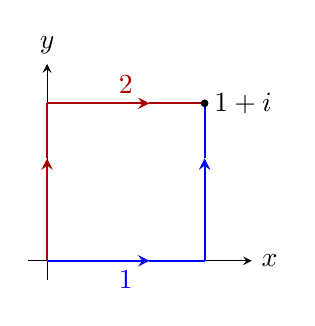
\begin{tikzpicture}[scale=2,>=stealth]
\draw[->](-.12,0)--(1.3,0)node[right]{$x$};
\draw[->](0,-.12)--(0,1.25)node[above]{$y$};
\draw[blue,thick,->](0,0)--(.65,0);
\draw[blue,thick](.65,0)--(1,0);
\draw[blue,thick,->](1,0)--(1,.65);
\draw[blue,thick](1,.65)--(1,1);
\draw[red!65!black,thick,->](0,0)--(0,.65);
\draw[red!65!black,thick](0,.65)--(0,1);
\draw[red!65!black,thick,->](0,1)--(.65,1);
\draw[red!65!black,thick](.65,1)--(1,1);
\fill(1,1)circle(.7pt)node[right]{$1+i$};
\node[blue,below]at(.5,0){1};
\node[red!65!black,above]at(.5,1){2};
\end{tikzpicture}
\end{center}

\Needspace{5\baselineskip}
\par\bigskip
\noindent\textbf{11.3.7}\quad Show that
\[
\oint_{C}\frac{dz}{z^{2}+z}=0,
\]
in which the contour $C$ is a \erratum{counterclockwise} circle defined by $|z|=R>1$.

\emph{Hint.}~Direct use of the Cauchy integral theorem is illegal. The
integral may be evaluated by expanding into partial fractions and then
treating the two terms individually. This yields $0$ for $R>1$ and $2\pi i$
for $\erratum{0<R<1}$.
\solution
Partial fractions give $1/[z(z+1)]=1/z-1/(z+1)$, since
$(z+1)-z=1$. For a counterclockwise circle, $\oint dz/(z-a)=2\pi i$ if
$a$ lies inside: the circle may be shrunk to $|z-a|=\rho$ without
crossing the singularity, and $z-a=\rho e^{i\theta}$ gives
$\int_0^{2\pi}i\,d\theta$. If $a$ lies outside, the integrand is
analytic on and inside the circle and Cauchy's theorem gives zero.
For $R>1$, both poles lie inside.
The two terms therefore contribute $2\pi i$ and $-2\pi i$,
giving $\boxed0$.
For $0<R<1$ only the origin lies inside; the term $1/(z+1)$ gives zero,
so the integral is $2\pi i$.
At $R=1$ the path hits $-1$, so the ordinary integral is undefined.
\erratum{The orientation matters for the hint's value $2\pi i$ at
$0<R<1$, which a clockwise circle changes to $-2\pi i$; the bound
$R>0$ excludes the degenerate circle $|z|=0$.}
The zero-integral theorem cannot be applied directly over the
singularities, which is why the decomposition is useful.

\Needspace{12\baselineskip}
\subsection*{11.4 Cauchy's Integral Formula}

Unless explicitly stated otherwise, closed contours occurring in these
exercises are to be understood as traversed in the mathematically positive
(counterclockwise) direction.

\Needspace{5\baselineskip}
\par\bigskip
\noindent\textbf{11.4.1}\quad Show that
\[
\frac{1}{2\pi i}\oint z^{m-n-1}\,dz,\quad m\text{ and }n\text{ integers}
\]
(with the contour encircling the origin once), is a representation of the
Kronecker $\delta_{mn}$.
\solution
On the circle $z=Re^{i\theta}$, $0\le\theta\le2\pi$, we have
$dz=iRe^{i\theta}d\theta$, so
$z^{m-n-1}dz=iR^{m-n}e^{i(m-n)\theta}d\theta$ and
\[
\frac1{2\pi i}\oint z^{m-n-1}\,dz
=\frac{R^{m-n}}{2\pi}\int_0^{2\pi}e^{i(m-n)\theta}\,d\theta.
\]
For $m=n$ this is $1$.
For the nonzero integer $k=m-n$, the integral is
$[e^{ik\theta}/(ik)]_0^{2\pi}=0$.
Thus the result is $\boxed{\delta_{mn}}$.
Contour deformation gives the same value for any contour avoiding
zero with positive winding number one.

\Needspace{5\baselineskip}
\par\bigskip
\noindent\textbf{11.4.2}\quad Evaluate
\[
\oint_{C}\frac{dz}{z^{2}-1},
\]
where $C$ is the circle $|z-1|=1$.
\solution
The poles at $1,-1$ have distances $0,2$ from the center $1$.
Only $1$ is inside the specified unit-radius circle.
Using
\[
\frac1{z^2-1}=\frac12\left(\frac1{z-1}-\frac1{z+1}\right),
\]
the first term contributes $\tfrac12\cdot2\pi i=\pi i$, since the circle
encloses $1$ (as in 11.3.7), and the second, analytic on and inside the
circle, integrates to zero by Cauchy's theorem.
Therefore $\boxed{\oint_C dz/(z^2-1)=\pi i}$.
\erratum{The Instructor's Manual's answer $0$ is incorrect for this contour:
the textbook (p.~491) prints the circle $|z-1|=1$, which encloses only
the pole at $z=1$.}

\Needspace{5\baselineskip}
\par\bigskip
\noindent\textbf{11.4.3}\quad Assuming that $f(z)$ is analytic on and within a
closed contour $C$ and that the point $z_{0}$ is within $C$, show that
\[
\oint_{C}\frac{f'(z)}{z-z_{0}}\,dz
=\oint_{C}\frac{f(z)}{(z-z_{0})^{2}}\,dz.
\]
\solution
Along the contour, the single-valued function $f(z)/(z-z_0)$ obeys
\[
d\left(\frac{f(z)}{z-z_0}\right)
=\left[\frac{f'(z)}{z-z_0}-\frac{f(z)}{(z-z_0)^2}\right]dz.
\]
Its closed integral is zero: the integral of the derivative of the
single-valued function $f(z)/(z-z_0)$, analytic on a neighborhood of
$C$, is the change of that function around the closed path. Moving one
term to the opposite side proves the stated equality. Both integrals also equal
$2\pi i f'(z_0)$ by Cauchy's formulas.

\Needspace{5\baselineskip}
\par\bigskip
\noindent\textbf{11.4.4}\quad You know that $f(z)$ is analytic on and within a
closed contour $C$, \erratum{with $z_0$ inside $C$ and $n$ a nonnegative integer.} You suspect that the $n$th derivative $f^{(n)}(z_{0})$ is
given by
\[
f^{(n)}(z_{0})=\frac{n!}{2\pi i}\oint_{C}\frac{f(z)}{(z-z_{0})^{n+1}}\,dz.
\]
Using mathematical induction (Section 1.4), prove that this expression is
correct.
\solution
The base case $n=0$ is Cauchy's integral formula. Assume the formula
holds for $n$ at every point inside $C$. The point $z_0$ has a positive
distance $\delta$ from $C$, so the disk $|\zeta-z_0|<\delta$, which
contains $z_0$ and does not meet $C$, lies inside $C$. Let
$0<|\Delta|<\delta/2$. Then $z_0+\Delta$ is inside $C$; subtracting the
formula at $z_0$ from the formula at $z_0+\Delta$ and dividing by
$\Delta$ gives
\[
\frac{f^{(n)}(z_0+\Delta)-f^{(n)}(z_0)}{\Delta}
=\frac{n!}{2\pi i}\oint_Cf(z)\,\frac{q(\Delta)-q(0)}{\Delta}\,dz,
\qquad q(s)=(z-z_0-s)^{-n-1}.
\]
Fix $z$ on $C$. By the chain rule,
\[
\begin{aligned}
q'(s)&=-(n+1)(z-z_0-s)^{-n-2}(-1)=(n+1)(z-z_0-s)^{-n-2},\\
q''(s)&=(n+1)(n+2)(z-z_0-s)^{-n-3}.
\end{aligned}
\]
On the segment from $0$ to $\Delta$, $|z-z_0-s|\ge\delta-|s|>\delta/2$,
so $|q''(s)|\le K$ with $K=(n+1)(n+2)(2/\delta)^{n+3}$. Integrating
$q''$ from $0$ to $s$ along the segment gives
$|q'(s)-q'(0)|\le K|s|\le K|\Delta|$ (Exercise 11.3.2), and integrating
$q'$ gives
\[
\left|\frac{q(\Delta)-q(0)}{\Delta}-q'(0)\right|
=\left|\frac1\Delta\int_0^\Delta[q'(s)-q'(0)]\,ds\right|
\le\frac{K|\Delta|\cdot|\Delta|}{|\Delta|}=K|\Delta|,
\]
a bound independent of $z$. Hence, by Exercise 11.3.2 with $L$ the
length of $C$,
\[
\left|\frac{f^{(n)}(z_0+\Delta)-f^{(n)}(z_0)}{\Delta}
-\frac{n!}{2\pi i}\oint_Cf(z)\,q'(0)\,dz\right|
\le\frac{n!}{2\pi}\Bigl(\max_C|f|\Bigr)L\,K|\Delta|\to0.
\]
The difference quotient therefore converges as $\Delta\to0$, and with
$q'(0)=(n+1)(z-z_0)^{-n-2}$ its limit is
\[
f^{(n+1)}(z_0)
=\frac{n!}{2\pi i}\oint_C
\frac{(n+1)f(z)}{(z-z_0)^{n+2}}\,dz
=\frac{(n+1)!}{2\pi i}\oint_C
\frac{f(z)}{(z-z_0)^{n+2}}\,dz.
\]
This is the induction step, proving the result for every $n\ge0$.

\Needspace{5\baselineskip}
\par\bigskip
\noindent\textbf{11.4.5}\quad
\begin{enumerate}
\item[(a)] A function $f(z)$ is analytic within a closed contour $C$ (and
  continuous on $C$). If $f(z)\neq0$ within $C$ and
  \erratum{$|f(z)|\ge m>0$} on $C$, show that
  \[
  \erratum{|f(z)|\ge m}
  \]
  for all points within $C$.

  \emph{Hint.}~Consider $w(z)=1/f(z)$.
\item[(b)] If $f(z)=0$ within the contour $C$, show that the foregoing result
  does not hold and that it is possible to have $|f(z)|=0$ at one or more
  points in the interior with $|f(z)|>0$ over the entire bounding contour.
  Cite a specific example of an analytic function that behaves this way.
\end{enumerate}
\solution
\erratum{As printed on p.~491, (a) reads: if $f(z)\ne0$ within $C$ and
$|f(z)|\le M$ on $C$, then $|f(z)|\le M$ for all points within $C$.
This maximum-modulus statement does not require $f\ne0$, so (b)'s
claim that it fails when $f$ has zeros is false. The hint $w=1/f$
points to the intended minimum-modulus statement given above. We prove
both.}
For the \textbf{original upper-bound version}, continuity gives a
maximum of $|f|$ on the closed bounded region (the inside of $C$
together with $C$). Suppose it exceeded $M$. Then it would occur at an
interior point $z_0$, with $f(z_0)\ne0$ because $|f(z_0)|>M\ge0$.
A constant $f$ is impossible, since its modulus would equal its
boundary value, at most $M$. For nonconstant $f$ some Taylor
coefficient at $z_0$ with $k\ge1$ is nonzero (identity theorem); with
the smallest such $k$,
$f(z_0+h)=f(z_0)+a_kh^k+O(h^{k+1})$, $a_k\ne0$.
Write $f(z_0)=|f(z_0)|e^{i\beta}$, $a_k=|a_k|e^{i\alpha}$, and take
$h=re^{i\theta}$ with $\theta=(\beta-\alpha)/k$. Then
$a_kh^k=|a_k|r^ke^{i\beta}$ has the phase of $f(z_0)$, so
$|f(z_0)+a_kh^k|=|f(z_0)|+|a_k|r^k$. The remainder is bounded by
$Kr^{k+1}$ for $0<r<r_0$, with some constants $K,r_0>0$, so
\[
|f(z_0+h)|\ge|f(z_0)|+|a_k|r^k-Kr^{k+1}>|f(z_0)|
\qquad\text{for }0<r<\min(r_0,|a_k|/K),
\]
contradicting maximality. Hence
$\boxed{|f|\le M}$ throughout, whether or not zeros occur.

For the \textbf{corrected lower bound in (a)}, assume $f$ has no zero on
the closed region and $|f|\ge m>0$ on $C$. Then $1/f$ is analytic
and obeys $|1/f|\le1/m$ on the boundary. The upper-bound result
gives $|1/f|\le1/m$ inside, hence $|f|\ge m$.
For \textbf{(b)}, $f(z)=z$ on the unit disk has boundary modulus
$1$ and $f(0)=0$. This disproves a positive interior \emph{lower}
bound without nonvanishing, while still satisfying the printed upper bound.

\Needspace{5\baselineskip}
\par\bigskip
\noindent\textbf{11.4.6}\quad Evaluate
\[
\oint_{C}\frac{e^{iz}}{z^{3}}\,dz,
\]
for the contour a square with sides of length $a>1$, centered at $z=0$.
\solution
Let $g=e^{iz}$, so $g''=i^2e^{iz}=-e^{iz}$. The square surrounds zero
once, so Cauchy's formula for the second derivative gives
\[
\oint_C\frac{e^{iz}}{z^3}\,dz
=\frac{2\pi i}{2!}g''(0)
=\pi i[-e^{iz}]_{z=0}=\boxed{-\pi i}.
\]
Any positive side length suffices; $a>1$ is stronger than needed.

\Needspace{5\baselineskip}
\par\bigskip
\noindent\textbf{11.4.7}\quad Evaluate
\[
\oint_{C}\frac{\sin^{2}z-z^{2}}{(z-a)^{3}}\,dz,
\]
where the contour encircles the point $z=a$.
\solution
Set $g(z)=\sin^2z-z^2$. Then, with $2\sin z\cos z=\sin2z$,
$g'=\sin2z-2z$ and $g''=2\cos2z-2$.
Cauchy's derivative formula gives
\[
\oint_C\frac{g(z)}{(z-a)^3}\,dz
=\frac{2\pi i}{2!}g''(a)
=\boxed{2\pi i(\cos2a-1)}.
\]
The formula still applies when a numerator zero lowers or removes
the apparent pole.

\Needspace{5\baselineskip}
\par\bigskip
\noindent\textbf{11.4.8}\quad Evaluate
\[
\oint_{C}\frac{dz}{z(2z+1)},
\]
for the contour the unit circle.
\solution
Decompose
\[
\frac1{z(2z+1)}=\frac1z-\frac2{2z+1}
=\frac1z-\frac1{z+1/2}.
\]
Both poles are inside the unit circle. Their contributions,
$2\pi i$ and $-2\pi i$, cancel, giving $\boxed0$.

\Needspace{5\baselineskip}
\par\bigskip
\noindent\textbf{11.4.9}\quad Evaluate
\[
\oint_{C}\frac{f(z)}{z(2z+1)^{2}}\,dz,
\]
for the contour the unit circle, \erratum{assuming $f$ is analytic on a neighborhood of the closed disk.}

\emph{Hint.}~Make a partial fraction expansion.
\solution
\erratum{Assume $f$ is analytic on and within the unit circle;
additional singularities would supply additional contributions.}
Write
$1/[z(2z+1)^2]=A/z+B/(2z+1)+D/(2z+1)^2$.
Clearing denominators yields
$1=A(2z+1)^2+Bz(2z+1)+Dz=(4A+2B)z^2+(4A+B+D)z+A$.
Constant, quadratic, and linear coefficients give, respectively,
$A=1$, $4A+2B=0$, $4A+B+D=0$; hence $B=-2$ and $D=-4-B=-2$.
Since $2/(2z+1)=1/(z+1/2)$ and $2/(2z+1)^2=\tfrac12/(z+1/2)^2$,
\[
\frac{f(z)}{z(2z+1)^2}
=\frac{f(z)}z-\frac{f(z)}{z+1/2}
-\frac{f(z)/2}{(z+1/2)^2}.
\]
Both points $0$ and $-1/2$ lie inside the unit circle. Cauchy's formula
$\oint f(z)\,dz/(z-z_0)=2\pi if(z_0)$ and its derivative form
$\oint f(z)\,dz/(z-z_0)^2=2\pi if'(z_0)$ now give
\[
2\pi if(0)-2\pi if(-1/2)-\tfrac12\cdot2\pi if'(-1/2)
=\boxed{2\pi i f(0)-2\pi i f(-1/2)-\pi i f'(-1/2)}.
\]

\Needspace{12\baselineskip}
\subsection*{11.5 Laurent Expansion}

\Needspace{5\baselineskip}
\par\bigskip
\noindent\textbf{11.5.1}\quad Develop the Taylor expansion of $\ln(1+z)$.
\par\nobreak\hfill\emph{ANS.}\enspace
$\displaystyle\sum_{n=1}^{\infty}(-1)^{n-1}\frac{z^{n}}{n}$.
\solution
Choose the logarithm analytic near $z=0$ with value zero there.
For $|z|<1$, the geometric series gives
$1/(1+z)=\sum_{n=0}^\infty(-1)^nz^n$.
It converges uniformly on every smaller closed disk, allowing
termwise integration from zero to $z$ along the segment. Since
$[\ln(1+z)]'=1/(1+z)$ and $\int_0^z\zeta^n\,d\zeta=z^{n+1}/(n+1)$,
and with the index shift $n+1\to n$ in the second form,
\[
\boxed{\ln(1+z)=\sum_{n=0}^\infty\frac{(-1)^nz^{n+1}}{n+1}
=\sum_{n=1}^\infty(-1)^{n-1}\frac{z^n}{n}}.
\]
Both sides vanish at zero, fixing the integration constant.
The nearest singularity is $z=-1$, so the Taylor radius is one.

\Needspace{5\baselineskip}
\par\bigskip
\noindent\textbf{11.5.2}\quad Derive the binomial expansion
\[
(1+z)^{m}=1+mz+\frac{m(m-1)}{1\cdot2}z^{2}+\cdots
=\sum_{n=0}^{\infty}\binom{m}{n}z^{n}
\]
for $m$, any real number. The expansion is convergent for $|z|<1$. Why?
\solution
Choose $(1+z)^m=\exp[m\operatorname{Log}(1+z)]$ with value $1$
at zero. For any real exponent $s$ the chain rule gives
$\frac{d}{dz}(1+z)^s=\exp[s\operatorname{Log}(1+z)]\,\frac{s}{1+z}
=s(1+z)^{s-1}$, so repeated differentiation gives
\[
\frac{d^n}{dz^n}(1+z)^m
=m(m-1)\cdots(m-n+1)(1+z)^{m-n}.
\]
Set $z=0$ and divide by $n!$ to obtain
\[
\boxed{(1+z)^m=\sum_{n=0}^\infty
\frac{m(m-1)\cdots(m-n+1)}{n!}z^n}.
\]
The empty product for $n=0$ is one. For a nonterminating series the
coefficients $c_n$ have $c_{n+1}/c_n=(m-n)/(n+1)$, so the absolute
successive-term ratio is $|z|\,|m-n|/(n+1)\to|z|$; by the ratio test
the series converges for $|z|<1$ and diverges for $|z|>1$.
The reason is the singularity at $z=-1$, where $1+z=0$: this branch is
analytic on the open disk $|z|<1$, which reaches up to $-1$, so by
Taylor's theorem the series converges to $(1+z)^m$ there, and no
larger disk about $0$ avoids $-1$.
For nonnegative integer $m$ the series terminates and is valid
everywhere; for other real $m$ the Taylor radius is one.

\Needspace{5\baselineskip}
\par\bigskip
\noindent\textbf{11.5.3}\quad A function $f(z)$ is analytic on and within the
unit circle. Also, $|f(z)| < 1$ for $|z| \le 1$ and $f(0)=0$. Show that
$|f(z)| < |z|$ for $\erratum{0<|z|\le1}$.

\emph{Hint.}~One approach is to show that $f(z)/z$ is analytic and then to
express $[f(z_{0})/z_{0}]^{n}$ by the Cauchy integral formula. Finally,
consider absolute magnitudes and take the $n$th root. This exercise is
sometimes called Schwarz's theorem.
\solution
\erratum{The strict inequality excludes $z=0$, where both sides
are zero. It holds for $0<|z|\le1$.}
The series $f(z)=a_1z+a_2z^2+\cdots$ shows that
$g(z)=f(z)/z$ extends analytically to zero by $g(0)=a_1$.
Compactness of the unit circle and the strict hypothesis give
$|g(\zeta)|=|f(\zeta)|\le M<1$ there.
For $|z_0|<1$, Cauchy's formula applied to the analytic function
$g^n$ gives the first relation below. On the circle
$|g(\zeta)^n|\le M^n$ and $|\zeta-z_0|\ge1-|z_0|$, so the bound of
Exercise 11.3.2, with length $2\pi$, gives the second:
\[
g(z_0)^n=\frac1{2\pi i}\oint_{|\zeta|=1}
\frac{g(\zeta)^n}{\zeta-z_0}\,d\zeta,\qquad
|g(z_0)|^n\le\frac1{2\pi}\cdot2\pi\cdot\frac{M^n}{1-|z_0|}
=\frac{M^n}{1-|z_0|}.
\]
Taking $n$th roots, $|g(z_0)|\le M(1-|z_0|)^{-1/n}$; letting
$n\to\infty$ gives $|g(z_0)|\le M$.
This also holds on the boundary. Thus
$|f(z)|\le M|z|<|z|$ for nonzero $z$, with equality $0=0$ at zero.

\Needspace{5\baselineskip}
\par\bigskip
\noindent\textbf{11.5.4}\quad If $f(z)$ is a real function of the complex
variable $z=x+iy$, that is, $f(x)=f^{*}(x)$ \erratum{for real $x$ near zero}, and the Laurent expansion about
the origin, $f(z)=\sum a_{n}z^{n}$ \erratum{on $0<|z|<R$}, has $a_{n}=0$ for $n < -N$, show that all
of the coefficients $a_{n}$ are real.

\emph{Hint.}~Show that $z^{N}f(z)$ is analytic (via Morera's theorem,
Section 11.4).
\solution
\erratum{Here \emph{real} means real-valued for real arguments
near the Laurent center, not throughout an open complex region.}
The finite principal part makes
\[
g(z)=z^Nf(z)=\sum_{j=0}^\infty a_{j-N}z^j
\]
analytic after its removable extension to zero.
For nonzero real $x$ near zero, $g(x)=x^Nf(x)$ is real, and
continuity gives a real value at zero. Each analytic derivative
at zero may be computed along the real line; derivatives of
this real-valued restriction are real. Hence
$a_{j-N}=g^{(j)}(0)/j!\in\mathbb R$ for every $j\ge0$.
The remaining coefficients vanish and are real as well.

\Needspace{5\baselineskip}
\par\bigskip
\noindent\textbf{11.5.5}\quad Prove that the Laurent expansion of a given
function about a given point is unique; that is, if
\[
f(z)=\sum_{n=-N}^{\infty}a_{n}(z-z_{0})^{n}
=\sum_{n=-N}^{\infty}b_{n}(z-z_{0})^{n},
\]
\erratum{with both series representing $f$ on a common annulus,} show that $a_{n}=b_{n}$ for all $n$.

\emph{Hint.}~Use the Cauchy integral formula.
\solution
Choose a circle $|\zeta-z_0|=r$ in the common convergence annulus.
Uniform convergence there permits termwise integration:
\[
\begin{aligned}
\frac1{2\pi i}\oint f(\zeta)(\zeta-z_0)^{-k-1}\,d\zeta
&=\sum_n a_n\frac1{2\pi i}\oint
(\zeta-z_0)^{n-k-1}\,d\zeta\\
&=\sum_n a_n\delta_{nk}=a_k.
\end{aligned}
\]
The circle integrals equal $\delta_{nk}$ by Exercise 11.4.1, applied in
the variable $\zeta-z_0$.
The second series gives $b_k$ for the identical integral.
Thus $\boxed{a_k=b_k}$ for every integer $k$.
The proof also works for an infinite principal part on a common annulus.
\erratum{The common annulus is needed because the proof integrates both
series over one circle on which both converge to $f$; about one point a
function can have different Laurent series on different annuli, e.g.,
the two expansions of $1/[z(z-1)]$ about $z=1$ in Exercise 11.6.10.}
For the displayed series, whose principal parts are finite, the
condition holds once both represent $f$ near $z_0$: each then does so on
a punctured disk $0<|z-z_0|<\varepsilon$, and the smaller of the two
disks is a common annulus.

\Needspace{5\baselineskip}
\par\bigskip
\noindent\textbf{11.5.6}\quad Obtain the Laurent expansion of $e^{z}/z^{2}$
about $z=0$.
\solution
Divide the everywhere-convergent exponential series by $z^2$:
\[
\boxed{\frac{e^z}{z^2}
=\sum_{n=0}^\infty\frac{z^{n-2}}{n!}
=\frac1{z^2}+\frac1z+\frac12+\frac z6+\frac{z^2}{24}+\cdots}.
\]
The annulus is $0<|z|<\infty$. The pole has order two and residue one.

\Needspace{5\baselineskip}
\par\bigskip
\noindent\textbf{11.5.7}\quad Obtain the Laurent expansion of
$ze^{z}/(z-1)$ about $z=1$.
\solution
Put $w=z-1$, so $z=1+w$ and $e^z=e\,e^w$. Then
\[
\frac{ze^z}{z-1}=\frac{(1+w)\,e\,e^w}{w}
=e\left(\frac1w+1\right)\sum_{n=0}^\infty\frac{w^n}{n!}.
\]
The $w^{-1}$ coefficient is $e$, from $n=0$ in the product with $1/w$.
For $m\ge0$ the $w^m$ coefficient comes from $n=m+1$ in the product
with $1/w$ and from $n=m$ in the product with $1$:
$e[1/(m+1)!+1/m!]=e[1+(m+1)]/(m+1)!=e(m+2)/(m+1)!$.
Consequently
\[
\boxed{\frac{ze^z}{z-1}
=\frac e{z-1}+e\sum_{m=0}^\infty
\frac{m+2}{(m+1)!}(z-1)^m},\qquad0<|z-1|<\infty.
\]
The first regular terms are $2e+\frac32e(z-1)+\frac23e(z-1)^2$.

\Needspace{5\baselineskip}
\par\bigskip
\noindent\textbf{11.5.8}\quad Obtain the Laurent expansion of
$(z-1)e^{1/z}$ about $z=0$.
\solution
Multiplication of the exponential series gives
\[
(z-1)e^{1/z}
=\sum_{n=0}^\infty\frac{z^{1-n}}{n!}
-\sum_{n=0}^\infty\frac{z^{-n}}{n!}.
\]
The leading term is $z$ ($n=0$ in the first sum), and the constants
($n=1$ in the first sum, $n=0$ in the second) cancel. For $k\ge1$ the
coefficient of $z^{-k}$ comes from $n=k+1$ in the first sum and $n=k$
in the second:
$1/(k+1)!-1/k!=[1-(k+1)]/(k+1)!=-k/(k+1)!$. Thus
\[
\boxed{(z-1)e^{1/z}
=z-\sum_{k=1}^\infty\frac{k}{(k+1)!}z^{-k}
=z-\frac1{2z}-\frac1{3z^2}-\frac1{8z^3}-\cdots}.
\]
It converges for $0<|z|<\infty$; its infinite principal part
makes zero an essential singularity.

\Needspace{12\baselineskip}
\subsection*{11.6 Singularities}

\Needspace{5\baselineskip}
\par\bigskip
\noindent\textbf{11.6.1}\quad As an example of an essential singularity
consider $e^{1/z}$ as $z$ approaches zero. For any complex number $z_{0}$,
$z_{0}\neq0$, show that
\[
e^{1/z}=z_{0}
\]
has an infinite number of solutions.
\solution
Write $z_0=\rho e^{i\alpha}$ with $\rho>0$, choosing one argument.
Since $e^w=e^{w'}$ exactly when $w-w'\in2\pi i\mathbb Z$, all solutions
of $e^w=z_0=e^{\ln\rho+i\alpha}$ are
$w=\ln\rho+i(\alpha+2\pi n)$, $n\in\mathbb Z$.
Therefore
\[
\boxed{z_n=\frac1{\ln\rho+i(\alpha+2\pi n)}}
\]
whenever the denominator is nonzero.
Substitution gives $e^{1/z_n}=\rho e^{i\alpha}=z_0$.
A zero denominator needs $\ln\rho=0$ and $\alpha+2\pi n=0$, so at most
one integer has one. All remaining denominators are distinct, since
their imaginary parts differ by multiples of $2\pi$, so their
reciprocals are distinct. Thus infinitely many distinct solutions
remain, with $|z_n|\le1/|\alpha+2\pi n|\to0$ as $|n|\to\infty$.
For $z_0=1$ with the choice $\alpha=0$, simply omit $n=0$.
\erratum{The Instructor's Manual argues from roots of truncated exponential polynomials. Passing to the limit does not by itself establish distinct roots of the original equation. The explicit logarithmic preimages above supply that missing argument.}

\Needspace{5\baselineskip}
\par\bigskip
\noindent\textbf{11.6.2}\quad Show that the function
\[
w(z)=(z^{2}-1)^{1/2}
\]
is single-valued if we make branch cuts on the real axis for $\erratum{x\ge1}$ and for $\erratum{x\le-1}$.
\solution
Remove both rays including their endpoints:
$D=\mathbb C\setminus((-\infty,-1]\cup[1,\infty))$.
For $z=x+iy$, $1-z^2=(1-x^2+y^2)-2ixy$ is nonpositive real only if
$xy=0$ and $1-x^2+y^2\le0$. The choice $x=0$ gives $1+y^2>0$;
otherwise $y=0$, $|x|\ge1$, exactly the removed rays.
The principal square root is analytic off the ray $(-\infty,0]$, so
$\sqrt{1-z^2}$ is analytic on $D$, and the explicit branch
\[
\boxed{w(z)=i\sqrt{1-z^2}}
\]
is single-valued and satisfies $w^2=z^2-1$.
Its negative is the other branch; one reference value selects its sign.
\erratum{The branch points $\pm1$ themselves are excluded from
the analytic domain, not merely the open rays.}
\erratum{The Instructor's Manual instead discusses a cut joining $-1$ to $1$. That is the different branch domain in Example 11.6.4, not the two outward rays specified here.}

\Needspace{5\baselineskip}
\par\bigskip
\noindent\textbf{11.6.3}\quad A function $f(z)$ can be represented by
\[
f(z)=\frac{f_{1}(z)}{f_{2}(z)},
\]
in which $f_{1}(z)$ and $f_{2}(z)$ are analytic. The denominator, $f_{2}(z)$,
vanishes at $z=z_{0}$, showing that $f(z)$ has a pole at $z=z_{0}$. However,
$f_{1}(z_{0})\neq0$, $f'_{2}(z_{0})\neq0$. Show that $a_{-1}$, the coefficient
of $(z-z_{0})^{-1}$ in a Laurent expansion of $f(z)$ at $z=z_{0}$, is given by
\[
a_{-1}=\frac{f_{1}(z_{0})}{f'_{2}(z_{0})}.
\]
\solution
With $h=z-z_0$, Taylor expansion gives
\[
f_1(z)=f_1(z_0)+O(h),\quad
f_2(z)=f'_2(z_0)h[1+O(h)].
\]
Each $O(h)$ here is a convergent power series in $h$ without constant
term. The last factor has an analytic reciprocal $1+O(h)$ near zero
because its constant term is one. Hence
\[
f(z)=\frac{f_1(z_0)+O(h)}{f'_2(z_0)h}[1+O(h)]
=\frac{f_1(z_0)}{f'_2(z_0)}h^{-1}+O(1).
\]
Therefore $\boxed{a_{-1}=f_1(z_0)/f'_2(z_0)}$.
The assumptions make this coefficient nonzero and the pole simple.

\Needspace{5\baselineskip}
\par\bigskip
\noindent\textbf{11.6.4}\quad Determine a unique branch for the function of
Exercise 11.6.2 that will cause the value it yields for $f(i)$ to be the same
as that found for $f(i)$ in Example 11.6.4. Although Exercise 11.6.2 and
Example 11.6.4 describe the same multivalued function, the specific values
assigned for various $z$ will not agree everywhere, due to the difference in
the location of the branch cuts. Identify the portions of the complex plane
where both these descriptions do and do not agree, and characterize the
differences.
\solution
Write $z-1=\rho_1e^{i\varphi_1}$ and $z+1=\rho_2e^{i\varphi_2}$. The
segment-cut branch $G$ of Example 11.6.4 is
$G(z)=(\rho_1\rho_2)^{1/2}e^{i(\varphi_1+\varphi_2)/2}$, positive on
the real axis $z>1$, where $\varphi_1=\varphi_2=0$.
At $z=i$, the arguments of $i-1$ and $i+1$ are $3\pi/4$ and
$\pi/4$ and their moduli are both $\sqrt2$. Its value is
\[
(\sqrt2)^{1/2}(\sqrt2)^{1/2}
e^{i(3\pi/4+\pi/4)/2}=\boxed{i\sqrt2}.
\]
The outward-cut branch with this value is
$F(z)=i\sqrt{1-z^2}$ from 11.6.2, since $F(i)=i\sqrt{1-i^2}=i\sqrt2$.
Since its domain is connected, the reference value fixes its sign;
the other branch, $-F$, has the value $-i\sqrt2$ there.

Where both are defined,
$F^2=G^2=z^2-1$ and neither vanishes; thus $F/G$ is continuous
and takes only $\pm1$, so it is constant on each connected piece of
the common domain. The two systems of cuts together cover the real
axis, so the common domain is the plane minus the real axis, whose
components are the upper and lower half-planes.
Equality at $i$ implies $F=G$ in the upper half-plane.
At $-i$, continuing $G$ from $z>1$ through the lower half-plane, the
arguments of $-i-1$ and $-i+1$ are $-3\pi/4$ and $-\pi/4$, so
$G(-i)=\sqrt2\,e^{-i\pi/2}=-i\sqrt2$, while
$F(-i)=i\sqrt{1-(-i)^2}=i\sqrt2$. Hence $F=-G$ in the lower half-plane.
On the real axis at most one of them is defined, since $G$ is cut along
$[-1,1]$ and $F$ along $|x|\ge1$. Each is continuous across the other's
cut, so by the half-plane relations its value there is the limit of the
other from above, written with argument $x+i0$, and minus the limit from
below, $x-i0$. For $|x|>1$, where $\varphi_1=\varphi_2$ is $0$ ($x>1$) or
$\pi$ ($x<-1$),
\[
G(x)=\operatorname{sgn}(x)\sqrt{x^2-1}=F(x+i0)=-F(x-i0),
\]
and for $|x|<1$, $F(x)=i\sqrt{1-x^2}=G(x+i0)=-G(x-i0)$.
These statements specify precisely their agreement and sign difference.
\erratum{The Instructor's Manual gives $f(i)=2i$. Each factor contributes modulus $2^{1/4}$, not $\sqrt2$, so their product has modulus $\sqrt2$. Also $(i\sqrt2)^2=-2=i^2-1$, whereas $(2i)^2=-4$.}

\Needspace{5\baselineskip}
\par\bigskip
\noindent\textbf{11.6.5}\quad Find all singularities of
\[
z^{-1/3}+\frac{z^{-1/4}}{(z-3)^{3}}+(z-2)^{1/2},
\]
and identify their types (e.g., second-order branch point, fifth-order pole,
\ldots). Include any singularities at the point at infinity.

\emph{Note.}~A branch point is of $n$th order if it requires $n$, but no
fewer, circuits around the point to restore the original value.
\solution
At zero, since $(z-3)^3=(-3)^3(1-z/3)^3$,
\[
\frac{z^{-1/4}}{(z-3)^3}
=-\frac1{27}z^{-1/4}(1-z/3)^{-3},
\]
where $(1-z/3)^{-3}$ and the third term $(z-2)^{1/2}$ are analytic
near zero. After $N$ circuits about zero the first two terms therefore
acquire multipliers $e^{-2\pi iN/3}$ and $e^{-2\pi iN/4}$, and the third
is unchanged, so the function changes by
\[
c_1z^{-1/3}+c_2z^{-1/4}(1-z/3)^{-3},\qquad
c_1=e^{-2\pi iN/3}-1,\quad c_2=-\tfrac1{27}\bigl(e^{-2\pi iN/4}-1\bigr).
\]
These changes cannot cancel. If $c_1\ne0$, the ratio of the second term
to the first, $(c_2/c_1)z^{1/12}(1-z/3)^{-3}$, tends to zero as $z\to0$
(because $-1/4-(-1/3)=1/12>0$), so the change is nonzero near zero; if
$c_1=0$, the change $c_2z^{-1/4}(1-z/3)^{-3}$ vanishes only if $c_2=0$.
Hence the function returns to its initial value iff both multipliers
equal $1$, i.e., iff $N$ is divisible by $3$ and $4$;
the least such positive integer is $12$. Zero is a branch point
of order $12$ in the question's convention.
At $3$, the chosen local numerator is analytic and nonzero and the
other two terms are analytic, giving a third-order pole. At $2$, only $(z-2)^{1/2}$ branches, with order $2$.
For infinity put $w=1/z$; with $(1/w-3)^3=(1-3w)^3/w^3$ and
$1/w-2=(1-2w)/w$,
\[
f(1/w)=w^{1/3}+\frac{w^{13/4}}{(1-3w)^3}
+w^{-1/2}(1-2w)^{1/2}.
\]
The analytic factors $(1-3w)^{-3}$ and $(1-2w)^{1/2}$ have nonzero
constant terms, so $N$ circuits about $w=0$ multiply the three terms by
$e^{2\pi iN/3}$, $e^{2\pi i(13N/4)}=e^{2\pi iN/4}$ (since
$e^{2\pi i\cdot3N}=1$) and $e^{-\pi iN}$. As at zero, the changes
cannot cancel: among the terms whose multiplier is not $1$, the one with
the smallest exponent of $w$ (the exponents are $-1/2<1/3<13/4$)
dominates the others as $w\to0$, so the change is nonzero near $w=0$.
So the function returns to its initial value iff all three multipliers
equal $1$, i.e., iff $N$ is divisible by $3$, $4$ and $2$; their least
common multiple is $12$.
Infinity is an order-$12$ branch point, not an isolated meromorphic pole.
There are no other finite singularities.

\Needspace{5\baselineskip}
\par\bigskip
\noindent\textbf{11.6.6}\quad The function $F(z)=\ln(z^{2}+1)$ is made
single-valued by straight-line branch cuts from $(x,y)=(0,-1)$ to
$(-\infty,-1)$ and from $(0,+1)$ to $(0,+\infty)$. See Fig.~11.17. If
$F(0)=-2\pi i$, find the value of $F(i-2)$.
\solution
Factor $z^2+1=(z-i)(z+i)$, so every branch has the form
$\ln|z-i|+\ln|z+i|+i[\arg(z-i)+\arg(z+i)]+2\pi ik$.
The upward cut from $i$ consists of the points with
$\arg(z-i)=\pi/2$; choosing $-3\pi/2<\arg(z-i)<\pi/2$ makes this
argument continuous off that cut. The leftward cut from $-i$ consists
of the points with $\arg(z+i)=\pi$; choosing $-\pi<\arg(z+i)<\pi$
makes this argument continuous off it.
At zero, $z-i=-i$ and $z+i=i$ have arguments $-\pi/2,\pi/2$ and both
moduli are one, so $F(0)=2\pi ik=-2\pi i$ requires $k=-1$.
The required branch is therefore
\[
F(z)=\ln|z-i|+\ln|z+i|
+i[\arg(z-i)+\arg(z+i)-2\pi].
\]
At $z=-2+i$, the factors are $-2$ and $-2+2i$.
Their arguments in these ranges are $-\pi$ and $3\pi/4$;
their moduli are $2$ and $2\sqrt2$. Thus
\[
F(i-2)=\ln2+\ln(2\sqrt2)+i\left(-\pi+\frac{3\pi}4-2\pi\right)
=\boxed{\ln(4\sqrt2)-9\pi i/4}.
\]
Exponentiation verifies the result:
$e^F=4\sqrt2\,e^{-9\pi i/4}=4\sqrt2\,e^{-i\pi/4}=4-4i=(-2+i)^2+1$.

\Needspace{5\baselineskip}
\par\bigskip
\noindent\textbf{11.6.7}\quad Show that negative numbers have logarithms in
the complex plane. In particular, find $\ln(-1)$.
\par\nobreak\hfill\emph{ANS.}\enspace $\erratum{\operatorname{Log}(-1)=i\pi\text{ (principal value)}}$.
\solution
For $r>0$, $-r=re^{i(\pi+2\pi n)}$, $n\in\mathbb Z$.
All logarithms are consequently
\[
\boxed{\ln(-r)=\ln r+i(2n+1)\pi}.
\]
In particular $\ln(-1)=i(2n+1)\pi$.
\erratum{The printed $i\pi$ is the principal value, or one chosen
branch value, rather than the complete multivalued answer.}

\Needspace{5\baselineskip}
\par\bigskip
\noindent\textbf{11.6.8}\quad For noninteger $m$, show that the binomial
expansion of Exercise 11.5.2 holds only for a suitably defined branch of the
function $(1+z)^{m}$. Show how the $z$-plane is cut. Explain why $|z| < 1$
may be taken as the circle of convergence for the expansion of this branch,
in light of the cut you have chosen.
\solution
Choose $(1+z)^m=\exp[m\operatorname{Log}(1+z)]$ with
$-\pi<\arg(1+z)<\pi$. The cut is $(-\infty,-1]$ and the
value at zero is $1$. This analytic branch has the Taylor
coefficients derived in 11.5.2, and the open unit disk avoids the cut.
For noninteger real $m$, a circuit about $-1$ increases $\arg(1+z)$ by
$2\pi$ and so multiplies the value by $e^{2\pi im}\ne1$. Thus $-1$ is a
genuine branch point, distance one from the Taylor center. The radius
is exactly one: if the series converged on a disk $|z|<\rho$ with
$\rho>1$, its sum $S$ would be analytic there and equal to the branch
on $|z|<1$, hence (by analytic continuation) on the disk minus the
cut. Continuing along a small circle about $-1$ inside the disk would
then return $S$ to its starting value, contradicting the factor
$e^{2\pi im}$.

\Needspace{5\baselineskip}
\par\bigskip
\noindent\textbf{11.6.9}\quad The Taylor expansion of Exercises 11.5.2 and
11.6.8 is not suitable for branches other than the one suitably defined
branch of the function $(1+z)^{m}$ for noninteger $m$. (Note that other
branches cannot have the same Taylor expansion since they must be
distinguishable.) Using the same branch cut of the earlier exercises for all
other branches, find the corresponding Taylor expansions, detailing the phase
assignments and Taylor coefficients.
\solution
For the same cut, let
\[
\operatorname{Log}_k(1+z)=\ln|1+z|
+i\arg(1+z)+2\pi ik,\quad k\in\mathbb Z,
\]
where the displayed argument lies in $(-\pi,\pi)$; the branch $k$
assigns $1+z$ the phase $\arg(1+z)+2\pi k$. Then
$(1+z)^m_k=\exp[m\operatorname{Log}_k(1+z)]
=e^{2\pi imk}\exp[m\operatorname{Log}_0(1+z)]=e^{2\pi imk}(1+z)^m_0$,
where $k=0$ is the branch of 11.6.8, so
\[
\boxed{(1+z)^m_k=e^{2\pi imk}
\sum_{n=0}^\infty\binom mn z^n,\qquad |z|<1}.
\]
Every coefficient is multiplied by the same phase; the constant
coefficient already distinguishes the branches.
For $m=p/q$ in lowest terms, $k$ modulo $q$ gives $q$ distinct
branches. For irrational $m$, all integer $k$ give distinct ones.

\Needspace{5\baselineskip}
\par\bigskip
\noindent\textbf{11.6.10}\quad
\begin{enumerate}
\item[(a)] Develop a Laurent expansion of $f(z)=[z(z-1)]^{-1}$ about the
  point $z=1$ valid for small values of $|z-1|$. Specify the exact range over
  which your expansion holds. This is an analytic continuation of the
  infinite series in Eq.~(11.49).
\item[(b)] Determine the Laurent expansion of $f(z)$ about $z=1$ but for
  $|z-1|$ large.
\end{enumerate}
\emph{Hint.}~Make a partial fraction decomposition of this function and use
the geometric series.
\solution
Put $w=z-1$, so $f=1/[w(1+w)]=1/w-1/(1+w)$, since $(1+w)-w=1$.
\textbf{(a)} For $|w|<1$, the geometric series
$1/(1+w)=\sum_{n=0}^\infty(-1)^nw^n$ gives
\[
\boxed{f=\frac1w-1+w-w^2+\cdots
=\sum_{n=-1}^\infty(-1)^{n+1}w^n,\qquad0<|w|<1}.
\]
The pole at $w=0$ excludes the center; the pole at $w=-1$
sets the outer radius.
\textbf{(b)} For $|w|>1$ write $w(1+w)=w^2(1+w^{-1})$ and expand
$(1+w^{-1})^{-1}=\sum_{n=0}^\infty(-1)^nw^{-n}$, a geometric series in
$w^{-1}$ with $|w^{-1}|<1$:
\[
\boxed{f=w^{-2}(1+w^{-1})^{-1}
=\sum_{n=0}^\infty(-1)^nw^{-n-2},\qquad |w|>1}.
\]
The annuli differ, so uniqueness of Laurent coefficients on a
fixed annulus is not contradicted.
\erratum{The Instructor's Manual writes the outer series as $\sum_{n=-2}^{\infty}(-1)^n(z-1)^{-n}$. Its lower index should be $2$; otherwise it begins with growing powers and cannot equal a function that decays as $(z-1)^{-2}$ at infinity.}

\Needspace{5\baselineskip}
\par\bigskip
\noindent\textbf{11.6.11}\quad
\begin{enumerate}
\item[(a)] Given $f_{1}(z)=\displaystyle\int_{0}^{\infty}e^{-zt}\,dt$ (with
  $t$ real), show that the domain in which $f_{1}(z)$ exists (and is
  analytic) is $\Re(z)>0$.
\item[(b)] Show that $f_{2}(z)=1/z$ equals $f_{1}(z)$ over $\Re(z)>0$ and is
  therefore an analytic continuation of $f_{1}(z)$ over the entire $z$-plane
  except for $z=0$.
\item[(c)] Expand $1/z$ about the point $z=-i$. You will have
  \[
  f_{3}(z)=\sum_{n=0}^{\infty}a_{n}(z+i)^{n}.
  \]
  What is the domain of this formula for $f_{3}(z)$?
\end{enumerate}
\par\nobreak\hfill\emph{ANS.}\enspace
$\dfrac{1}{z}=i\displaystyle\sum_{n=0}^{\infty}i^{-n}(z+i)^{n}$,\quad
$|z+i| < 1$.
\solution
\textbf{(a)} For $z\ne0$,
\[
\int_0^Te^{-zt}\,dt=(1-e^{-zT})/z.
\]
Here $|e^{-zT}|=e^{-T\Re z}$. If $\Re z>0$, the exponential tends to
zero as $T\to\infty$, so $f_1(z)=1/z$, which is analytic there.
If $\Re z<0$, $|e^{-zT}|$ grows without bound. If $\Re z=0$,
$z=iy\ne0$, then $e^{-iyT}$ has modulus one and keeps rotating, without
a limit. For $z=0$, the integral equals $T$.
Thus ordinary convergence occurs exactly on $\Re z>0$.
\textbf{(b)} By (a), $f_2=1/z$ equals $f_1$ on $\Re z>0$, and $1/z$ is
analytic on $\mathbb C\setminus\{0\}$. By the identity theorem it is
the only analytic function on this connected domain that agrees with
$f_1$ on $\Re z>0$; it is the analytic continuation of $f_1$.
\erratum{The continuation has no negative-integer singularities;
the Instructor's Manual's mention of those points is extraneous to this function.}
\textbf{(c)} Set $w=z+i$. Then $z=w-i=-i(1+iw)$ and $1/(-i)=i$; the
geometric series in $-iw$ converges for $|w|<1$, and
$(-i)^n=i^{-n}$ because $-i=1/i$, so
\[
\boxed{\frac1z=\frac i{1+iw}
=i\sum_{n=0}^\infty(-i)^nw^n
=i\sum_{n=0}^\infty i^{-n}(z+i)^n,\quad |z+i|<1}.
\]
The pole at zero is distance one from the center $-i$, fixing
the exact convergence radius.
\erratum{The Instructor's Manual expands about $+i$ in part (c), while the question requests $-i$. The expansion here uses $z+i$ and has constant coefficient $1/(-i)=i$.}

\Needspace{12\baselineskip}
\subsection*{11.7 Calculus of Residues}

\Needspace{5\baselineskip}
\par\bigskip
\noindent\textbf{11.7.1}\quad Determine the nature of the singularities of
each of the following functions and evaluate the residues ($a>0$).
\begin{enumerate}
\item[(a)] $\dfrac{1}{z^{2}+a^{2}}$.\qquad
(b) $\dfrac{1}{(z^{2}+a^{2})^{2}}$.\qquad
(c) $\dfrac{z^{2}}{(z^{2}+a^{2})^{2}}$.
\item[(d)] $\dfrac{\sin 1/z}{z^{2}+a^{2}}$.\qquad
(e) $\dfrac{ze^{iz}}{z^{2}+a^{2}}$.\qquad
(f) $\dfrac{ze^{iz}}{z^{2}-a^{2}}$.
\item[(g)] $\dfrac{e^{iz}}{z^{2}-a^{2}}$.\qquad
(h) $\dfrac{z^{-k}}{z+1}$,\quad $0 < k < 1$.
\end{enumerate}
\emph{Hint.}~For the point at infinity, use the transformation $w=1/z$ for
$|z|\to\erratum{\infty}$. For the residue, transform $f(z)\,dz$ into $g(w)\,dw$ and look at
the behavior of $g(w)$.
\solution
\erratum{Infinity corresponds to $w=1/z\to0$, hence to $|z|\to\infty$,
not to $|z|\to0$ as the printed hint says.} The nature of the
singularity at infinity is the nature of $f(1/w)$ at zero. For the
residue, $z=1/w$ gives $dz=-dw/w^2$, so $f(z)\,dz=g(w)\,dw$ with
$g(w)=-f(1/w)/w^2$, and, as the hint says, the residue at infinity is
that of $g$ at $w=0$:
\[
\operatorname{Res}_{\infty}f
=\operatorname{Res}_{w=0}\left[-\frac{f(1/w)}{w^2}\right].
\]
These are different transformations: the second includes the differential.

\textbf{(a)--(c)} Factor $z^2+a^2=(z-ia)(z+ia)$. For (a), both poles
are simple, and evaluating $(z\mp ia)f(z)=1/(z\pm ia)$ at $z=\pm ia$ gives
\[
\operatorname{Res}_{ia}\frac1{z^2+a^2}=\frac1{2ia},\qquad
\operatorname{Res}_{-ia}\frac1{z^2+a^2}=-\frac1{2ia}.
\]
For (b), the poles are double. The double-pole formula
$\operatorname{Res}_{z_0}f=\frac{d}{dz}[(z-z_0)^2f(z)]_{z=z_0}$, with
$(z-ia)^2f(z)=(z+ia)^{-2}$ and $(2ia)^3=8i^3a^3=-8ia^3$, gives
\[
\operatorname{Res}_{ia}\frac1{(z^2+a^2)^2}
=\left.\frac{d}{dz}(z+ia)^{-2}\right|_{ia}
=-\frac2{(2ia)^3}=\frac1{4ia^3}.
\]
Each of the functions (a)--(c) depends on $a$ only through $a^2$, so
replacing $a$ by $-a$ interchanges the poles $\pm ia$: the residue at
$-ia$ is the residue at $ia$ with $a\to-a$. For (b) it is
$-1/(4ia^3)$. In (c) the numerator $z^2$ equals $-a^2\ne0$ at $\pm ia$,
so the poles are again double, and the double-pole formula, now with
$(z-ia)^2f(z)=z^2/(z+ia)^2$, gives
\[
\left.\frac{d}{dz}\frac{z^2}{(z+ia)^2}\right|_{ia}
=\left.\frac{2z(z+ia)-2z^2}{(z+ia)^3}\right|_{ia}
=\frac{-2a^2}{-8ia^3}=\frac1{4ia}.
\]
The residue at $-ia$ is $-1/(4ia)$. At infinity the three functions
$f(1/w)$ become, after multiplying numerator and denominator by $w^2$
or $w^4$,
\[
\frac{w^2}{1+a^2w^2},\quad
\frac{w^4}{(1+a^2w^2)^2},\quad
\frac{w^2}{(1+a^2w^2)^2}.
\]
Thus infinity is removable, with a zero of order $2,4,2$, respectively.
The transformed differentials $g(w)=-f(1/w)/w^2$,
\[
-\frac1{1+a^2w^2},\quad
-\frac{w^2}{(1+a^2w^2)^2},\quad
-\frac1{(1+a^2w^2)^2},
\]
are analytic at $w=0$, so all three residues at infinity are zero.
Consistently, in each case the two finite residues add to zero.

\textbf{(d)} Zero is an essential singularity: if $f$ had at most a
pole there, so would $\sin(1/z)=(z^2+a^2)f(z)$, whose Laurent series
$\sum_{k\ge0}(-1)^kz^{-2k-1}/(2k+1)!$ has infinitely many negative
powers. The points $\pm ia$ are simple poles; as in (a), the residue
there is $\sin(1/z)/(z\pm ia)$ evaluated at $z=\pm ia$, where
$1/(\pm ia)=\mp i/a$ and $\sin(\mp i/a)=\mp i\sinh(1/a)$ (from
$\sin iy=i\sinh y$):
\[
\operatorname{Res}_{ia}f
=\frac{\sin(-i/a)}{2ia}
=-\frac{\sinh(1/a)}{2a},\qquad
\operatorname{Res}_{-ia}f
=\frac{\sin(i/a)}{-2ia}
=-\frac{\sinh(1/a)}{2a}.
\]
To obtain the residue at zero directly, multiply two series that
converge absolutely on $0<|z|<a$, the Laurent series of $\sin(1/z)$
above and the geometric series
$1/(z^2+a^2)=a^{-2}(1+z^2/a^2)^{-1}=\sum_{j\ge0}(-1)^jz^{2j}/a^{2j+2}$:
\[
\frac{\sin(1/z)}{z^2+a^2}
=\sum_{j,k\ge0}
\frac{(-1)^{j+k}z^{2j-2k-1}}{a^{2j+2}(2k+1)!}.
\]
A term has exponent $2j-2k-1=-1$ exactly when $j=k$, and then
$(-1)^{j+k}=1$. Consequently
\[
\boxed{\operatorname{Res}_{0}f
=\sum_{k=0}^{\infty}\frac1{a^{2k+2}(2k+1)!}
=\frac1a\sum_{k=0}^{\infty}\frac{(1/a)^{2k+1}}{(2k+1)!}
=\frac{\sinh(1/a)}a}.
\]
At infinity $f(1/w)=w^2\sin w/(1+a^2w^2)$ has a zero of order three,
since $\sin w=w+O(w^3)$, and $g(w)=-\sin w/(1+a^2w^2)$ is analytic at
$w=0$, so the residue at infinity is zero. Consistently, the three
finite residues add to zero.

\textbf{(e)--(g)} If $D$ has a simple zero $p$ and $N$ is analytic at
$p$, the residue of $N/D$ is $N(p)/D'(p)$, here with $D'(p)=2p$.
Applying this rule gives
\[
\begin{array}{c|c|c|c}
&\text{finite poles}&\text{residues in the same order}
&\operatorname{Res}_{\infty}f\\ \hline
(e)&ia,\,-ia&e^{-a}/2,\ e^{a}/2&-\cosh a\\
(f)&a,\,-a&e^{ia}/2,\ e^{-ia}/2&-\cos a\\
(g)&a,\,-a&e^{ia}/(2a),\ -e^{-ia}/(2a)&-i\sin a/a
\end{array}
\]
For example, the first two rows follow from
$p e^{ip}/(2p)=e^{ip}/2$ (for $p=\pm ia$ this is $e^{\mp a}/2$), and
the third from $e^{ip}/(2p)$ with $p=\pm a$.
All these finite poles are simple, since the numerators do not vanish
there. Each function has an essential singularity at infinity:
$f(1/w)$ is $e^{i/w}$ times a rational function of $w$ that is not
identically zero, so if $f(1/w)$ had at most a pole at $w=0$, so would
$e^{i/w}=\sum_{m\ge0}i^mw^{-m}/m!$, which has infinitely many negative
powers. Nevertheless its residue there is defined. Under $z=1/w$ a
small counterclockwise circle about $w=0$ becomes a large clockwise
circle $|z|=R$, so
$\operatorname{Res}_\infty f=-\frac1{2\pi i}\oint_{|z|=R}f\,dz$ with
the counterclockwise orientation. For $R>a$ the residue theorem gives
$\operatorname{Res}_{\infty}f=-\sum_{\text{finite }p}\operatorname{Res}_p f$.
The sums are $(e^{-a}+e^a)/2=\cosh a$, $(e^{ia}+e^{-ia})/2=\cos a$, and
$(e^{ia}-e^{-ia})/(2a)=i\sin a/a$, which yield the displayed answers.
\erratum{In (d), the Instructor's Manual gives positive residues at $\pm ia$; both must be $-\sinh(1/a)/(2a)$, as the displayed substitution shows. It reverses the paired exponents in (e), giving
$e^{\pm a}/2$ at $\pm ia$. Its (f) incorrectly uses poles $\pm ia$
and residues $-ie^{\mp a}/2$, although the denominator is $z^2-a^2$.
In (g) it reverses the exponential signs as well. Substitution into
$N(p)/D'(p)$ gives the table above, with each residue paired to its pole.}

\textbf{(h)} The nonintegral power produces branch points at zero and
infinity: continuation once around zero multiplies $z^{-k}$ by
$e^{-2\pi i k}\ne1$, while $f(1/w)=w^{-k}\cdot w/(1+w)=w^{k+1}/(1+w)$
is also multivalued at $w=0$. A rational $k=p/q$ in lowest terms gives
$q$ sheets; irrational $k$ gives infinitely many. On any local branch
at $-1$ the numerator is analytic and nonzero, so there is a simple
pole whose residue is the value of $z^{-k}$ at $-1$ on that branch,
$e^{-ik\arg(-1)}$ with $\arg(-1)=(2m+1)\pi$:
\[
\boxed{\operatorname{Res}_{-1}f=(-1)^{-k}
=e^{-ik(2m+1)\pi}}.
\]
For the branch $0<\arg z<2\pi$, $\arg(-1)=\pi$: take $m=0$, so the
residue is $e^{-ik\pi}$.
\erratum{The residue depends on the branch. Ordinary Laurent residues
at the branch points zero and infinity are not defined.}

\Needspace{5\baselineskip}
\par\bigskip
\noindent\textbf{11.7.2}\quad Evaluate the residues at $z=0$ and $z=-1$ of
$\pi\cot\pi z/z(z+1)$.
\solution
From $\cot x=\cos x/\sin x=x^{-1}(1-x^2/2+\cdots)(1-x^2/6+\cdots)^{-1}
=x^{-1}-x/3+O(x^3)$ with $x=\pi z$,
$\pi\cot\pi z=z^{-1}-(\pi^2/3)z+O(z^3)$. At zero, divide this by $z$
and expand $1/(1+z)$ in a geometric series:
\[
\frac{\pi\cot\pi z}{z(z+1)}
=\left(\frac1{z^2}-\frac{\pi^2}{3}+O(z^2)\right)
(1-z+z^2-\cdots)
=\frac1{z^2}-\frac1z+O(1).
\]
At $z=-1$, put $w=z+1$. The period one of $\cot\pi z$ gives
$\pi\cot\pi z=\pi\cot\pi w=w^{-1}+O(w)$, while $z(z+1)=(w-1)w$ and
$1/(w-1)=-(1+w+w^2+\cdots)$:
\[
\frac{\pi\cot\pi z}{z(z+1)}
=\frac{w^{-1}+O(w)}{w(w-1)}
=-\frac1{w^2}(1+w+w^2+\cdots)+O(1)
=-\frac1{w^2}-\frac1w+O(1).
\]
Thus both points are double poles and
\[
\boxed{\operatorname{Res}_{0}f=\operatorname{Res}_{-1}f=-1}.
\]

\Needspace{5\baselineskip}
\par\bigskip
\noindent\textbf{11.7.3}\quad The classical definition of the exponential
integral $\mathrm{Ei}(x)$ for $x>0$ is the Cauchy principal value integral
\[
\mathrm{Ei}(x)=\int_{-\infty}^{x}\frac{e^{t}}{t}\,dt,
\]
where the integration range is cut at $\erratum{t=0}$. Show that this definition yields
a convergent result for positive $x$.
\solution
\erratum{The printed problem says the range is cut at $x=0$; the
singular point of the integrand is $t=0$, while $x>0$ is the upper
limit.}
Fix $x>0$ and choose $0<\delta<x$. Split the negative side at $-x$
and change $t=-u$, $dt=-du$, in the interval $[-x,-\delta]$:
\[
\int_{-x}^{-\delta}\frac{e^t}{t}\,dt
=\int_{x}^{\delta}\frac{e^{-u}}{-u}\,(-du)
=-\int_\delta^x\frac{e^{-u}}u\,du.
\]
Inserting this after the split,
\[
\begin{aligned}
\int_{-\infty}^{-\delta}\frac{e^t}{t}\,dt+
\int_\delta^x\frac{e^t}{t}\,dt
&=\int_{-\infty}^{-x}\frac{e^t}{t}\,dt
-\int_\delta^x\frac{e^{-u}}u\,du
+\int_\delta^x\frac{e^u}u\,du\\
&=\int_{-\infty}^{-x}\frac{e^t}{t}\,dt
+\int_\delta^x\frac{e^u-e^{-u}}u\,du.
\end{aligned}
\]
The first integral converges absolutely, since $|e^t/t|\le e^t/x$ for
$t\le-x$ and $\int_{-\infty}^{-x}e^t\,dt=e^{-x}$. In the second,
$e^u-e^{-u}=2u+O(u^3)$, so the integrand has the finite limit $2$ at
zero; it extends continuously to $[0,x]$, and the integral over
$[\delta,x]$ tends to the integral over $[0,x]$ as $\delta\to0$.
Therefore
\[
\boxed{\mathrm{Ei}(x)=
\int_{-\infty}^{-x}\frac{e^t}{t}\,dt+
\int_0^x\frac{2\sinh u}{u}\,du}
\]
is finite. The cancellation uses equal distances $\delta$ on the two
sides of the pole, precisely the principal-value prescription.

\Needspace{5\baselineskip}
\par\bigskip
\noindent\textbf{11.7.4}\quad Writing a Cauchy principal value integral to
deal with the singularity at $x=1$, show that, if $0 < p < 1$,
\[
\int_{0}^{\infty}\frac{x^{-p}}{x-1}\,dx=\erratum{\pi\cot p\pi}.
\]
\solution
\erratum{For the printed denominator $x-1$, the answer is
$+\pi\cot(\pi p)$, not $-\pi\cot(\pi p)$. The Instructor's Manual derives its negative
answer for the different denominator $1-x$.}
Write the intended integral as
\[
I=\lim_{\delta\downarrow0}
\left(\int_0^{1-\delta}+\int_{1+\delta}^{\infty}\right)
\frac{x^{-p}}{x-1}\,dx.
\]
The endpoint estimates are $O(x^{-p})$ at zero and $O(x^{-p-1})$
at infinity, so $0<p<1$ makes both endpoints integrable. Only $x=1$
requires a principal value.

Use $F(z)=z^{-p}/(z-1)$ with $z^{-p}=|z|^{-p}e^{-ip\arg z}$,
$0<\arg z<2\pi$, and a keyhole contour about the positive real axis.
On the upper bank ($\arg z=0$) $z^{-p}=x^{-p}$; on the lower bank
($\arg z=2\pi$) it equals $q x^{-p}$, where $q=e^{-2\pi ip}$.
The upper bank, directed outward, gives $I$; the lower bank, directed
inward, gives $\int_\infty^0 qx^{-p}(x-1)^{-1}\,dx=-qI$; together they
give $(1-q)I$. Exclude the boundary pole at $1$ by semicircles of
radius $\delta$ into the domain. Near $z=1$, $z^{-p}\to1$ on the upper
bank and $z^{-p}\to q$ on the lower one, so there
$F(z)=1/(z-1)+O(1)$ and $F(z)=q/(z-1)+O(1)$, respectively. With
$z-1=\delta e^{i\theta}$, $\int dz/(z-1)=i\int d\theta$, while the
bounded remainder contributes $O(\delta)$. The upper semicircle runs
from $\theta=\pi$ to $\theta=0$ (clockwise) and contributes $-i\pi$; the
lower one runs from $\theta=0$ to $\theta=-\pi$ (also clockwise) and
contributes $-i\pi q$. On the origin circle
$|F|\le\epsilon^{-p}/(1-\epsilon)$ and on the outer circle
$|F|\le R^{-p}/(R-1)$; times the lengths $2\pi\epsilon$ and $2\pi R$,
these give $O(\epsilon^{1-p})$ and $O(R^{-p})$, so both vanish. No pole
remains inside the indented contour, hence
\[
(1-q)I-i\pi(1+q)=0.
\]
Finally, factoring out $e^{-\pi ip}$,
\[
1+q=e^{-\pi ip}(e^{\pi ip}+e^{-\pi ip})=2e^{-\pi ip}\cos\pi p,\qquad
1-q=2ie^{-\pi ip}\sin\pi p,
\]
and therefore
\[
\boxed{\PVint_0^\infty\frac{x^{-p}}{x-1}\,dx
=i\pi\frac{1+q}{1-q}=i\pi\frac{\cos\pi p}{i\sin\pi p}=\pi\cot\pi p}.
\]
An independent check of the sign: $x=1/u$ turns the part beyond
$1+\delta$ into $\int_0^{1/(1+\delta)}u^{p-1}(1-u)^{-1}\,du$. Its piece
between $1-\delta$ and $1/(1+\delta)$ has length $\delta^2/(1+\delta)$
and integrand at most $(1-\delta)^{p-1}(1+\delta)/\delta$, so it
vanishes as $\delta\to0$. Hence
\[
\PVint_0^\infty\frac{x^{-p}}{x-1}\,dx
=\int_0^1\frac{x^{p-1}-x^{-p}}{1-x}\,dx,
\]
an ordinary integral, since the numerator vanishes at $x=1$. For
$0<p<\frac12$ we have $p-1<-p$, so the integrand is positive on
$(0,1)$; the integral is positive, like $\pi\cot\pi p$, whereas
$-\pi\cot\pi p<0$.

\Needspace{5\baselineskip}
\par\bigskip
\noindent\textbf{11.7.5}\quad Explain why Eq.~(11.88) is not directly
applicable to the product expansion of $\sin z$. Show how the expansion,
Eq.~(11.89), can be obtained by expanding instead $\sin z/z$.
\solution
The product formula quoted in the text contains the factors
$f(0)$ and $\exp[zf'(0)/f(0)]$. Since $\sin0=0$, direct substitution
would both annihilate the product and divide by zero. Instead let
\[
g(z)=\begin{cases}\sin z/z,&z\ne0,\\1,&z=0.\end{cases}
\]
The Taylor expansion $g(z)=1-z^2/3!+z^4/5!-\cdots$ gives
$g(0)=1$ and $g'(0)=0$. Its zeros are the nonzero points $\pm n\pi$,
each simple. To justify the product for this specific function,
differentiate $\ln g=\ln\sin z-\ln z$ and use the cotangent pole
expansion (11.81), together with
$\frac{d}{dz}\operatorname{Log}[1-z^2/(n^2\pi^2)]
=[-2z/(n^2\pi^2)]/[1-z^2/(n^2\pi^2)]$: on $|z|<\pi$,
\[
\frac{g'(z)}{g(z)}=\cot z-\frac1z
=\sum_{n=1}^{\infty}\frac{2z}{z^2-n^2\pi^2}
=\sum_{n=1}^{\infty}\frac{d}{dz}
\operatorname{Log}\!\left(1-\frac{z^2}{n^2\pi^2}\right).
\]
The removable value at zero is understood. On every smaller closed disk
the summands are bounded by a constant times $n^{-2}$, so the series
converges uniformly and may be integrated from zero to $z$.
Choose the analytic logarithms that vanish at zero; since $g$ has no zero
in this disk and $g(0)=1$, integration gives
\[
\operatorname{Log}g(z)=\sum_{n=1}^{\infty}
\operatorname{Log}\!\left(1-\frac{z^2}{n^2\pi^2}\right).
\]
Exponentiating yields the paired product. Equivalently, the canonical
factors of (11.88) for $g$, with $g(0)=1$, $g'(0)=0$ (so the
exponential prefactor is $1$) and the opposite zeros $\pm n\pi$, give
\[
g(z)=\prod_{n=1}^{\infty}
\left(1-\frac{z}{n\pi}\right)e^{z/(n\pi)}
\left(1+\frac{z}{n\pi}\right)e^{-z/(n\pi)}.
\]
Pairing the positive and negative zeros cancels the exponentials and
multiplies the two linear factors:
\[
\boxed{\sin z=z\prod_{n=1}^{\infty}
\left(1-\frac{z^2}{n^2\pi^2}\right)}.
\]
The paired product converges uniformly on compact sets because
$\sum_{n\ge1}|z|^2/(n^2\pi^2)$ does. It defines an entire function,
so its equality to $g$ on $|z|<\pi$ extends to the whole plane by the
identity theorem. Multiplication by $z$ proves the displayed formula,
including its simple zero and derivative one at zero.
\erratum{The statement preceding (11.88) needs additional restrictions:
zeros and the two values $f(0),f'(0)$ do not determine an arbitrary entire
function. For example, $e^{z^2}$ has no zeros, $f(0)=1$, and $f'(0)=0$,
while that formula would give $1$. The logarithmic-derivative argument
above establishes the sine product without this unjustified generalization.}

\Needspace{5\baselineskip}
\par\bigskip
\noindent\textbf{11.7.6}\quad Starting from the observations
\begin{enumerate}
\item[1.] $f(z)=a_n z^n$ has $n$ zeros \erratum{counted with multiplicity, where $a_n\ne0$ and $n\ge1$,} and
\item[2.] for sufficiently large $|R|$,
  $\left|\sum_{m=0}^{n-1}a_{m}R^{m}\right| < |a_{n}R^{n}|$,
\end{enumerate}
use Rouch\'e's theorem to prove the fundamental theorem of algebra (namely
that every polynomial of degree $n$ has $n$ roots).
\solution
\erratum{The monomial $a_nz^n$ has the single zero $z=0$, so it has
$n$ zeros only when they are counted with multiplicity; and it has
degree $n\ge1$ only if $a_n\ne0$.}
Let
\[
P(z)=a_nz^n+\sum_{m=0}^{n-1}a_mz^m,\qquad a_n\ne0,
\quad S=\sum_{m=0}^{n-1}|a_m|.
\]
Choose $R>\max(1,S/|a_n|)$. At every point of $|z|=R$, the triangle
inequality, $R^m\le R^{n-1}$ for $m\le n-1$ (as $R>1$), and
$S<|a_n|R$ give
\[
\left|\sum_{m=0}^{n-1}a_mz^m\right|
\le\sum_{m=0}^{n-1}|a_m|R^m
\le SR^{n-1}<|a_n|R^n=|a_nz^n|.
\]
Rouch\'e's theorem (if $|g|<|f|$ on a closed contour, then $f$ and
$f+g$ have the same number of zeros inside it), with $f=a_nz^n$ and
$g=P-a_nz^n$, says that $P$ and $a_nz^n$ have the same number
of zeros inside this circle. The monomial has its sole zero at zero,
of multiplicity $n$, so $P$ has exactly $n$ zeros there. The same
inequality holds for every larger radius. Any additional finite zero
would lie within some such larger circle and increase the count,
which is impossible. Thus $P$ has exactly $n$ complex roots with
multiplicity.

\Needspace{5\baselineskip}
\par\bigskip
\noindent\textbf{11.7.7}\quad Using Rouch\'e's theorem, show that all the
zeros of $F(z)=z^{6}-4z^{3}+10$ lie between the circles $|z|=1$ and $|z|=2$.
\solution
Rouch\'e's theorem: if $|g|<|f|$ on a closed contour, then $f$ and
$f+g$ have the same number of zeros inside it.
On $|z|=1$ compare $F$ with the constant $f=10$, taking
$g=z^6-4z^3$:
\[
|z^6-4z^3|\le|z|^6+4|z|^3=1+4=5<10.
\]
The constant has no zeros, so Rouch\'e's theorem gives no zeros in
$|z|<1$; on the circle itself $|F|\ge10-5>0$, so there is no zero
there either. On $|z|=2$, compare with $f=z^6$, taking $g=-4z^3+10$:
\[
|-4z^3+10|\le4(2^3)+10=42<2^6=64.
\]
Since $z^6$ has six zeros (at the origin, with multiplicity), there
are six zeros of $F$ in $|z|<2$, counted with multiplicity, and none
on its boundary, where $|F|\ge64-42>0$. A degree-six polynomial has
exactly six zeros, so all lie in $1<|z|<2$.
As an independent check, setting $w=z^3$ yields
$w^2-4w+10=0$, hence $w=(4\pm\sqrt{16-40})/2=2\pm i\sqrt6$. Both values
have modulus $\sqrt{4+6}=\sqrt{10}$, so every root satisfies
$|z|=|w|^{1/3}=10^{1/6}\approx1.468$, strictly between one and two.
\erratum{The Instructor's Manual claims $|z^6+10|>|-4z^3|$ for all points inside $|z|=2$. It fails when $z^3=i\sqrt{10}$: the left side is zero and the right side is positive. The comparisons above apply on the two boundary circles, as required by Rouch\'e's theorem.}

\Needspace{5\baselineskip}
\par\bigskip
\noindent\textbf{11.7.8}\quad Derive the pole expansions of $\sec z$ and
$\csc z$ given in Eqs.~(11.82) and (11.83).
\solution
A simple pole of $1/h$ at a simple zero $a$ of $h$ has residue
$1/h'(a)$. Thus, with $a_n=(n+\tfrac12)\pi$, $(\cos z)'=-\sin z$,
$\sin(\pm a_n)=\pm(-1)^n$, and $(\sin z)'=\cos z$, $\cos n\pi=(-1)^n$,
\[
\operatorname{Res}_{a_n}\sec z=(-1)^{n+1},\quad
\operatorname{Res}_{-a_n}\sec z=(-1)^n,\qquad
\operatorname{Res}_{n\pi}\csc z=(-1)^n.
\]
To justify a pole expansion, integrate $F(\zeta)/(\zeta-z)$ on
expanding rectangles, with $z$ fixed inside. For $\sec\zeta$, use
vertical sides $\Re\zeta=\pm N\pi$ and horizontal sides
$\Im\zeta=\pm N\pi$. On a vertical side
$\cos(\pm N\pi+iy)=\cos N\pi\cosh y\mp i\sin N\pi\sinh y=(-1)^N\cosh y$,
so $|\sec\zeta|=\operatorname{sech}y$, and $|\zeta-z|\ge N\pi-|z|$;
its integral is at most
$(N\pi-|z|)^{-1}\int_{\mathbb R}\operatorname{sech}y\,dy=\pi/(N\pi-|z|)$,
which is $O(N^{-1})$.
On a horizontal side
$|\cos(x\pm iN\pi)|^2=\cos^2x+\sinh^2N\pi\ge\sinh^2N\pi$, so its
integral is at most $2N\pi/[(N\pi-|z|)\sinh N\pi]$ and
tends to zero exponentially. For $\csc\zeta$, choose vertical sides
$\Re\zeta=\pm(N+\tfrac12)\pi$ and the same horizontal heights.
There $\sin(\pm(N+\tfrac12)\pi+iy)=\pm(-1)^N\cosh y$, so
$|\csc\zeta|=\operatorname{sech}y$, while
$|\sin(x\pm iN\pi)|^2=\sin^2x+\sinh^2N\pi$;
the estimates are the same.

Inside the rectangle, $F(\zeta)/(\zeta-z)$ has residue $F(z)$ at
$\zeta=z$ and residue $\operatorname{Res}_aF/(a-z)$ at each pole $a$
of $F$. Since the contour integral tends to zero, the residue theorem
gives, in the limit,
\[
0=F(z)+\sum_a\frac{\operatorname{Res}_a F}{a-z},
\qquad
F(z)=\sum_a\frac{\operatorname{Res}_a F}{z-a}.
\]
The $N$th rectangle contains the poles $\pm a_n$, $n<N$, for $\sec$, and
$0,\pm\pi,\dots,\pm N\pi$ for $\csc$, so the sums are limits of
symmetric partial sums. For $\sec z$ pair the poles $a_n$ and $-a_n$:
\[
\frac{(-1)^{n+1}}{z-a_n}+\frac{(-1)^n}{z+a_n}
=\frac{2(-1)^na_n}{a_n^2-z^2}.
\]
For $\csc z$ separate the pole at zero and pair $\pm n\pi$:
\[
\frac{(-1)^n}{z-n\pi}+\frac{(-1)^n}{z+n\pi}
=\frac{2(-1)^nz}{z^2-n^2\pi^2}.
\]
Consequently, using $2a_n=(2n+1)\pi$ and $a_n^2=(n+\tfrac12)^2\pi^2$,
off their poles,
\[
\boxed{\sec z=\pi\sum_{n=0}^{\infty}
\frac{(-1)^n(2n+1)}{(n+\tfrac12)^2\pi^2-z^2}},\qquad
\boxed{\csc z=\frac1z+2z\sum_{n=1}^{\infty}
\frac{(-1)^n}{z^2-n^2\pi^2}}.
\]
The second paired series is absolutely locally uniformly convergent.
In the first, the leading term is the convergent alternating series
$2(-1)^n/a_n$, and subtracting that leading term leaves
$2(-1)^nz^2/[a_n(a_n^2-z^2)]$, a locally uniform $O(n^{-3})$ series. This specifies the pairing and convergence
needed for the pole expansion.

\Needspace{5\baselineskip}
\par\bigskip
\noindent\textbf{11.7.9}\quad Given that $f(z)=(z^{2}-3z+2)/z$, apply a
partial fraction decomposition to $f'/f$ and show directly that
$\oint_{C}f'(z)/f(z)\,dz=2\pi i(N_{f}-P_{f})$, where $N_{f}$ and $P_{f}$ are,
respectively, the numbers of zeros and poles encircled by $C$ (including
their multiplicities), \erratum{for a simple positively oriented contour avoiding $0,1,2$.}
\solution
Here $f(z)=z-3+2/z=(z-1)(z-2)/z$ and $f'(z)=1-2/z^2=(z^2-2)/z^2$, so
\[
\frac{f'}f=\frac{z^2-2}{z(z-1)(z-2)}
=\frac Az+\frac B{z-1}+\frac C{z-2}.
\]
Multiplying by each linear factor and setting $z$ equal to its root
gives $A=(-2)/[(-1)(-2)]=-1$, $B=(-1)/[1\cdot(-1)]=1$, and
$C=2/(2\cdot1)=1$:
\[
\frac{f'}f=\frac1{z-1}+\frac1{z-2}-\frac1z.
\]
For a positively oriented simple closed contour through none of
$0,1,2$, $\oint_C dz/(z-c)$ equals $2\pi i$ if $c$ is inside (Cauchy's
integral formula) and zero if $c$ is outside (Cauchy's theorem). So
each of the first two fractions integrates to $2\pi i$
if its pole is inside and to zero otherwise. The last contributes
$-2\pi i$ if zero is inside. The zeros of $f$ are $1,2$ and its only
pole is $0$, all simple. Hence
\[
\boxed{\oint_C\frac{f'}f\,dz
=2\pi i\bigl(\mathbf1_{\{1\text{ inside}\}}
+\mathbf1_{\{2\text{ inside}\}}-\mathbf1_{\{0\text{ inside}\}}\bigr)
=2\pi i(N_f-P_f)}.
\]
\erratum{For a general closed curve the same formula uses winding-number
weighted counts; the unweighted interpretation assumes a simple
positively oriented contour avoiding all zeros and poles.}

\Needspace{5\baselineskip}
\par\bigskip
\noindent\textbf{11.7.10}\quad \erratum{For a shrinking semicircle about a simple pole,
the limiting contribution is one-half the full-circle integral, with
compatible orientation.} Show, by a specific example, that
\[
\int_{\text{Semicircle}}f(z)\,dz
=\frac{1}{2}\oint_{\text{Circle}}f(z)\,dz
\]
does not necessarily hold if the integral encircles a pole of higher order.

\emph{Hint.}~Try $f(z)=z^{-2}$.
\solution
\erratum{Even for a simple pole the equality holds only in the limit:
if $f=a_{-1}/(z-z_0)+g$ with $g$ analytic, the semicircle
$z-z_0=Re^{i\theta}$, $0\le\theta\le\pi$, gives $i\pi a_{-1}+O(R)$,
which tends to $\frac12(2\pi ia_{-1})$, half the full-circle integral,
as $R\to0$.}
Take $f(z)=z^{-2}$ and the upper semicircle $z=Re^{i\theta}$,
$0\le\theta\le\pi$. Since $dz=iRe^{i\theta}\,d\theta$, the integrand
is $iRe^{i\theta}/(R^2e^{2i\theta})\,d\theta=(i/R)e^{-i\theta}\,d\theta$,
and with the antiderivative $e^{-i\theta}/(-i)$ and $e^{-i\pi}=-1$,
\[
\int_{\text{upper arc}}\frac{dz}{z^2}
=\frac iR\int_0^\pi e^{-i\theta}\,d\theta
=-\frac1R[e^{-i\theta}]_0^\pi=-\frac1R(-1-1)=\frac2R.
\]
On the full circle the same computation gives
$-R^{-1}[e^{-i\theta}]_0^{2\pi}=0$, since $e^{-2\pi i}=1$; equivalently,
the residue of $z^{-2}$ at zero is zero.
Thus $2/R\ne\frac12(0)$ for every $R>0$; the semicircle integral
even diverges as the radius shrinks. The cancellation on the other
half of the circle is essential for a pole of order two.

\Needspace{5\baselineskip}
\par\bigskip
\noindent\textbf{11.7.11}\quad A function $f(z)$ is analytic along the real
axis except for a third-order pole at $z=x_{0}$. The Laurent expansion about
$z=x_{0}$ has the form
\[
f(z)=\frac{a_{-3}}{(z-x_{0})^{3}}+\frac{a_{-1}}{z-x_{0}}+g(z),
\]
with $g(z)$ analytic at $z=x_{0}$. \erratum{Assume the integrals converge separately at both infinite endpoints.} Show that the Cauchy principal value
technique is applicable, in the sense that
\begin{enumerate}
\item[(a)] $\displaystyle\lim_{\delta\to0}
  \left\{\int_{-\infty}^{x_{0}-\delta}f(x)\,dx
  +\int_{x_{0}+\delta}^{\infty}f(x)\,dx\right\}$ is finite.
\item[(b)] $\displaystyle\erratum{\lim_{\delta\downarrow0}}\int_{C_{x_{0}}}f(z)\,dz=\pm i\pi a_{-1}$,
\end{enumerate}
where $C_{x_{0}}$ denotes a semicircle \erratum{of radius $\delta$} about $z=x_{0}$.
\solution
\erratum{The hypothesis controls the singularity at $x_0$, but does not
ensure convergence at infinity. Part (a) needs convergent tails, or a
separately specified principal value there. For instance
$f(z)=(z-x_0)^{-3}+1$ satisfies the local hypothesis and has divergent
tails. Also, the equality in (b) is a limit as the semicircle shrinks.}
Assume the tails in (a) converge, and choose $h>0$ within the Laurent
expansion's disk. Put $t=x-x_0$. The singular terms are odd, so for
$j=1,3$ and every $0<\delta<h$,
\[
\int_{-h}^{-\delta}t^{-j}\,dt+\int_\delta^h t^{-j}\,dt=0;
\]
indeed, the substitution $t=-u$, $dt=-du$, gives
$\int_{-h}^{-\delta}t^{-j}\,dt=\int_h^\delta(-u)^{-j}(-du)
=-\int_\delta^hu^{-j}\,du$ for odd $j$.
Meanwhile continuity of $g$ gives
\[
\lim_{\delta\downarrow0}
\left(\int_{x_0-h}^{x_0-\delta}g(x)\,dx+
\int_{x_0+\delta}^{x_0+h}g(x)\,dx\right)
=\int_{x_0-h}^{x_0+h}g(x)\,dx.
\]
Adding the two nonsingular convergent tails proves local principal-value
existence and thus the qualified statement (a).

On a semicircle set $z-x_0=\delta e^{i\theta}$, so
$dz=i\delta e^{i\theta}\,d\theta$ and $dz/(z-x_0)^3
=i\delta^{-2}e^{-2i\theta}\,d\theta$. Then
\[
\int \frac{a_{-3}\,dz}{(z-x_0)^3}
=ia_{-3}\delta^{-2}\int_{\theta_1}^{\theta_2}e^{-2i\theta}\,d\theta
=ia_{-3}\delta^{-2}\left[\frac{e^{-2i\theta}}{-2i}\right]_{\theta_1}^{\theta_2}=0,
\qquad \theta_2-\theta_1=\pm\pi,
\]
because the endpoint values of $e^{-2i\theta}$ are equal
($e^{\mp2\pi i}=1$). The simple pole contributes
$a_{-1}\int i\,d\theta=ia_{-1}(\theta_2-\theta_1)=\pm i\pi a_{-1}$.
Finally, by the ML inequality, the analytic part is bounded by the
length $\pi\delta$ times $\max_{|z-x_0|=\delta}|g(z)|$, which tends to
zero. Therefore
\[
\boxed{\lim_{\delta\downarrow0}\int_{C_{x_0}}f(z)\,dz
=\pm i\pi a_{-1}},
\]
with plus for counterclockwise traversal and minus for clockwise traversal.

\Needspace{5\baselineskip}
\par\bigskip
\noindent\textbf{11.7.12}\quad The unit step function is defined as (compare
Exercise \erratum{1.11.9})
\[
u(s-a)=\begin{cases}
0, & s<a\\
1, & s>a.
\end{cases}
\]
Show that $u(s)$ has the integral representations
\begin{enumerate}
\item[(a)] $u(s)=\displaystyle\lim_{\epsilon\to0^{+}}\frac{1}{2\pi i}
  \erratum{\displaystyle\int_{-\infty}^{\infty}}\frac{e^{ixs}}{x-i\epsilon}\,dx$.
\item[(b)] $u(s)=\dfrac{1}{2}+\dfrac{1}{2\pi i}\displaystyle
  \PVint_{-\infty}^{\infty}\frac{e^{ixs}}{x}\,dx$.
\end{enumerate}
\emph{Note.}~The parameter $s$ is real \erratum{and nonzero; the symmetric convention at $s=0$ is discussed below.}
\solution
\erratum{The published erratum removes the principal-value symbol in
(a): for fixed $\epsilon>0$ the pole is off the real axis. For $s\ne0$
the ordinary oscillatory improper integral exists. At $s=0$ its two
tails do not converge separately; a symmetric limit assigns $u(0)=1/2$,
while the problem's definition leaves $u(0)$ unspecified.}
\erratum{The printed cross-reference, Exercise 1.15.13, does not exist
in this edition, whose Chapter 1 ends with Section 1.11; the step
function is introduced in Exercise 1.11.9 as the limit of
$u_n(x)=\frac12(1+\tanh nx)$.}
For $s>0$, close the contour in the upper half-plane. The exponential
has modulus $|e^{izs}|=e^{-s\,\Im z}\le1$ there, and
$1/(z-i\epsilon)=O(R^{-1})$ on the arc $|z|=R$, so Jordan's estimate
makes the large semicircle contribution tend to zero. The sole pole is
$z=i\epsilon$ and has residue $e^{i(i\epsilon)s}=e^{-\epsilon s}$. Thus
\[
\frac1{2\pi i}\int_{\mathbb R}\frac{e^{ixs}}{x-i\epsilon}\,dx
=\frac{2\pi i\,e^{-\epsilon s}}{2\pi i}
=e^{-\epsilon s}\longrightarrow1.
\]
For $s<0$, close below, where $|e^{izs}|=e^{|s|\Im z}\le1$ and Jordan's
estimate applies again. There are no poles below the real axis, so the
clockwise contour gives zero. These are exactly the two prescribed step
values.

For (b), evaluate
$J(s)=\PVint_{\mathbb R}e^{ixs}/x\,dx$ directly. The integrand
$e^{izs}/z$ has a simple pole at zero with residue $1$. For $s>0$
close above and indent the origin into the upper half-plane.
The small clockwise arc has limit $-i\pi\cdot1$; the indented domain
contains no pole. Hence $J(s)-i\pi=0$. For $s<0$, close below;
the lower indentation is counterclockwise and contributes $+i\pi$,
so $J(s)+i\pi=0$. Consequently, with
$J(s)/(2\pi i)=\frac12\operatorname{sgn}s$,
\[
J(s)=i\pi\,\operatorname{sgn}s,\qquad
\boxed{\frac12+\frac{J(s)}{2\pi i}
=\frac{1+\operatorname{sgn}s}{2}=u(s)\quad(s\ne0)}.
\]
For completeness the connection between the prescriptions is visible in
\[
\frac1{x-i\epsilon}
=\frac{x}{x^2+\epsilon^2}
+i\frac{\epsilon}{x^2+\epsilon^2}.
\]
The second term has integral $i\pi$ in the limit: put
$x=\epsilon t$, then use dominated convergence with $(1+t^2)^{-1}$.
The first tends to the principal-value term (pair the two sides near
zero and use oscillatory convergence in the tails). At $s=0$,
the symmetric integral of the first term is zero and that of the second
is $i\pi$, giving the optional value $1/2$ in both representations.

\Needspace{12\baselineskip}
\subsection*{11.8 Evaluation of Definite Integrals}

\Needspace{5\baselineskip}
\par\bigskip
\noindent\textbf{11.8.1}\quad Generalizing Example 11.8.1, \erratum{for real $a,b$,} show that
\[
\int_{0}^{2\pi}\frac{d\theta}{a\pm b\cos\theta}
=\int_{0}^{2\pi}\frac{d\theta}{a\pm b\sin\theta}
=\frac{2\pi}{(a^{2}-b^{2})^{1/2}},\quad\text{for }a>|b|.
\]
What happens if $|b|>|a|$?
\solution
Take $a,b$ real (the condition $a>|b|$ and the final question
presuppose this) with $a>|b|$, and first consider $a+b\cos\theta$.
If $b=0$, the integral is $2\pi/a$. Otherwise set
$z=e^{i\theta}$, $d\theta=dz/(iz)$, $\cos\theta=(z+z^{-1})/2$, and
$D=\sqrt{a^2-b^2}>0$. Then $a+b\cos\theta=(bz^2+2az+b)/(2z)$, so
\[
I=\oint_{|z|=1}\frac{2z}{bz^2+2az+b}\,\frac{dz}{iz}
=\frac2i\oint_{|z|=1}\frac{dz}{bz^2+2az+b}.
\]
By the quadratic formula the roots of the denominator are $(-a\pm D)/b$;
multiplying numerator and denominator by $a+D$ and using
$D^2-a^2=-b^2$,
\[
r_+=\frac{-a+D}{b}=-\frac b{a+D},\qquad
r_-=\frac{-a-D}{b},\qquad r_+r_-=\frac bb=1.
\]
Since $|r_+|=|b|/(a+D)<1$ and $|r_-|=1/|r_+|>1$, only $r_+$ is inside.
The residue of the rational integrand there is the reciprocal of the
derivative $2bz+2a$ of its denominator at $r_+$:
\[
\frac1{2br_++2a}=\frac1{2(-a+D)+2a}=\frac1{2D}.
\]
The residue theorem gives
\[
\boxed{I=\frac2i(2\pi i)\frac1{2D}
=\frac{2\pi}{\sqrt{a^2-b^2}}}.
\]
The derivation holds for either sign of $b$, so changing $b$ to $-b$
leaves the result unchanged. Since $\sin\theta=\cos(\theta-\pi/2)$,
the substitution $\varphi=\theta-\pi/2$ turns the sine integrals into
cosine integrals over $[-\pi/2,3\pi/2]$, and a full-period integral of
a $2\pi$-periodic function does not depend on where the period starts,
proving the other two formulas.

If $|b|>|a|$, the denominator vanishes at the angles $\theta_0$ with
$\cos\theta_0=-a/b$ (or the corresponding sine values), which exist
because $|a/b|<1$. Its derivative $-b\sin\theta_0$ there is nonzero
because $|\cos\theta_0|<1$. Locally the reciprocal
therefore has the form $c/(\theta-\theta_0)+O(1)$, $c\ne0$, which is
not integrable.
\erratum{The ordinary improper integrals then do not exist. An analytic
continuation of the displayed square root is not their value; any
principal-value prescription must be specified separately.}
If principal values are taken at both zeros, the roots
$r_\pm=(-a\pm i\sqrt{b^2-a^2})/b$ lie on $|z|=1$, and each contributes
$\pi i$ times its residue (half the usual $2\pi i$) to the contour
integral, namely $\pi i/(2br_\pm+2a)=\pi i/(\pm2i\sqrt{b^2-a^2})$.
These cancel, so the principal value is zero.

\Needspace{5\baselineskip}
\par\bigskip
\noindent\textbf{11.8.2}\quad Show that
\[
\int_{0}^{\pi}\frac{d\theta}{(a+\cos\theta)^{2}}
=\frac{\pi a}{(a^{2}-1)^{3/2}},\quad a>1.
\]
\solution
For $a>1$, the substitution $\theta\mapsto2\pi-\theta$, which leaves
$\cos\theta$ unchanged, maps $[\pi,2\pi]$ onto $[0,\pi]$; so the
integral over $[0,\pi]$ is half the full-period integral of
Exercise 11.8.1 with $b=1$:
\[
J(a)=\int_0^\pi\frac{d\theta}{a+\cos\theta}
=\frac12\cdot\frac{2\pi}{\sqrt{a^2-1}}=\frac{\pi}{\sqrt{a^2-1}}.
\]
On any closed interval of parameters lying in $(1,\infty)$, the
denominator is bounded away from zero, and the $a$-derivative
$-(a+\cos\theta)^{-2}$ of the integrand is continuous. We may therefore
differentiate under the finite integral, and by the chain rule
$\frac{d}{da}(a^2-1)^{-1/2}=-\frac12(a^2-1)^{-3/2}\cdot2a$:
\[
J'(a)=-\int_0^\pi\frac{d\theta}{(a+\cos\theta)^2}
=-\pi a(a^2-1)^{-3/2}.
\]
Multiplying by $-1$ proves
\[
\boxed{\int_0^\pi\frac{d\theta}{(a+\cos\theta)^2}
=\frac{\pi a}{(a^2-1)^{3/2}}}.
\]

\Needspace{5\baselineskip}
\par\bigskip
\noindent\textbf{11.8.3}\quad Show that
\[
\int_{0}^{2\pi}\frac{d\theta}{1-2t\cos\theta+t^{2}}
=\frac{2\pi}{1-t^{2}},\quad\text{for }|t| < 1.
\]
What happens if $|t|>1$? What happens if $|t|=1$?
\solution
For $t\ne0$ write, with $z=e^{i\theta}$ and $z+1/z=2\cos\theta$,
\[
(1-tz)(1-t/z)=1-t(z+1/z)+t^2=1-2t\cos\theta+t^2.
\]
With $d\theta=dz/(iz)$ and $z(1-t/z)=z-t$,
\[
I(t)=\oint_{|z|=1}\frac{dz}{iz(1-tz)(1-t/z)}
=\frac1i\oint_{|z|=1}
\frac{dz}{(1-tz)(z-t)}.
\]
The two poles are $z=t$ and $z=1/t$. If $|t|<1$, only $t$ is inside
and its residue is $1/(1-t\cdot t)=1/(1-t^2)$, so
$I=(1/i)(2\pi i)/(1-t^2)$. If $|t|>1$, only $1/t$ is inside; writing
$1-tz=-t(z-1/t)$, its residue is
$1/[-t(1/t-t)]=1/(t^2-1)$. Therefore
\[
\boxed{I(t)=
\begin{cases}2\pi/(1-t^2),&|t|<1,\\
2\pi/(t^2-1),&|t|>1.
\end{cases}}
\]
The case $t=0$ directly gives $2\pi$, consistent with the first branch.
These calculations also hold for complex $t$ off the unit circle.

For real $t$ with $|t|=1$, the denominator is
$2(1-\cos\theta)=4\sin^2(\theta/2)$ at $t=1$ and
$2(1+\cos\theta)=4\cos^2(\theta/2)$ at $t=-1$. Each has a quadratic
zero (at $\theta=0,2\pi$ and at $\theta=\pi$, respectively), near which
the positive integrand behaves like $(\theta-\theta_0)^{-2}$, and
the integral diverges to $+\infty$.
\erratum{If complex $t$ is admitted, the other points $|t|=1$ put
simple poles on the integration path instead. Those ordinary improper
integrals are also undefined; they need not diverge to positive infinity.}

\Needspace{5\baselineskip}
\par\bigskip
\noindent\textbf{11.8.4}\quad Evaluate
\[
\int_{0}^{2\pi}\frac{\cos3\theta\,d\theta}{5-4\cos\theta}.
\]
\par\nobreak\hfill\emph{ANS.}\enspace $\pi/12$.
\solution
Because $\sin3\theta/(5-4\cos\theta)$ changes sign under
$\theta\mapsto2\pi-\theta$, which maps $[0,2\pi]$ onto itself, its
integral equals its own negative and vanishes. We may thus
replace $\cos3\theta$ by $e^{3i\theta}=\cos3\theta+i\sin3\theta$
without changing the desired integral. With $z=e^{i\theta}$,
$e^{3i\theta}=z^3$, $d\theta=dz/(iz)$, and
$5-4\cos\theta=5-2(z+z^{-1})=(-2z^2+5z-2)/z$, so
\[
I=\oint_{|z|=1}\frac{z^3\cdot z}{-2z^2+5z-2}\,\frac{dz}{iz}
=\frac1i\oint_{|z|=1}
\frac{z^3\,dz}{-2z^2+5z-2}.
\]
The denominator is $-(2z-1)(z-2)=-2(z-\tfrac12)(z-2)$, so only $z=1/2$
lies inside. Its residue is
\[
\left.\frac{z^3}{-2(z-2)}\right|_{z=1/2}
=\frac{1/8}{(-2)(-3/2)}=\frac{1/8}{3}=\frac1{24}.
\]
It follows that
\[
\boxed{I=\frac1i(2\pi i)\frac1{24}=\frac{\pi}{12}}.
\]

\Needspace{5\baselineskip}
\par\bigskip
\noindent\textbf{11.8.5}\quad With the calculus of residues, show that
\[
\int_{0}^{\pi}\cos^{2n}\theta\,d\theta
=\pi\frac{(2n)!}{2^{2n}(n!)^{2}}
=\pi\frac{(2n-1)!!}{(2n)!!},\quad n=0,1,2,\ldots.
\]
The double factorial notation is defined in Eq.~(1.76).

\emph{Hint.}~$\cos\theta=\frac{1}{2}(e^{i\theta}+e^{-i\theta})
=\frac{1}{2}(z+z^{-1})$,\quad $|z|=1$.
\solution
The even power has period $\pi$, since
$\cos^{2n}(\theta+\pi)=(-\cos\theta)^{2n}=\cos^{2n}\theta$, so twice
the required integral is its integral over $[0,2\pi]$. Set
$z=e^{i\theta}$, so that $\cos^{2n}\theta=2^{-2n}(z+z^{-1})^{2n}$,
$d\theta=dz/(iz)$, and $(z+z^{-1})^{2n}=z^{-2n}(z^2+1)^{2n}$:
\[
2I_n=\frac1{i\,2^{2n}}\oint_{|z|=1}
\frac{(z+z^{-1})^{2n}}z\,dz
=\frac1{i\,2^{2n}}\oint_{|z|=1}
\frac{(z^2+1)^{2n}}{z^{2n+1}}\,dz.
\]
Expand the numerator,
$(z^2+1)^{2n}=\sum_{j=0}^{2n}\binom{2n}{j}z^{2j}$.
The $z^{-1}$ term occurs when $2j-(2n+1)=-1$, or $j=n$,
and has coefficient $\binom{2n}{n}$, which is therefore the residue.
Hence, by the residue theorem,
\[
2I_n=\frac{2\pi i}{i\,2^{2n}}\binom{2n}{n}
=\frac{2\pi}{2^{2n}}\binom{2n}{n},\qquad
\boxed{I_n=\pi\frac{(2n)!}{2^{2n}(n!)^2}}.
\]
Finally $(2n)!!=2\cdot4\cdots(2n)=2^n n!$ and
$(2n-1)!!=(2n)!/(2n)!!=(2n)!/(2^n n!)$, so
$(2n-1)!!/(2n)!!=(2n)!/(2^{2n}(n!)^2)$, the factorial ratio above. For $n=0$ the empty-product convention
$(-1)!!=0!!=1$ gives $I_0=\pi$ as required.

\Needspace{5\baselineskip}
\par\bigskip
\noindent\textbf{11.8.6}\quad Verify that simplification of the expression in
Eq.~(11.112) yields the result given in Eq.~(11.113).
\solution
In the cited example,
$I=\int_0^\infty\ln x/(1+x^3)\,dx$. Put
$q=e^{2\pi i/3}=-\tfrac12+i\tfrac{\sqrt3}{2}$.
Equation (11.112), as printed in the textbook, reads
\[
(1-q)I-\frac{2\pi i}{3}q\,\frac{2\pi}{3\sqrt3}
=(2\pi i)\frac{\pi i}{9}q^{-1}.
\]
Move the second term to the right and use $i^2=-1$:
\[
(1-q)I=-\frac{2\pi^2}{9}q^{-1}
+\frac{4\pi^2i}{9\sqrt3}q.
\]
Since $q^{-1}=-\tfrac12-i\tfrac{\sqrt3}{2}$ and
$iq=-\tfrac{\sqrt3}{2}-\tfrac i2$, the two terms are
$-\frac{2\pi^2}{9}q^{-1}$ and
$\frac{4\pi^2}{9\sqrt3}(iq)$, that is,
\[
\frac{\pi^2}{9}+\frac{i\pi^2\sqrt3}{9},
\qquad
-\frac{2\pi^2}{9}-\frac{2i\pi^2}{9\sqrt3}.
\]
Since $\sqrt3/9-2/(9\sqrt3)=(3-2)/(9\sqrt3)$, their sum is
$-\pi^2/9+i\pi^2/(9\sqrt3)
=-(2\pi^2/27)(\tfrac32-i\tfrac{\sqrt3}{2})$, where
$\sqrt3/27=1/(9\sqrt3)$ was used.
But $1-q=\tfrac32-i\tfrac{\sqrt3}{2}\ne0$. Canceling this factor gives
\[
\boxed{I=-\frac{2\pi^2}{27}},
\]
which is Eq.~(11.113).

\Needspace{5\baselineskip}
\par\bigskip
\noindent\textbf{11.8.7}\quad Complete the details of Example 11.8.8 by
verifying that there is no contribution to the contour integral from either
the small or the large circles of the contour, and that Eq.~(11.115)
simplifies to the result given as (11.116).
\solution
Use $F(z)=z^p/(1+z^2)$ with $0<\arg z<2\pi$, and let the keyhole
run outward along the upper bank and inward along the lower bank.
\erratum{This orientation reverses the incorrectly drawn lower arrows
in the textbook's Fig.~11.26, as specified in the published errata.}
On the small circle $|z|=\epsilon<1$, $|z^p|=\epsilon^p$ and
$|1+z^2|\ge1-\epsilon^2$; with the length $2\pi\epsilon$,
\[
\left|\int_{\text{small}}F(z)\,dz\right|
\le\frac{2\pi\epsilon^{p+1}}{1-\epsilon^2}\longrightarrow0.
\]
On the large circle $|z|=R>1$, $|z^p|=R^p$ and $|1+z^2|\ge R^2-1$:
\[
\left|\int_{\text{large}}F(z)\,dz\right|
\le\frac{2\pi R^{p+1}}{R^2-1}
=O(R^{p-1})\longrightarrow0.
\]
Thus the two arc contributions vanish for $-1<p<1$, in particular
for the stated $0<p<1$.

The upper bank ($\arg z=0$, $z^p=x^p$) contributes $I$; on the lower
bank $z^p=x^pe^{2\pi ip}$ and the direction is inward, so it
contributes $-e^{2\pi ip}I$. The residues at $i$ and $-i$ are
$z^p/(z+i)$ at $i$ and $z^p/(z-i)$ at $-i$; with arguments
$\pi/2$ and $3\pi/2$ on this branch they are
\[
\frac{e^{ip\pi/2}}{2i},\qquad
-\frac{e^{3ip\pi/2}}{2i}.
\]
Multiplying their sum by $2\pi i$ and factoring out $e^{ip\pi}$,
\[
(1-e^{2\pi ip})I
=\pi(e^{ip\pi/2}-e^{3ip\pi/2})
=\pi e^{ip\pi}(e^{-ip\pi/2}-e^{ip\pi/2})
=-2\pi i e^{ip\pi}\sin(p\pi/2).
\]
Also $1-e^{2\pi ip}=e^{ip\pi}(e^{-ip\pi}-e^{ip\pi})
=-2ie^{ip\pi}\sin p\pi$.
For $0<p<1$ these factors are nonzero. Dividing,
$I=\pi\sin(p\pi/2)/\sin p\pi$, and
$\sin p\pi=2\sin(p\pi/2)\cos(p\pi/2)$ gives
\[
\boxed{I=\int_0^\infty\frac{x^p}{1+x^2}\,dx
=\frac{\pi}{2\cos(p\pi/2)}}.
\]
The same result extends throughout $-1<p<1$, with $p=0$ obtained
by continuity or directly from $\int_0^\infty dx/(1+x^2)=\pi/2$.

\Needspace{5\baselineskip}
\par\bigskip
\noindent\textbf{11.8.8}\quad Evaluate
\[
\int_{-\infty}^{\infty}\frac{\cos bx-\cos ax}{x^{2}}\,dx,\quad a>b>0.
\]
\par\nobreak\hfill\emph{ANS.}\enspace $\pi(a-b)$.
\solution
Consider $F(z)=(e^{ibz}-e^{iaz})/z^2$. From
$e^{icz}=1+icz-c^2z^2/2+O(z^3)$,
$e^{ibz}-e^{iaz}=i(b-a)z+(a^2-b^2)z^2/2+O(z^3)$, so
\[
F(z)=\frac{e^{ibz}-e^{iaz}}{z^2}
=\frac{i(b-a)}z+\frac{a^2-b^2}{2}+O(z).
\]
Close the real line above and indent the origin by a small clockwise
upper semicircle of radius $\epsilon$. On the large arc $|z|=R$,
$|e^{iaz}|,|e^{ibz}|\le1$ (since $\Im z\ge0$), so $|F|\le2/R^2$ and,
with the length $\pi R$, the arc integral is bounded by $2\pi/R$ and
vanishes. On the small arc, $z=\epsilon e^{i\theta}$ with $\theta$ from
$\pi$ to $0$, the term $i(b-a)/z$ contributes
$i(b-a)\int_\pi^0i\,d\theta=-i\pi[i(b-a)]=\pi(b-a)$, while the bounded
remainder contributes $O(\epsilon)$. There are no poles inside
the indented contour, hence
\[
\PVint_{\mathbb R}F(x)\,dx+\pi(b-a)=0,\qquad
\PVint_{\mathbb R}F(x)\,dx=\pi(a-b).
\]
Taking real parts removes the simple pole: the real integrand
$(\cos bx-\cos ax)/x^2$ tends to $(a^2-b^2)/2$ at zero and is
absolutely integrable at infinity. Thus it needs no principal value,
and
\[
\boxed{\int_{\mathbb R}\frac{\cos bx-\cos ax}{x^2}\,dx
=\pi(a-b)}.
\]
The same proof allows $b=0$, since the large-arc estimate still holds.

\Needspace{5\baselineskip}
\par\bigskip
\noindent\textbf{11.8.9}\quad Prove that
\[
\int_{-\infty}^{\infty}\frac{\sin^{2}x}{x^{2}}\,dx=\erratum{\pi}.
\]
\emph{Hint.}~$\sin^{2}x=\frac{1}{2}(1-\cos2x)$.
\solution
Use $\sin^2x=(1-\cos2x)/2$ and the case $b=0$, $a=2$ of
Exercise 11.8.8, which gives $\int_{\mathbb R}(1-\cos2x)x^{-2}\,dx
=\pi(2-0)=2\pi$:
\[
\int_{\mathbb R}\frac{\sin^2x}{x^2}\,dx
=\frac12\int_{\mathbb R}\frac{1-\cos2x}{x^2}\,dx
=\frac12(2\pi)=\boxed{\pi}.
\]
The origin is removable with limiting value one, and the tails are
bounded by $x^{-2}$, so this is an ordinary absolutely convergent
integral.
\erratum{The textbook prints the limits $-\infty$ to $\infty$
but gives $\pi/2$, and the errata list of the Instructor's Manual
(p.~3) also states $\pi/2$; that is the half-line value
$\int_0^\infty(\sin x/x)^2\,dx$. The Instructor's Manual's worked
solution (p.~138) correctly gives $\pi$ for the full line and $\pi/2$
for the half-line. Evenness and the contour calculation above prove
that the full-line value is $\pi$.}

\Needspace{5\baselineskip}
\par\bigskip
\noindent\textbf{11.8.10}\quad Show that
\[
\int_{0}^{\infty}\frac{x\sin x}{x^{2}+1}\,dx=\frac{\pi}{2e}.
\]
\solution
Integrate $F(z)=ze^{iz}/(z^2+1)$ over an upper semicircle.
Its rational factor is bounded by $R/(R^2-1)=O(R^{-1})$ on the large
arc, and $|e^{iz}|=e^{-\Im z}$ decays in the upper half-plane, so
Jordan's estimate ($\int_{\text{arc}}|e^{iz}|\,|dz|<\pi$) bounds that
arc by $\pi R/(R^2-1)$, which vanishes. The only enclosed pole is $i$:
\[
\operatorname{Res}_{i}F
=\left.\frac{ze^{iz}}{z+i}\right|_{z=i}=\frac{ie^{-1}}{2i}
=\frac{e^{-1}}2.
\]
Therefore
\[
\int_{\mathbb R}\frac{xe^{ix}}{x^2+1}\,dx=2\pi i\,\frac{e^{-1}}2
=\frac{\pi i}{e}.
\]
The real part $x\cos x/(x^2+1)$ is odd and integrates to zero over
$[-R,R]$. The imaginary part $x\sin x/(x^2+1)$ is even, so its
full-line integral, $\pi/e$, is twice the required one:
\[
\boxed{\int_0^\infty\frac{x\sin x}{x^2+1}\,dx=\frac{\pi}{2e}}.
\]
The tails converge by Dirichlet's test (the amplitude
$x/(x^2+1)$ decreases to zero for $x>1$), although they are not
absolutely convergent.

\Needspace{5\baselineskip}
\par\bigskip
\noindent\textbf{11.8.11}\quad A quantum mechanical calculation of a
transition probability leads to the function
$f(t,\omega)=2(1-\cos\omega t)/\omega^{2}$. Show that
\[
\int_{-\infty}^{\infty}f(t,\omega)\,d\omega=\erratum{2\pi|t|},\qquad\erratum{t\in\mathbb R}.
\]
\solution
\erratum{For a general real time parameter the answer is $2\pi|t|$.
The printed $2\pi t$ assumes $t\ge0$.}
If $t=0$ the integrand is zero. If $t\ne0$, put $y=|t|\omega$, which
maps $\mathbb R$ onto $\mathbb R$ preserving direction;
then $d\omega=dy/|t|$, $1/\omega^2=t^2/y^2$, and
$\cos\omega t=\cos(\pm y)=\cos y$. Thus
\[
\begin{aligned}
\int_{\mathbb R}\frac{2(1-\cos\omega t)}{\omega^2}\,d\omega
&=2|t|\int_{\mathbb R}\frac{1-\cos y}{y^2}\,dy\\
&=2|t|\,\pi=\boxed{2\pi|t|},
\end{aligned}
\]
where Exercise 11.8.8 with $a=1,b=0$ evaluates the last integral.
At $\omega=0$ the integrand extends continuously with value $t^2$;
the tails are $O(\omega^{-2})$, so the substitution is justified
in an absolutely convergent integral.

\Needspace{5\baselineskip}
\par\bigskip
\noindent\textbf{11.8.12}\quad Show that ($a>0$, \erratum{$k\in\mathbb R$}):
\begin{enumerate}
\item[(a)] $\displaystyle\int_{-\infty}^{\infty}\frac{\cos x}{x^{2}+a^{2}}\,dx
  =\frac{\pi}{a}e^{-a}$.\par
  How is the right side modified if $\cos x$ is replaced by $\cos kx$?
\item[(b)] $\displaystyle\int_{-\infty}^{\infty}\frac{x\sin x}{x^{2}+a^{2}}\,dx
  =\pi e^{-a}$.\par
  How is the right side modified if $\sin x$ is replaced by $\sin kx$?
\end{enumerate}
\solution
Let $k>0$. Closing above for
$F(z)=e^{ikz}/(z^2+a^2)$ encloses only $ia$, whose residue is
$e^{ik(ia)}/(2ia)=e^{-ka}/(2ia)$. On the large arc
$|e^{ikz}|=e^{-k\Im z}\le1$ and $|z^2+a^2|\ge R^2-a^2$, so the arc
integral is at most $\pi R/(R^2-a^2)$ and vanishes. The result
$2\pi i\,e^{-ka}/(2ia)$ is real, and the imaginary part
$\int\sin kx/(x^2+a^2)\,dx$ vanishes by oddness; taking real parts gives
\[
\int_{\mathbb R}\frac{\cos kx}{x^2+a^2}\,dx
=2\pi i\frac{e^{-ka}}{2ia}=\frac{\pi}{a}e^{-ka}.
\]
Cosine is even, so $\cos kx=\cos|k|x$ and $k<0$ gives
$(\pi/a)e^{-|k|a}$; and $k=0$ gives
$\int_{\mathbb R}dx/(x^2+a^2)=a^{-1}[\arctan(x/a)]_{-\infty}^{\infty}=\pi/a$.
Hence
\[
\boxed{\text{(a)}\quad
\int_{\mathbb R}\frac{\cos kx}{x^2+a^2}\,dx
=\frac{\pi}{a}e^{-a|k|}\qquad(k\in\mathbb R).}
\]

For (b), integrate $G(z)=ze^{ikz}/(z^2+a^2)$. For $k>0$ the rational
factor is only $O(R^{-1})$, but Jordan's estimate
($\int_{\text{arc}}|e^{ikz}|\,|dz|<\pi/k$) again removes the upper arc,
and $\operatorname{Res}_{ia}G=ia\,e^{-ka}/(2ia)=e^{-ka}/2$. Thus
$\int_{\mathbb R}xe^{ikx}/(x^2+a^2)\,dx=2\pi i\,e^{-ka}/2=\pi ie^{-ka}$,
and taking imaginary parts yields
$\int_{\mathbb R}x\sin kx/(x^2+a^2)\,dx=\pi e^{-ka}$.
For $k<0$, $\sin kx=-\sin|k|x$, so the integral changes sign; for
$k=0$ the integrand is zero. Hence
\[
\boxed{\text{(b)}\quad
\int_{\mathbb R}\frac{x\sin kx}{x^2+a^2}\,dx
=\begin{cases}
\pi\,\operatorname{sgn}(k)e^{-a|k|},&k\ne0,\\
0,&k=0.
\end{cases}}
\]
Setting $k=1$ recovers both stated formulas.
\erratum{The second formula has a jump in its limits as $k\to0$;
the integral at $k=0$ is exactly zero. Differentiation of the first
formula across $k=0$ would therefore be invalid.}
For nonzero $k$, convergence of the second integral's tails follows
from Dirichlet's test, not absolute convergence.

\Needspace{5\baselineskip}
\par\bigskip
\noindent\textbf{11.8.13}\quad Use the contour shown (Fig.~11.28) with
$R\to\infty$ to prove that
\[
\int_{-\infty}^{\infty}\frac{\sin x}{x}\,dx=\pi.
\]
\solution
Use exactly the rectangular contour of Fig.~11.28: its vertical sides
are $\Re z=\pm R$, its top is $\Im z=R$, and its bottom follows the
real axis except for a clockwise semicircular indentation of radius
$\epsilon$ at zero. Integrate $F(z)=e^{iz}/z$ counterclockwise
around this indented domain. The pole at zero has been excluded,
so the contour integral is zero.

On either vertical side, $z=\pm R+iy$, $0\le y\le R$, we have
$|e^{iz}|=e^{-y}$ and $|z|\ge R$, so
\[
\left|\int_{\text{side}}F(z)\,dz\right|
\le\frac1R\int_0^R e^{-y}\,dy\le\frac1R.
\]
On the top, $|z|\ge R$, $|e^{iz}|=e^{-R}$ and the length is $2R$,
so the bound is $2R\cdot e^{-R}/R=2e^{-R}$. All three contributions
vanish. On the small arc, $e^{iz}=1+iz+O(z^2)$ gives
$e^{iz}/z=1/z+i+O(z)$. With $z=\epsilon e^{i\theta}$, the term $1/z$
gives $\int_\pi^0 i\,d\theta=-i\pi$, since the argument decreases from
$\pi$ to zero, while the bounded remainder contributes $O(\epsilon)$.
Consequently
\[
\PVint_{\mathbb R}\frac{e^{ix}}x\,dx-i\pi=0.
\]
Since $e^{ix}/x=\cos x/x+i\sin x/x$, taking imaginary parts gives
\[
\boxed{\int_{-\infty}^{\infty}\frac{\sin x}{x}\,dx=\pi}.
\]
Here $\sin x/x\to1$ at zero and each infinite tail converges by
Dirichlet's test; the real integral itself does not need a
principal-value qualification.

\Needspace{5\baselineskip}
\par\bigskip
\noindent\textbf{11.8.14}\quad In the quantum theory of atomic collisions, we
encounter the integral
\[
I=\int_{-\infty}^{\infty}\frac{\sin t}{t}e^{ipt}\,dt,
\]
in which $p$ is real. Show that
\begin{align*}
I&=0,\quad|p|>1\\
I&=\pi,\quad|p| < 1.
\end{align*}
What happens if $p=\pm1$?
\solution
Use $\sin t=(e^{it}-e^{-it})/(2i)$ to write
\[
I(p)=\frac1{2i}\left\{
\PVint_{\mathbb R}\frac{e^{i(p+1)t}}t\,dt
-\PVint_{\mathbb R}\frac{e^{i(p-1)t}}t\,dt\right\}.
\]
The pole terms at zero cancel in their difference, because
$\sin t/t$ is continuous there. For any real nonzero $q$, the
upper or lower indented contour gives
$\PVint_{\mathbb R}e^{iqt}/t\,dt=i\pi\,\operatorname{sgn}q$
(this is $J(q)$ of Exercise 11.7.12(b)).
Thus, for $p\ne\pm1$,
$I(p)=(2i)^{-1}[i\pi\operatorname{sgn}(p+1)-i\pi\operatorname{sgn}(p-1)]$.
For $|p|<1$ the two signs are $+1$ and $-1$; for $p>1$ both are $+1$,
and for $p<-1$ both are $-1$. Hence
\[
\boxed{I(p)=\frac{\pi}{2}
\{\operatorname{sgn}(p+1)-\operatorname{sgn}(p-1)\}
=\begin{cases}\pi,&|p|<1,\\0,&|p|>1.\end{cases}}
\]
Both frequencies are then nonzero, so each tail of the original
integral converges by Dirichlet's test.

\erratum{At $p=\pm1$ the ordinary improper complex integral does not
exist: its two imaginary tails diverge logarithmically. A symmetric
principal value at infinity, or Abel regularization, gives $\pi/2$.}
Indeed for $p=1$, using $\sin t\cos t=\frac12\sin2t$,
\[
\frac{\sin t}{t}e^{it}
=\frac{\sin2t}{2t}+i\frac{\sin^2t}{t}.
\]
The real part integrates to $\pi/2$: with $u=2t$,
$\int_{\mathbb R}\sin2t/(2t)\,dt=\frac12\int_{\mathbb R}\sin u/u\,du$,
and Exercise 11.8.13 gives $\pi$ for the last integral. The imaginary
part is odd, so it cancels on symmetric intervals, but, by
$\sin^2t=(1-\cos2t)/2$,
\[
\int_1^R\frac{\sin^2t}{t}\,dt
=\frac12\ln R-\frac12\int_1^R\frac{\cos2t}{t}\,dt
\]
diverges as $\frac12\ln R$, since the second term has a finite limit
as $R\to\infty$ (Dirichlet's test).
For $p=-1$ its sign is reversed. This proves both the failure of
ordinary convergence and the symmetric value at the endpoints.

\Needspace{5\baselineskip}
\par\bigskip
\noindent\textbf{11.8.15}\quad Show that
\[
\int_{0}^{\infty}\frac{dx}{(x^{2}+a^{2})^{2}}=\frac{\pi}{4a^{3}},\quad a>0.
\]
\solution
The function $(z^2+a^2)^{-2}$ is bounded by $(R^2-a^2)^{-2}=O(R^{-4})$
on a large upper semicircle, so that arc, of length $\pi R$,
contributes $O(R^{-3})$. Its sole enclosed pole is the double pole at
$ia$, with residue (as in Exercise 11.7.1(b))
\[
\left.\frac{d}{dz}(z+ia)^{-2}\right|_{ia}
=-\frac2{(2ia)^3}=\frac1{4ia^3}.
\]
Thus
\[
\int_{\mathbb R}\frac{dx}{(x^2+a^2)^2}
=2\pi i\frac1{4ia^3}=\frac{\pi}{2a^3}.
\]
The integrand is even, giving
\[
\boxed{\int_0^\infty\frac{dx}{(x^2+a^2)^2}=\frac{\pi}{4a^3}}.
\]

\Needspace{5\baselineskip}
\par\bigskip
\noindent\textbf{11.8.16}\quad Evaluate
\[
\int_{-\infty}^{\infty}\frac{x^{2}}{1+x^{4}}\,dx.
\]
\par\nobreak\hfill\emph{ANS.}\enspace $\pi/\sqrt{2}$.
\solution
The roots of $1+z^4$, i.e., of $z^4=-1=e^{i\pi(2m+1)}$, are
$e^{i\pi/4}$, $e^{3i\pi/4}$, $e^{5i\pi/4}$, $e^{7i\pi/4}$. Only the
first two lie above the real axis. At a root $p$ the residue of
$z^2/(1+z^4)$ is, by the rule $N(p)/D'(p)$ for a simple zero of the
denominator, $p^2/(4p^3)=1/(4p)$; and $1/p=e^{-i\pi/4}$,
$e^{-3i\pi/4}$ for the two upper roots. Their sum is
\[
\frac14\left(e^{-i\pi/4}+e^{-3i\pi/4}\right)
=\frac14\left(\frac{1-i}{\sqrt2}+\frac{-1-i}{\sqrt2}\right)
=-\frac{i}{2\sqrt2}.
\]
On $|z|=R$ the integrand is bounded by $R^2/(R^4-1)=O(R^{-2})$, so its
large semicircle integral, of length $\pi R$, is $O(R^{-1})$ and vanishes.
The residue theorem therefore yields
\[
\boxed{\int_{\mathbb R}\frac{x^2}{1+x^4}\,dx
=2\pi i\left(-\frac{i}{2\sqrt2}\right)=\frac{\pi}{\sqrt2}}.
\]

\Needspace{5\baselineskip}
\par\bigskip
\noindent\textbf{11.8.17}\quad Evaluate
\[
\int_{0}^{\infty}\frac{x^{p}\ln x}{x^{2}+1}\,dx,\quad 0 < p < 1.
\]
\par\nobreak\hfill\emph{ANS.}\enspace
$\dfrac{\pi^{2}\sin(\pi p/2)}{4\cos^{2}(\pi p/2)}$.
\solution
From Exercise 11.8.7,
\[
J(p)=\int_0^\infty\frac{x^p}{1+x^2}\,dx
=\frac{\pi}{2\cos(\pi p/2)},\qquad -1<p<1.
\]
Fix $p$ in this interval and choose $\eta>0$ so that
$-1<p-\eta<p+\eta<1$. The $p$-derivative of the integrand is
$x^p\ln x/(1+x^2)$, since $\partial_px^p=x^p\ln x$. For every $p'$ with
$|p'-p|\le\eta$, this derivative is bounded on $0<x<1$ by
$x^{p-\eta}|\ln x|$ (there $x^{p'}\le x^{p-\eta}$), and on $x>1$ by
$x^{p+\eta-2}\ln x$ (there $x^{p'}\le x^{p+\eta}$ and $1+x^2>x^2$).
Both bounds are integrable, because $p-\eta>-1$ and $p+\eta-2<-1$.
Differentiation under the integral is therefore valid, and
$\frac{d}{dp}[\cos(\pi p/2)]^{-1}=(\pi/2)\sin(\pi p/2)/\cos^2(\pi p/2)$:
\[
\begin{aligned}
\int_0^\infty\frac{x^p\ln x}{1+x^2}\,dx
&=J'(p)
=\frac{\pi}{2}
\frac{(\pi/2)\sin(\pi p/2)}{\cos^2(\pi p/2)}\\
&=\boxed{\frac{\pi^2\sin(\pi p/2)}
{4\cos^2(\pi p/2)}}.
\end{aligned}
\]
This includes the stated range $0<p<1$.

\Needspace{5\baselineskip}
\par\bigskip
\noindent\textbf{11.8.18}\quad Evaluate
\[
\int_{0}^{\infty}\frac{(\ln x)^{2}}{1+x^{2}}\,dx,
\]
\begin{enumerate}
\item[(a)] by appropriate series expansion of the integrand to obtain
  \[
  4\sum_{n=0}^{\infty}(-1)^{n}(2n+1)^{-3},
  \]
\item[(b)] and by contour integration to obtain
  \[
  \frac{\pi^{3}}{8}.
  \]
\end{enumerate}
\emph{Hint.}~$x\to z=e^{t}$. Try the contour shown in Fig.~11.29, letting
$R\to\infty$.
\solution
Let $I$ denote the required integral.
\textbf{(a)} In its part from one to infinity set $x=1/u$.
Then $dx=-du/u^2$, $(\ln x)^2=(\ln u)^2$, and
$1+x^2=(1+u^2)/u^2$; the limits $x=1,\infty$ become $u=1,0$, so
\[
\int_1^\infty\frac{(\ln x)^2}{1+x^2}\,dx
=\int_1^0\frac{(\ln u)^2u^2}{1+u^2}\left(-\frac{du}{u^2}\right)
=\int_0^1\frac{(\ln u)^2}{1+u^2}\,du,
\]
the part from zero to one. Expanding
$1/(1+x^2)=\sum_{n\ge0}(-1)^nx^{2n}$ for $0\le x<1$,
\[
I=2\int_0^1\frac{(\ln x)^2}{1+x^2}\,dx
=2\sum_{n=0}^{\infty}(-1)^n\int_0^1x^{2n}(\ln x)^2\,dx.
\]
To evaluate the coefficient put $x=e^{-u}$, so $dx=-e^{-u}\,du$,
$(\ln x)^2=u^2$, $x^{2n}=e^{-2nu}$, and $x=0,1$ correspond to
$u=\infty,0$:
\[
\int_0^1x^{2n}(\ln x)^2\,dx
=\int_0^\infty u^2e^{-(2n+1)u}\,du
=\frac2{(2n+1)^3}.
\]
For $\alpha=2n+1>0$, the two integrations by parts are
\[
\begin{aligned}
\int_0^\infty u^2e^{-\alpha u}\,du
&=\left[-\frac{u^2e^{-\alpha u}}\alpha\right]_0^\infty
 +\frac2\alpha\int_0^\infty ue^{-\alpha u}\,du\\
&=\frac2\alpha\left(
\left[-\frac{ue^{-\alpha u}}\alpha\right]_0^\infty
+\frac1\alpha\int_0^\infty e^{-\alpha u}\,du\right)
=\frac2{\alpha^3}.
\end{aligned}
\]
Each boundary term vanishes because exponential decay dominates the
polynomial at infinity, and the polynomial is zero at the origin. Since $\sum 2/(2n+1)^3$ converges, the integrals of the
absolute values of the series terms are summable, justifying the
interchange even at the endpoint. Therefore
\[
\boxed{I=4\sum_{n=0}^{\infty}\frac{(-1)^n}{(2n+1)^3}}.
\]

\textbf{(b)} Set $x=e^t$, so $dx=e^t\,dt$ and $(\ln x)^2=t^2$, while
$x=0,\infty$ correspond to $t=-\infty,\infty$. Because
$e^t/(1+e^{2t})=1/(e^{-t}+e^t)=1/(2\cosh t)$, we have
\[
I=\int_{-\infty}^{\infty}\frac{t^2}{2\cosh t}\,dt.
\]
Integrate $F(z)=z^2/(2\cosh z)$ around the rectangle with vertices
$-R,R,R+i\pi,-R+i\pi$, as in Fig.~11.29. On the vertical sides
$|\cosh(\pm R+iy)|^2=\sinh^2R+\cos^2y\ge\sinh^2R$ and
$|z|^2\le R^2+\pi^2$; with the length $\pi$,
their integrals are at most $\pi(R^2+\pi^2)/(2\sinh R)=O(R^2e^{-R})$.
On the top, $z=t+i\pi$ and
$\cosh(t+i\pi)=\cosh t\cos\pi+i\sinh t\sin\pi=-\cosh t$, and its
direction is from $R$ to $-R$, so
\[
\int_{\text{top}}F\,dz=\int_R^{-R}\frac{(t+i\pi)^2}{-2\cosh t}\,dt
=\int_{-R}^{R}\frac{(t+i\pi)^2}{2\cosh t}\,dt.
\]
After adding bottom and top, expanding
$t^2+(t+i\pi)^2=2t^2-\pi^2+2i\pi t$, and passing to the limit, the
contour integral is
\[
\int_{\mathbb R}\frac{t^2+(t+i\pi)^2}{2\cosh t}\,dt
=2I-\frac{\pi^2}{2}\int_{\mathbb R}\operatorname{sech}t\,dt.
\]
The term $2i\pi t$ integrates to zero by oddness. Also, with $u=e^t$,
$\operatorname{sech}t=2u/(u^2+1)$ and $dt=du/u$, so
\[
\int_{\mathbb R}\operatorname{sech}t\,dt
=2\int_0^\infty\frac{du}{1+u^2}=\pi.
\]
The zeros of $\cosh z$ are $z=i(m+\frac12)\pi$, $m\in\mathbb Z$, so
the only pole in the rectangle is $z=i\pi/2$. By the rule $N/D'$, with
$(2\cosh z)'=2\sinh z$ and $\sinh(i\pi/2)=i\sin(\pi/2)=i$, its residue is
\[
\frac{(i\pi/2)^2}{2\sinh(i\pi/2)}
=\frac{-\pi^2/4}{2i}=\frac{i\pi^2}{8}.
\]
Hence $2I-\pi^3/2=2\pi i(i\pi^2/8)=-\pi^3/4$, so
$2I=\pi^3/2-\pi^3/4=\pi^3/4$.
Solving, and comparing with (a), which gives the series as $I/4$,
\[
\boxed{I=\frac{\pi^3}{8}},\qquad
\sum_{n=0}^{\infty}\frac{(-1)^n}{(2n+1)^3}=\frac{\pi^3}{32}.
\]

\Needspace{5\baselineskip}
\par\bigskip
\noindent\textbf{11.8.19}\quad Prove that
\[
\int_{0}^{\infty}\frac{\ln(1+x^{2})}{1+x^{2}}\,dx=\pi\ln2.
\]
\solution
Use the principal logarithm and consider separately
\[
F_+(z)=\frac{\operatorname{Log}(z+i)}{z^2+1},\qquad
F_-(z)=\frac{\operatorname{Log}(z-i)}{z^2+1}.
\]
The logarithm in $F_+$ has its cut where $z+i\le0$, i.e., on the ray
$\{x-i:x\le0\}$, below the real axis. Close its contour above;
the pole at $i$ has residue $\operatorname{Log}(z+i)/(z+i)$ at $z=i$,
that is, $\operatorname{Log}(2i)/(2i)$.
The logarithm in $F_-$ has its cut on $\{x+i:x\le0\}$, above the real
axis; close below, clockwise, enclosing the pole at $-i$ with residue
$\operatorname{Log}(-2i)/(-2i)$. On the large arcs
$|\operatorname{Log}(z\pm i)|\le\ln(R+1)+\pi$ and
$|z^2+1|\ge R^2-1$; with the length $\pi R$, both arc integrals are
$O((\ln R)/R)$ and vanish. Therefore, with the factors $2\pi i$ and
$-2\pi i$ (clockwise),
\[
\int_{\mathbb R}F_+(x)\,dx=2\pi i\frac{\operatorname{Log}(2i)}{2i}
=\pi\operatorname{Log}(2i),\qquad
\int_{\mathbb R}F_-(x)\,dx=-2\pi i\frac{\operatorname{Log}(-2i)}{-2i}
=\pi\operatorname{Log}(-2i).
\]
For real $x$, $x-i$ is the conjugate of $x+i$ and neither lies on the
cut, so the two logarithms are conjugates and their sum is
$2\ln|x+i|=\ln(x^2+1)$. Also
$\operatorname{Log}(2i)=\ln2+i\pi/2$ and
$\operatorname{Log}(-2i)=\ln2-i\pi/2$. Adding the two equations yields
\[
\int_{\mathbb R}\frac{\ln(1+x^2)}{1+x^2}\,dx=2\pi\ln2.
\]
Evenness then gives
\[
\boxed{\int_0^\infty\frac{\ln(1+x^2)}{1+x^2}\,dx=\pi\ln2}.
\]

\Needspace{5\baselineskip}
\par\bigskip
\noindent\textbf{11.8.20}\quad Show that
\[
\int_{0}^{\infty}\frac{x^{a}}{(x+1)^{2}}\,dx=\frac{\pi a}{\sin\pi a},
\]
where $-1 < a < 1$, \erratum{with the quotient interpreted as its limit $1$ at $a=0$.}

\emph{Hint.}~Use the contour shown in Fig.~11.26, noting that $z=0$ is a
branch point and the positive $x$-axis can be chosen to be a cut line.
\solution
For $a\ne0$ use $F(z)=z^a/(1+z)^2$ on $0<\arg z<2\pi$ and a
keyhole contour about the positive real axis. Since $|z^a|=|z|^a$,
$|1+z|\ge1-\epsilon$ on $|z|=\epsilon$, and $|1+z|\ge R-1$ on $|z|=R$,
the small circle is bounded by $2\pi\epsilon^{a+1}/(1-\epsilon)^2$,
and the large circle by $2\pi R^{a+1}/(R-1)^2=O(R^{a-1})$. Both vanish
exactly when $-1<a<1$. The upper bank, where $z^a=x^a$, contributes
$I$; the lower bank, where $z^a=x^ae^{2\pi ia}$, is traversed inward
and contributes $-e^{2\pi ia}I$; together they give
$(1-e^{2\pi ia})I$.

The enclosed pole at $-1$ is double, so its residue is
$\frac{d}{dz}[(z+1)^2F(z)]$ at $z=-1$. Since $\arg(-1)=\pi$,
$(-1)^{a-1}=e^{i\pi(a-1)}$, and
\[
\operatorname{Res}_{-1}F
=\left.\frac{d}{dz}z^a\right|_{-1}
=a(-1)^{a-1}=a e^{i\pi(a-1)}=-a e^{i\pi a}.
\]
It follows from the residue theorem that
\[
(1-e^{2\pi ia})I=2\pi i(-a e^{i\pi a})=-2\pi i a e^{i\pi a}.
\]
Using $1-e^{2\pi ia}=e^{i\pi a}(e^{-i\pi a}-e^{i\pi a})
=-2ie^{i\pi a}\sin\pi a$ and dividing,
$I=-2\pi iae^{i\pi a}/(-2ie^{i\pi a}\sin\pi a)$, which gives
\[
\boxed{I=\frac{\pi a}{\sin\pi a}\qquad(-1<a<1,\ a\ne0)}.
\]
\erratum{At $a=0$ the displayed quotient means its removable limit,
equal to one.} Directly,
$\int_0^\infty(1+x)^{-2}\,dx=[-(1+x)^{-1}]_0^\infty=1$.
This also verifies the continuous value at zero.

\Needspace{5\baselineskip}
\par\bigskip
\noindent\textbf{11.8.21}\quad Show that
\[
\int_{-\infty}^{\infty}\frac{x^{2}\,dx}{x^{4}-2x^{2}\cos2\theta+1}
=\erratum{\frac{\pi}{2|\sin\theta|}}
=\frac{\pi}{2^{1/2}(1-\cos2\theta)^{1/2}}.
\]
\erratum{Assume $\theta$ is real and $\sin\theta\ne0$.} Exercise 11.8.16 is a special case of this result.
\solution
\erratum{The formula with $\sin\theta$ in the denominator requires
$\sin\theta>0$, for example $0<\theta<\pi$. For any real
$\theta\notin\pi\mathbb Z$, the general answer is
$\pi/(2|\sin\theta|)$. At $\theta\in\pi\mathbb Z$ the integral diverges.}
First take $0<\theta<\pi$, $\theta\ne\pi/2$, and factor
\[
D(z)=(z^2-e^{2i\theta})(z^2-e^{-2i\theta}).
\]
Its zeros are $\pm e^{i\theta}$ and $\pm e^{-i\theta}$. Since
$\Im e^{i\theta}=\Im(-e^{-i\theta})=\sin\theta>0$, the upper poles are
$u=e^{i\theta}$ and $v=-e^{-i\theta}$; the other two are their
negatives. Since $\theta\ne\pi/2$, $\sin2\theta=2\sin\theta\cos\theta\ne0$,
so $e^{2i\theta}\ne e^{-2i\theta}$ and the four zeros are distinct,
hence simple. Since $D'(z)=4z^3-4z\cos2\theta=4z(z^2-\cos2\theta)$, the
residue of $z^2/D$ at a simple zero $p$ is
$p^2/D'(p)=p/[4(p^2-\cos2\theta)]$, and
$u^2-\cos2\theta=e^{2i\theta}-\cos2\theta=i\sin2\theta$,
$v^2-\cos2\theta=e^{-2i\theta}-\cos2\theta=-i\sin2\theta$. Hence
\[
\operatorname{Res}_{u}\frac{z^2}{D(z)}
=\frac{u}{4i\sin2\theta},\qquad
\operatorname{Res}_{v}\frac{z^2}{D(z)}
=-\frac{v}{4i\sin2\theta}
=\frac{e^{-i\theta}}{4i\sin2\theta}.
\]
With $e^{i\theta}+e^{-i\theta}=2\cos\theta$ and
$\sin2\theta=2\sin\theta\cos\theta$, their sum simplifies to
\[
\frac{2\cos\theta}{4i(2\sin\theta\cos\theta)}
=\frac1{4i\sin\theta}.
\]
The large upper arc vanishes because the rational function is
$O(R^{-2})$ and the arc has length $\pi R$. Hence
\[
I=2\pi i\,\frac1{4i\sin\theta}
=\frac{\pi}{2\sin\theta}.
\]
At $\theta=\pi/2$ the poles coalesce, since $\cos2\theta=-1$ and
$D(x)=(x^2+1)^2$, but the integral can be evaluated directly, with
$\int_{\mathbb R}dx/(x^2+1)=\pi$ and
$\int_{\mathbb R}dx/(x^2+1)^2=\pi/2$ (Exercise 11.8.15 with $a=1$):
\[
\frac{x^2}{(x^2+1)^2}
=\frac1{x^2+1}-\frac1{(x^2+1)^2},\qquad
I=\pi-\frac{\pi}{2}=\frac{\pi}{2}.
\]
This agrees with the formula. In general the denominator depends on
$\theta$ only through $\sin^2\theta$, because
$\cos2\theta=1-2\sin^2\theta$ gives
$D(x)=(x^2-1)^2+4x^2\sin^2\theta$. For real $\theta\notin\pi\mathbb Z$
choose $\theta'\in(0,\pi)$ with $\sin\theta'=|\sin\theta|$; then
$I(\theta)=I(\theta')=\pi/(2\sin\theta')=\pi/(2|\sin\theta|)$. Also
$1-\cos2\theta=2\sin^2\theta$, so
$\sqrt2\sqrt{1-\cos2\theta}=2|\sin\theta|$. Finally
\[
\boxed{I=\frac{\pi}{2|\sin\theta|}
=\frac{\pi}{\sqrt2\,\sqrt{1-\cos2\theta}}}.
\]
If $\sin\theta=0$, then $D(x)=(x^2-1)^2=(x-1)^2(x+1)^2$, and the real
poles at $\pm1$ behave like $\frac14(x\mp1)^{-2}$ and cause divergence.
Choosing $\theta=\pi/4$, where $\cos2\theta=0$ and
$\sin\theta=1/\sqrt2$, recovers Exercise 11.8.16:
$\pi/(2/\sqrt2)=\pi/\sqrt2$.

\Needspace{5\baselineskip}
\par\bigskip
\noindent\textbf{11.8.22}\quad \erratum{For real $n>1$,} show that
\[
\int_{0}^{\infty}\frac{dx}{1+x^{n}}=\frac{\pi/n}{\sin(\pi/n)}.
\]
\emph{Hint.}~Try the contour shown in Fig.~11.30, with $\theta=2\pi/n$.
\solution
\erratum{The convergence condition is $n>1$ (for real $n$);
it is necessary and was omitted from the statement.}
Choose a branch of $z^n$ with argument in the sector
$0<\arg z<\alpha=2\pi/n$, and integrate $1/(1+z^n)$ over the
sector boundary, with small and large circular arcs of radii
$\epsilon$ and $R$. On the small arc $|1+z^n|\ge1-\epsilon^n$ and the
length is $\alpha\epsilon$, so it is $O(\epsilon)$; on the large one
$|1+z^n|\ge R^n-1$ and the length is $\alpha R$, so it is
$O(R^{1-n})$. Both vanish for $n>1$.
On the outgoing real ray the integral is $I$, while on the incoming
ray $z=re^{i\alpha}$, $dz=e^{i\alpha}\,dr$, traversed from $r=R$ to
$r=\epsilon$, it is
$\int_\infty^0e^{i\alpha}\,dr/(1+r^n)=-e^{i\alpha}I$, since
$z^n=r^ne^{in\alpha}=r^ne^{2\pi i}=r^n$.

A pole $z=re^{i\varphi}$ in the sector satisfies
$r^ne^{in\varphi}=-1$ with $0<n\varphi<2\pi$, so $r=1$ and
$n\varphi=\pi$: there is one pole, $z_0=e^{i\pi/n}$, where
$z_0^n=e^{i\pi}=-1$. By the rule $N/D'$ with $(1+z^n)'=nz^{n-1}$,
\[
\operatorname{Res}_{z_0}\frac1{1+z^n}
=\frac1{nz_0^{n-1}}
=\frac{z_0}{nz_0^n}=-\frac{e^{i\pi/n}}n.
\]
Thus, by the residue theorem, with $e^{i\alpha}=e^{2\pi i/n}$,
\[
(1-e^{2\pi i/n})I=-\frac{2\pi i}{n}e^{i\pi/n}.
\]
Since $1-e^{2i\beta}=e^{i\beta}(e^{-i\beta}-e^{i\beta})
=-2ie^{i\beta}\sin\beta$, with $\beta=\pi/n$ we obtain
\[
I=\frac{-(2\pi i/n)e^{i\pi/n}}{-2ie^{i\pi/n}\sin(\pi/n)},\qquad
\boxed{\int_0^\infty\frac{dx}{1+x^n}
=\frac{\pi}{n\sin(\pi/n)}\qquad(n>1)}.
\]
The branch argument also covers nonintegral real $n>1$; the small
circle excludes its branch point at zero. For $0<n\le1$ the tail
is comparable to $x^{-n}$ and diverges; for $n\le0$ the integrand does
not even tend to zero (it tends to $1$ for $n<0$ and equals $\frac12$
for $n=0$).
\erratum{The Instructor's Manual loses a minus sign when replacing $z_0^{1-n}/n$ by an exponential. Since $z_0^n=-1$, the residue is $-z_0/n=-e^{i\pi/n}/n$, not $+e^{i\pi/n}/n$. Its positive final integral agrees with the correctly signed derivation above.}

\Needspace{5\baselineskip}
\par\bigskip
\noindent\textbf{11.8.23}\quad
\begin{enumerate}
\item[(a)] Show that
  \[
  f(z)=z^{4}-2z^{2}\cos2\theta+1
  \]
  has zeros at $e^{i\theta}$, $e^{-i\theta}$, $-e^{i\theta}$, and
  $-e^{-i\theta}$.
\item[(b)] \erratum{For real $\theta$ with $\sin\theta\ne0$,} show that
  \[
  \int_{-\infty}^{\infty}\frac{dx}{x^{4}-2x^{2}\cos2\theta+1}
  =\erratum{\frac{\pi}{2|\sin\theta|}}
  =\frac{\pi}{2^{1/2}(1-\cos2\theta)^{1/2}}.
  \]
\end{enumerate}
Exercise 11.8.22 ($n=4$) is a special case of this result.
\solution
\textbf{(a)} Since $2\cos2\theta=e^{2i\theta}+e^{-2i\theta}$,
\[
\begin{aligned}
z^4-2z^2\cos2\theta+1
&=(z^2-e^{2i\theta})(z^2-e^{-2i\theta})\\
&=(z-e^{i\theta})(z+e^{i\theta})
(z-e^{-i\theta})(z+e^{-i\theta}).
\end{aligned}
\]
The four listed numbers are exactly the zeros, with repetitions
counted when they coincide.

\textbf{(b)} On the positive half-line put $x=1/u$. Then
\[
dx=-\frac{du}{u^2},\qquad
x^4-2x^2\cos2\theta+1
=\frac{1-2u^2\cos2\theta+u^4}{u^4},
\]
so
\[
\int_0^\infty\frac{dx}{x^4-2x^2\cos2\theta+1}
=\int_0^\infty\frac{u^2\,du}{u^4-2u^2\cos2\theta+1}.
\]
Both integrands are even, and Exercise 11.8.21 evaluates twice
the latter integral. Consequently
\[
\boxed{\int_{\mathbb R}\frac{dx}{x^4-2x^2\cos2\theta+1}
=\frac{\pi}{2|\sin\theta|}
=\frac{\pi}{\sqrt2\,\sqrt{1-\cos2\theta}}}.
\]
\erratum{As in 11.8.21, the printed expression without the absolute
value requires $\sin\theta>0$, and $\sin\theta=0$ is divergent.}
At $\theta=\pi/4$, the half-line value is $\pi/(2\sqrt2)$, the
$n=4$ case of Exercise 11.8.22.

\Needspace{5\baselineskip}
\par\bigskip
\noindent\textbf{11.8.24}\quad Show that
\[
\int_{0}^{\infty}\frac{x^{-a}}{x+1}\,dx=\frac{\pi}{\sin a\pi},
\]
where $0 < a < 1$.

\emph{Hint.}~You have a branch point and you will need a cut line. Try the
contour shown in Fig.~11.26.
\solution
Use $F(z)=z^{-a}/(1+z)$ with $0<\arg z<2\pi$. On a keyhole
contour, the small-circle bound is
$2\pi\epsilon^{1-a}/(1-\epsilon)$ and the large-circle bound is
$2\pi R^{1-a}/(R-1)$. The first tends to zero if $a<1$ and
the second if $a>0$. The two straight banks give
$(1-e^{-2\pi ia})I$. At the only pole, $z=-1$,
\[
\operatorname{Res}_{-1}F=e^{-i\pi a}.
\]
Therefore
\[
(1-e^{-2\pi ia})I=2\pi i e^{-i\pi a}.
\]
Using $1-e^{-2\pi ia}=2ie^{-i\pi a}\sin\pi a$ yields
\[
\boxed{\int_0^\infty\frac{x^{-a}}{1+x}\,dx
=\frac{\pi}{\sin\pi a}\qquad(0<a<1)}.
\]
The same inequalities also prove ordinary convergence at both
real endpoints.

\Needspace{5\baselineskip}
\par\bigskip
\noindent\textbf{11.8.25}\quad Show that
\[
\int_{0}^{\infty}\frac{\cosh bx}{\cosh x}\,dx
=\frac{\pi}{2\cos(\pi b/2)},\quad|b| < 1,\quad\erratum{b\in\mathbb R}.
\]
\emph{Hint.}~Choose a contour that encloses one \erratum{zero of $\cosh z$, hence one pole of $1/\cosh z$.}
\solution
For real $|b|<1$, integrate $F(z)=e^{bz}/\cosh z$ around the
rectangle $-R,R,R+i\pi,-R+i\pi$. On either vertical side,
$|\cosh(\pm R+iy)|\ge\sinh R$, so the contributions are
$O(e^{-(1-|b|)R})$. Let
\[
J=\int_{\mathbb R}\frac{e^{bx}}{\cosh x}\,dx.
\]
On the top, $F(x+i\pi)=-e^{i\pi b}F(x)$; the reversed direction
therefore gives $+e^{i\pi b}J$. The one pole inside is $i\pi/2$:
\[
\operatorname{Res}_{i\pi/2}F
=\frac{e^{i\pi b/2}}{\sinh(i\pi/2)}
=\frac{e^{i\pi b/2}}i.
\]
The residue theorem gives
\[
(1+e^{i\pi b})J=2\pi e^{i\pi b/2}.
\]
Now $1+e^{i\pi b}=2e^{i\pi b/2}\cos(\pi b/2)$, so
$J=\pi/\cos(\pi b/2)$. Pairing $x$ with $-x$ in $J$,
\[
J=\int_0^\infty\frac{e^{bx}+e^{-bx}}{\cosh x}\,dx
=2\int_0^\infty\frac{\cosh bx}{\cosh x}\,dx.
\]
Thus
\[
\boxed{\int_0^\infty\frac{\cosh bx}{\cosh x}\,dx
=\frac{\pi}{2\cos(\pi b/2)}}.
\]
\erratum{The printed hint calls this a pole of $\cosh z$. That function is entire; its simple zero at $i\pi/2$ produces the pole of the reciprocal used here.}

\Needspace{5\baselineskip}
\par\bigskip
\noindent\textbf{11.8.26}\quad Show that
\[
\int_{0}^{\infty}\cos(t^{2})\,dt
=\int_{0}^{\infty}\sin(t^{2})\,dt
=\frac{\sqrt{\pi}}{2\sqrt{2}}.
\]
\emph{Hint.}~Try the contour shown in Fig.~11.30, with $\theta=\pi/4$.

\emph{Note.}~These are the Fresnel integrals for the special case of infinity
as the upper limit. For the general case of a varying upper limit, asymptotic
expansions of the Fresnel integrals are the topic of Exercise 12.6.1.
\solution
Integrate the entire function $e^{iz^2}$ around the sector
$0\le\arg z\le\pi/4$, $|z|\le R$. The real segment contributes
$I_R=\int_0^R e^{it^2}\,dt$. On the returning ray put
$z=e^{i\pi/4}t$; then $iz^2=-t^2$ and its contribution is
$-e^{i\pi/4}\int_0^R e^{-t^2}\,dt$.
On the circular arc $z=Re^{i\theta}$,
\[
|e^{iz^2}|=e^{-R^2\sin2\theta}.
\]
For $0\le\theta\le\pi/4$, concavity of sine gives
$\sin2\theta\ge4\theta/\pi$, so
\[
\left|\int_{\text{arc}}e^{iz^2}\,dz\right|
\le R\int_0^{\pi/4}e^{-4R^2\theta/\pi}\,d\theta
\le\frac{\pi}{4R}\longrightarrow0.
\]
Cauchy's theorem now implies
\[
\lim_{R\to\infty} I_R
=e^{i\pi/4}\int_0^\infty e^{-t^2}\,dt.
\]
For clarity, the Gaussian value follows by squaring its integral
and using polar coordinates in the first quadrant:
\[
\left(\int_0^\infty e^{-t^2}\,dt\right)^2
=\int_0^{\pi/2}\int_0^\infty e^{-r^2}r\,dr\,d\theta
=\frac{\pi}{2}\cdot\frac12=\frac{\pi}{4}.
\]
The integral is positive, so it is $\sqrt\pi/2$.
Since $e^{i\pi/4}=(1+i)/\sqrt2$, taking real and imaginary parts gives
\[
\boxed{\int_0^\infty\cos(t^2)\,dt
=\int_0^\infty\sin(t^2)\,dt=\frac{\sqrt\pi}{2\sqrt2}}.
\]
The vanishing arc estimate proves convergence of these improper
oscillatory integrals as well as their values.

\Needspace{5\baselineskip}
\par\bigskip
\noindent\textbf{11.8.27}\quad Show that
\[
\int_{0}^{1}\frac{1}{(x^{2}-x^{3})^{1/3}}\,dx=2\pi/\sqrt{3}.
\]
\emph{Hint.}~Try the contour shown in Fig.~11.31.
\solution
The real integrand is $x^{-2/3}(1-x)^{-1/3}$, with its positive
real cube root. Both endpoint exponents exceed $-1$, so it is
integrable. To use the dogbone contour of Fig.~11.31, define on
$\mathbb C\setminus[0,1]$
\[
F(z)=\frac{e^{i\pi/3}}{z}
\left(1-\frac1z\right)^{-1/3},
\]
where the power in parentheses uses its principal logarithm.
The map $1-1/z$ meets the nonpositive real axis exactly on the
removed segment, so this branch is analytic on the contour's domain.
It satisfies $F(z)^3=1/[z^2(1-z)]$.

For $0<x<1$, approaching from above makes
$\arg(1-1/z)\to\pi$, whereas approaching from below makes it
tend to $-\pi$. Thus
\[
F_+(x)=x^{-2/3}(1-x)^{-1/3},\qquad
F_-(x)=e^{2\pi i/3}F_+(x).
\]
Orient the outer circle counterclockwise; the inner dogbone then
goes from zero to one above the cut and from one to zero below it.
The endpoint circles contribute $O(\epsilon^{1/3})$ at zero and
$O(\epsilon^{2/3})$ at one, hence vanish. If $I$ is the desired
integral, the two banks contribute $(1-e^{2\pi i/3})I$.
At infinity,
$F(z)=e^{i\pi/3}/z+O(z^{-2})$, so the outer circle tends to
$2\pi i e^{i\pi/3}$. There are no poles in the remaining domain,
and Cauchy's theorem gives
\[
(1-e^{2\pi i/3})I+2\pi i e^{i\pi/3}=0.
\]
Since $1-e^{2\pi i/3}=-i\sqrt3\,e^{i\pi/3}$,
\[
\boxed{I=\frac{2\pi}{\sqrt3}}.
\]
Independently, $x=t/(1+t)$ transforms $I$ into
$\int_0^\infty t^{-2/3}/(1+t)\,dt$, the $a=2/3$ case of 11.8.24.

\Needspace{5\baselineskip}
\par\bigskip
\noindent\textbf{11.8.28}\quad Evaluate
\[
\int_{-\infty}^{\infty}\frac{\tan^{-1}ax\,dx}{x(x^{2}+b^{2})},
\]
for $a$ and $b$ positive, with $ab < 1$. Explain why the integrand does not
have a singularity at $x=0$.

\emph{Hint.}~Try the contour shown in Fig.~11.32, and use Eq.~(1.137) to
represent $\tan^{-1}az$. After cancellation, the integrals on segments $B$
and $B'$ combine to give an elementary integral.
\solution
Let
\[
A(z)=\arctan(az)
=\frac1{2i}\{\operatorname{Log}(1+iaz)
-\operatorname{Log}(1-iaz)\},\qquad
F(z)=\frac{A(z)}{z(z^2+b^2)},
\]
using the branches continued from $A(0)=0$.
The Taylor expansion $A(z)=az+O(z^3)$ gives
$F(z)=a/b^2+O(z^2)$ at zero, so the apparent singularity is
removable.

Use the upper contour of Fig.~11.32, with the slit from $i/a$ to
$i\infty$ excluded. The assumption $ab<1$ places the pole $ib$
below the branch point. The small circle around $i/a$ has integral
$O(\rho|\ln\rho|)\to0$, and the large arc vanishes because
$A(z)$ is bounded at large $|z|$ on each bank and
$F(z)=O(|z|^{-3})$. The enclosed residue is
\[
\operatorname{Res}_{ib}F
=\frac{A(ib)}{(ib)(2ib)}
=-\frac{i}{4b^2}\ln\frac{1+ab}{1-ab},
\]
where
$A(ib)=\tfrac i2\ln[(1+ab)/(1-ab)]$ follows by substituting
$z=ib$ into the logarithms.

For $z=iy$, $y>1/a$, the first logarithm has arguments $+\pi$
on the right bank and $-\pi$ on the left bank, while the second
has no jump. Hence $A_{\rm right}-A_{\rm left}=\pi$.
The right bank is traversed downward and the left bank upward,
so their combined contribution is
\[
-i\int_{1/a}^\infty
\frac{\pi\,dy}{iy(b^2-y^2)}
=\pi\int_{1/a}^\infty\frac{dy}{y(y^2-b^2)}.
\]
The elementary antiderivative is
\[
\int\frac{dy}{y(y^2-b^2)}
=\frac1{2b^2}\ln\left(1-\frac{b^2}{y^2}\right),
\]
as direct differentiation verifies. Its definite value is
$-\ln(1-a^2b^2)/(2b^2)$. Calling the real-axis integral $I$,
the residue theorem gives
\[
I-\frac{\pi}{2b^2}\ln(1-a^2b^2)
=\frac{\pi}{2b^2}\ln\frac{1+ab}{1-ab}.
\]
Combine the logarithms, whose arguments are positive under $ab<1$:
\[
\boxed{I=\frac{\pi}{2b^2}
\ln\left[\frac{1+ab}{1-ab}(1-a^2b^2)\right]
=\frac{\pi}{b^2}\ln(1+ab)}.
\]
The tails are $O(|x|^{-3})$ and the origin is removable, so this
real integral is absolutely convergent.

\Needspace{12\baselineskip}
\subsection*{11.9 Evaluation of Sums}

\Needspace{5\baselineskip}
\par\bigskip
\noindent\textbf{11.9.1}\quad Show that if $f(z)$ is analytic at $z=z_{0}$ and
$g(z)$ has a simple pole at $z=z_{0}$ with residue $b_{0}$, then $f(z)g(z)$
has \erratum{at most} a simple pole at $z=z_{0}$, with residue $f(z_{0})b_{0}$.
\solution
Write the Taylor and Laurent expansions, respectively:
\[
f(z)=f(z_0)+f'(z_0)(z-z_0)+O((z-z_0)^2),\qquad
g(z)=\frac{b_0}{z-z_0}+b_1+O(z-z_0).
\]
Multiplication gives
\[
f(z)g(z)=\frac{f(z_0)b_0}{z-z_0}
+\{f(z_0)b_1+f'(z_0)b_0\}+O(z-z_0).
\]
The coefficient of $(z-z_0)^{-1}$ is therefore
\[
\boxed{\operatorname{Res}_{z_0}(fg)=f(z_0)b_0}.
\]
\erratum{The claim that the product also has a simple pole requires
$f(z_0)\ne0$. If $f(z_0)=0$, the pole is canceled and the product has
a removable singularity, with residue zero. For example,
$f(z)=z-z_0$ and $g(z)=1/(z-z_0)$ give the constant one.}

\Needspace{5\baselineskip}
\par\bigskip
\noindent\textbf{11.9.2}\quad Show that $\cot z$ has magnitude
\erratum{$O(1)$ away from fixed neighborhoods of its poles. Deduce that
$I_N=\oint_{C_N}f(z)\pi\cot(\pi z)\,dz\to0$ on
$C_N:|z|=N+\tfrac12$ if
$(N+\tfrac12)\max_{C_N}|f(z)|\to0$.}
\solution
For $z=x+iy$, the identities
\[
|\sin z|^2=\sin^2x+\sinh^2y,\qquad
|\cos z|^2=\cos^2x+\sinh^2y
\]
follow by expanding sine and cosine into real and imaginary parts.
Hence
\[
|\cot z|^2=
\frac{\cos^2x+\sinh^2y}{\sin^2x+\sinh^2y}.
\]
If $|y|\ge\delta>0$, then
\[
|\cot z|^2\le
\frac{1+\sinh^2y}{\sinh^2y}=\coth^2|y|
\le\coth^2\delta.
\]
In the remaining strip $|y|\le\delta$, impose a fixed positive
distance from the poles $\pi\mathbb Z$. Periodicity reduces $x$
to $[-\pi/2,\pi/2]$; the resulting closed set is compact and
contains no zero of $\sin z$. The continuous quotient is therefore
bounded there too. Thus $\cot z$ is uniformly bounded away from
fixed neighborhoods of its poles.
\erratum{Here \emph{order one} means $O(1)$, not a nonzero lower bound:
$\cot z$ has zeros at $(n+\tfrac12)\pi$ even for arbitrarily large
$|z|$. The exclusion of the poles must have a fixed positive width.}

For the text's circles $C_N$, with radius $R_N=N+\tfrac12$,
\[
|z-n|\ge\bigl||z|-|n|\bigr|\ge\tfrac12
\qquad(z\in C_N,\ n\in\mathbb Z).
\]
Consequently $|\pi\cot\pi z|\le M$ on every $C_N$, with one
constant $M$ independent of $N$. If
$R_N\max_{C_N}|f(z)|\to0$, the estimation lemma gives
\[
|I_N|=\left|\oint_{C_N}f(z)\pi\cot\pi z\,dz\right|
\le2\pi R_NM\max_{C_N}|f(z)|\longrightarrow0.
\]
\erratum{The decay of $zf(z)$ used here is uniform on the contours.
Directional or pointwise decay alone does not supply this bound.}

\Needspace{5\baselineskip}
\par\bigskip
\noindent\textbf{11.9.3}\quad Evaluate
$\dfrac{1}{1^{3}}-\dfrac{1}{3^{3}}+\dfrac{1}{5^{3}}-\cdots$.
\solution
Exercise 11.8.18 established both
\[
\int_0^\infty\frac{(\ln x)^2}{1+x^2}\,dx
=4\sum_{n=0}^{\infty}\frac{(-1)^n}{(2n+1)^3}
\quad\hbox{and}\quad
\int_0^\infty\frac{(\ln x)^2}{1+x^2}\,dx=\frac{\pi^3}{8}.
\]
Dividing the second value by the factor four in the first identity gives
\[
\boxed{1-\frac1{3^3}+\frac1{5^3}-\cdots=\frac{\pi^3}{32}}.
\]
That earlier derivation justified the series interchange by absolute
integrability and evaluated the integral by the specified rectangular
contour, so no unproved summation formula is needed here.

\Needspace{5\baselineskip}
\par\bigskip
\noindent\textbf{11.9.4}\quad Evaluate
$\displaystyle\sum_{n=1}^{\infty}\frac{1}{n(n+2)}$.
\solution
Resolve the summand into partial fractions:
\[
\frac1{n(n+2)}=\frac12\left(\frac1n-\frac1{n+2}\right).
\]
For a finite upper limit $N$, every term from $1/3$ through $1/N$
cancels between the two sums:
\[
S_N=\frac12\left(1+\frac12-\frac1{N+1}-\frac1{N+2}\right).
\]
Taking $N\to\infty$ gives
\[
\boxed{\sum_{n=1}^{\infty}\frac1{n(n+2)}=\frac34}.
\]
The summands are $O(n^{-2})$, which also confirms convergence before
performing the cancellation.

\Needspace{5\baselineskip}
\par\bigskip
\noindent\textbf{11.9.5}\quad Evaluate
$\displaystyle\sum_{n=-\infty}^{\infty}\frac{(-1)^{n}}{(n+a)^{2}}$, where $a$
is real and not an integer.
\solution
Integrate
\[
F(z)=\frac{\pi\csc\pi z}{(z+a)^2}
\]
on expanding rectangles with vertical sides at half-integers and
horizontal sides at imaginary parts $\pm N$. On a vertical side
$|\csc\pi z|=\operatorname{sech}(\pi\Im z)\le1$; on the horizontal
sides it decays exponentially. Also $(z+a)^{-2}=O(N^{-2})$ on
the boundary for fixed real $a$. Thus the boundary integral tends
to zero. At each integer $n$, the residue is
$(-1)^n/(n+a)^2$ because the residue of $\pi\csc\pi z$ is $(-1)^n$.

Since $a$ is not an integer, the remaining pole at $-a$ is double
and distinct from all the integer poles. Its residue is
\[
\left.\frac{d}{dz}(\pi\csc\pi z)\right|_{z=-a}
=-\pi^2\csc(-\pi a)\cot(-\pi a)
=-\pi^2\csc\pi a\cot\pi a.
\]
The residue theorem and the vanishing boundary integral give
\[
0=\sum_{n\in\mathbb Z}\frac{(-1)^n}{(n+a)^2}
-\pi^2\csc\pi a\cot\pi a.
\]
Therefore
\[
\boxed{\sum_{n=-\infty}^{\infty}\frac{(-1)^n}{(n+a)^2}
=\pi^2\csc\pi a\cot\pi a}.
\]
The series is absolutely convergent, so the limiting rectangular
ordering does not restrict the meaning of the sum.

\Needspace{5\baselineskip}
\par\bigskip
\noindent\textbf{11.9.6}\quad
\begin{enumerate}
\item[(a)] Using a method based on contour integration, evaluate
  $\displaystyle\sum_{n=0}^{\infty}\frac{1}{(2n+1)^{2}}$.
\item[(b)] Check your work by relating your answer to an appropriate
  expression involving zeta functions.
\end{enumerate}
\solution
\textbf{(a)} Integrate $F(z)=\pi\tan(\pi z)/z^2$ over the square
with sides $\Re z=\pm N$, $\Im z=\pm N$, where $N$ is a positive
integer. On the vertical sides
$\tan(\pi(N+iy))=i\tanh\pi y$, so its modulus is at most one.
On the horizontal sides its modulus is bounded by $\coth\pi N$.
Since $|z|\ge N$, the contour integral is $O(N^{-1})$ and vanishes.

The expansion $\tan\pi z=\pi z+O(z^3)$ gives the residue $\pi^2$
at zero. Each other pole is $p=n+\tfrac12$, $n\in\mathbb Z$.
Because
\[
\operatorname{Res}_{p}(\pi\tan\pi z)
=\frac{\pi\sin\pi p}{-\pi\sin\pi p}=-1,
\]
the residue of $F$ is $-1/p^2$. Summing residues yields
\[
\sum_{n\in\mathbb Z}\frac1{(n+\tfrac12)^2}=\pi^2.
\]
Pairing positive and negative half-integers and factoring the two gives
\[
\sum_{n\in\mathbb Z}\frac1{(n+\tfrac12)^2}
=2\sum_{n=0}^{\infty}\frac4{(2n+1)^2}
=8\sum_{n=0}^{\infty}\frac1{(2n+1)^2}.
\]
Thus
\[
\boxed{\sum_{n=0}^{\infty}\frac1{(2n+1)^2}=\frac{\pi^2}{8}}.
\]

\textbf{(b)} Split the defining zeta series into its odd and even parts:
\[
\zeta(2)=\sum_{n=0}^{\infty}\frac1{(2n+1)^2}
+\sum_{n=1}^{\infty}\frac1{(2n)^2}
=\sum_{n=0}^{\infty}\frac1{(2n+1)^2}+\frac14\zeta(2).
\]
The odd sum is $(3/4)\zeta(2)$. Using $\zeta(2)=\pi^2/6$
gives $(3/4)(\pi^2/6)=\pi^2/8$, in agreement with the contour result;
conversely that result supplies the same value of $\zeta(2)$.
\erratum{The discussion on textbook p.~545 assigns residue $+1$ to $\pi\tan(\pi z)$. The quotient calculation above shows that each residue is $-1$; this sign is required in the contour sum.}

\Needspace{5\baselineskip}
\par\bigskip
\noindent\textbf{11.9.7}\quad Show that
$\dfrac{1}{\cosh(\pi/2)}-\dfrac{1}{3\cosh(3\pi/2)}
+\dfrac{1}{5\cosh(5\pi/2)}-\cdots=\dfrac{\pi}{8}$.
\solution
Let
\[
S=\sum_{n=0}^{\infty}
\frac{(-1)^n}{(2n+1)\cosh((2n+1)\pi/2)},\qquad
F(z)=\frac1{z\cos z\cosh z}.
\]
Integrate $F$ over the square with sides $\Re z=\pm R$,
$\Im z=\pm R$, choosing $R=N\pi$. On a vertical side,
$|\cos(\pm R+iy)|=\cosh y$ and
$|\cosh(\pm R+iy)|\ge\sinh R$, while $|z|\ge R$.
Its integral is bounded by
\[
\frac1{R\sinh R}\int_{-R}^{R}\operatorname{sech}y\,dy
\le\frac{\pi}{R\sinh R}.
\]
On a horizontal side the roles of cosine and hyperbolic cosine
interchange, giving the same bound. Thus the square integral
tends to zero.

The residue at zero is one. Put $a_n=(n+\tfrac12)\pi$, $n\ge0$.
At the positive real poles,
\[
\operatorname{Res}_{a_n}F
=\frac1{-a_n\sin a_n\cosh a_n}
=\frac{(-1)^{n+1}}{a_n\cosh a_n}.
\]
The residue at $-a_n$ is the same, as direct substitution shows.
At the positive imaginary poles,
\[
\operatorname{Res}_{ia_n}F
=\frac1{(ia_n)\cos(ia_n)\sinh(ia_n)}
=\frac1{(ia_n)\cosh a_n\,i(-1)^n}
=\frac{(-1)^{n+1}}{a_n\cosh a_n},
\]
and again the negative imaginary pole has the same residue.
The four poles for each $n$ therefore contribute
\[
4\frac{(-1)^{n+1}}{a_n\cosh a_n}
=-\frac8\pi\,
\frac{(-1)^n}{(2n+1)\cosh((2n+1)\pi/2)}.
\]
Their series is absolutely convergent by exponential decay.
The residue theorem in the limit now gives
$0=2\pi i(1-8S/\pi)$, and hence
\[
\boxed{S=\frac{\pi}{8}}.
\]

\Needspace{5\baselineskip}
\par\bigskip
\noindent\textbf{11.9.8}\quad For $-\pi\le\varphi\le+\pi$, show that
$\displaystyle\sum_{n=1}^{\infty}(-1)^{n}\frac{\sin n\varphi}{n^{3}}
=\frac{\varphi}{12}(\varphi^{2}-\pi^{2})$.
\solution
The original series converges absolutely and uniformly in real
$\varphi$, since $|\sin n\varphi|/n^3\le1/n^3$.
To justify the differentiations, first insert $0<r<1$:
\[
S_r(\varphi)=\sum_{n=1}^{\infty}
\frac{(-1)^nr^n\sin n\varphi}{n^3}.
\]
The differentiated series are then uniformly convergent, and the
logarithmic power series gives
\[
S_r''(\varphi)
=-\sum_{n=1}^{\infty}\frac{(-1)^nr^n\sin n\varphi}{n}
=\Im\operatorname{Log}(1+re^{i\varphi}).
\]
The real part of $1+re^{i\varphi}$ is positive, so this imaginary
part is bounded in absolute value by $\pi/2$. For
$-\pi<\varphi<\pi$,
\[
1+e^{i\varphi}=2\cos(\varphi/2)e^{i\varphi/2},
\qquad
\lim_{r\uparrow1}S_r''(\varphi)=\frac{\varphi}{2}.
\]
For $0\le\varphi\le\pi$, integrate twice, using $S_r(0)=0$:
\[
S_r(\varphi)=C_r\varphi+
\int_0^\varphi(\varphi-t)\Im\operatorname{Log}(1+re^{it})\,dt.
\]
Also $S_r(\pi)=0$, term by term, so
\[
C_r=-\frac1\pi\int_0^\pi(\pi-t)
\Im\operatorname{Log}(1+re^{it})\,dt
\longrightarrow
-\frac1\pi\int_0^\pi\frac{(\pi-t)t}{2}\,dt
=-\frac{\pi^2}{12}.
\]
The bounded argument justifies dominated convergence in both integrals.
The uniform limit $S_r\to S$ therefore satisfies
\[
S(\varphi)=-\frac{\pi^2\varphi}{12}
+\int_0^\varphi\frac{(\varphi-t)t}{2}\,dt
=-\frac{\pi^2\varphi}{12}+\frac{\varphi^3}{12}.
\]
Both sides are odd, so the formula extends to negative $\varphi$.
Continuity includes the endpoints, where both sides vanish:
\[
\boxed{\sum_{n=1}^{\infty}\frac{(-1)^n\sin n\varphi}{n^3}
=\frac{\varphi}{12}(\varphi^2-\pi^2),
\quad -\pi\le\varphi\le\pi}.
\]

\Needspace{12\baselineskip}
\subsection*{11.10 Miscellaneous Topics}

\Needspace{5\baselineskip}
\par\bigskip
\noindent\textbf{11.10.1}\quad A function $f(z)=u(x,y)+iv(x,y)$ satisfies the
conditions for the Schwarz reflection principle. Show that
\begin{enumerate}
\item[(a)] $u$ is an even function of $y$.\quad
(b) $v$ is an odd function of $y$.
\end{enumerate}
\solution
The Schwarz reflection principle gives
$f(\bar z)=\overline{f(z)}$ on the reflected domain.
Writing $z=x+iy$ and equating real and imaginary parts,
\[
u(x,-y)+iv(x,-y)=u(x,y)-iv(x,y).
\]
Thus
\[
\boxed{u(x,-y)=u(x,y)},\qquad
\boxed{v(x,-y)=-v(x,y)}.
\]
The real part is even in $y$ and the imaginary part is odd in $y$,
at all pairs of points related by the reflection.

\Needspace{5\baselineskip}
\par\bigskip
\noindent\textbf{11.10.2}\quad A function $f(z)$ can be expanded in a Laurent
series about the origin with the coefficients $a_{n}$ real. Show that the
complex conjugate of this function of $z$ is the same function of the complex
conjugate of $z$; that is,
\[
f^{*}(z)=f(z^{*}).
\]
Verify this explicitly for
\begin{enumerate}
\item[(a)] $f(z)=z^{n}$, $n$ an integer.\quad
(b) $f(z)=\sin z$.
\end{enumerate}
If $f(z)=iz$ ($a_{1}=i$), show that the foregoing statement does not hold.
\solution
On the Laurent series' annulus of convergence,
\[
f(z)=\sum_{n=-\infty}^{\infty}a_nz^n,\qquad a_n\in\mathbb R.
\]
The annulus is invariant under complex conjugation. Conjugating its
convergent partial sums and then taking the limit gives
\[
\overline{f(z)}
=\sum_{n=-\infty}^{\infty}\overline{a_n}\,\bar z^{\,n}
=\sum_{n=-\infty}^{\infty}a_n\bar z^{\,n}
=f(\bar z).
\]
For $f(z)=z^n$ this follows directly from conjugation of products
if $n\ge0$ and of reciprocals if $n<0$ (the latter require $z\ne0$).
For the sine function,
\[
\sin(x+iy)=\sin x\cosh y+i\cos x\sinh y.
\]
Replacing $y$ by $-y$ changes only the sign of its imaginary part,
so $\sin(\bar z)=\overline{\sin z}$ explicitly.
In contrast, for $f(z)=iz$,
\[
\overline{f(z)}=-i\bar z,\qquad f(\bar z)=i\bar z.
\]
They disagree for every $z\ne0$, showing why the reality of the
coefficients is essential.
\erratum{The manual's sine series omits both alternating signs and the odd powers. The correct series is $\sin z=\sum_{n=0}^\infty(-1)^nz^{2n+1}/(2n+1)!$, whose real coefficients agree with the direct Cartesian verification above.}

\Needspace{5\baselineskip}
\par\bigskip
\noindent\textbf{11.10.3}\quad The function $f(z)$ is analytic in a domain
\erratum{that is connected, invariant under complex conjugation, and includes a real interval.} When $z$ is real ($z=x$), $f(x)$ is pure
imaginary.
\begin{enumerate}
\item[(a)] Show that
  \[
  f(z^{*})=-[f(z)]^{*}.
  \]
\item[(b)] For the specific case $f(z)=iz$, develop the Cartesian forms of
  $f(z)$, $f(z^{*})$, and $f^{*}(z)$. Do not quote the general result of
  part (a).
\end{enumerate}
\solution
\textbf{(a)} Define $g(z)=-if(z)$. If $f(x)$ is pure imaginary
on the real axis, then $g(x)$ is real there. Schwarz reflection gives
\[
g(\bar z)=\overline{g(z)},\qquad
-if(\bar z)=i\,\overline{f(z)}.
\]
Dividing by $-i$ proves
\[
\boxed{f(\bar z)=-\overline{f(z)}}.
\]
\erratum{This identity is understood on the reflected continuation,
or on a conjugation-invariant connected domain containing the real
interval. For an arbitrary nonsymmetric original domain, one can assert
it on the common component connected to that interval; $f(\bar z)$
need not even be defined at every $z$ of the original domain.}

\textbf{(b)} Compute the three expressions separately from $z=x+iy$:
\[
f(z)=i(x+iy)=-y+ix,\qquad
f(\bar z)=i(x-iy)=y+ix,\qquad
\overline{f(z)}=-y-ix.
\]
The second is the negative of the third, directly confirming (a)
without invoking it.

\Needspace{5\baselineskip}
\par\bigskip
\noindent\textbf{11.10.4}\quad How do circles centered on the origin in the
$z$-plane transform for
\begin{enumerate}
\item[(a)] $w_{1}(z)=z+\dfrac{1}{z}$,\quad
(b) $w_{2}(z)=z-\dfrac{1}{z}$,\quad for $z\neq0$?
\end{enumerate}
What happens when $|z|\to1$?
\solution
Parameterize a circle by $z=re^{i\theta}$, $r>0$. Then
$z^{-1}=r^{-1}(\cos\theta-i\sin\theta)$.
\textbf{(a)} For $w_1=u+iv=z+z^{-1}$,
\[
u=(r+r^{-1})\cos\theta,\qquad
v=(r-r^{-1})\sin\theta.
\]
If $r\ne1$, eliminate $\theta$ to obtain the ellipse
\[
\boxed{\frac{u^2}{(r+r^{-1})^2}
+\frac{v^2}{(r-r^{-1})^2}=1}.
\]
Its horizontal semiaxis is $r+r^{-1}$ and its vertical semiaxis
is $|r-r^{-1}|$. For $r<1$ the sign of the sine coefficient
reverses the direction of traversal, but not the geometric ellipse.

\textbf{(b)} For $w_2=z-z^{-1}$ the coordinates are
\[
u=(r-r^{-1})\cos\theta,\qquad
v=(r+r^{-1})\sin\theta,
\]
giving the ellipse
\[
\boxed{\frac{u^2}{(r-r^{-1})^2}
+\frac{v^2}{(r+r^{-1})^2}=1\qquad(r\ne1)}.
\]
Here the major axis is vertical.
As $r\to1$, one semiaxis in each case tends to zero.
At $r=1$ the parameterizations, rather than the divided equations,
give $w_1=2\cos\theta$ and $w_2=2i\sin\theta$. The images are
the segments $[-2,2]$ and $[-2i,2i]$, respectively, each traced twice
during a full circuit of the unit circle.

\Needspace{5\baselineskip}
\par\bigskip
\noindent\textbf{11.10.5}\quad What part of the $z$-plane corresponds to the
interior of the unit circle in the $w$-plane if
\begin{enumerate}
\item[(a)] $w=\dfrac{z-1}{z+1}$?\qquad
(b) $w=\dfrac{z-i}{z+i}$?
\end{enumerate}
\solution
\textbf{(a)} The condition $|w|<1$ is
$|z-1|<|z+1|$. Squaring and substituting $z=x+iy$ gives
\[
(x-1)^2+y^2<(x+1)^2+y^2
\quad\Longleftrightarrow\quad -2x<2x
\quad\Longleftrightarrow\quad x>0.
\]
Thus the disk corresponds exactly to the open right half-plane.
The pole $z=-1$ is outside it; the imaginary axis maps to its boundary.

\textbf{(b)} Similarly,
\[
|z-i|<|z+i|
\quad\Longleftrightarrow\quad
x^2+(y-1)^2<x^2+(y+1)^2
\quad\Longleftrightarrow\quad y>0.
\]
The disk corresponds to the open upper half-plane. The pole $z=-i$
lies outside it, and the real axis maps to the boundary.
The inverse formulas
$z=(1+w)/(1-w)$ and $z=i(1+w)/(1-w)$ show that every point of
$|w|<1$ is attained, since $w=1$ is not in the open disk.

\Needspace{5\baselineskip}
\par\bigskip
\noindent\textbf{11.10.6}\quad
\begin{enumerate}
\item[(a)] Writing $z=x+iy$, $w=u+iv$, show that if $w=1/z$, the circle in
  the $xy$ plane defined by $(x-a)^{2}+(y-b)^{2}=r^{2}$ transforms into
  $(u-A)^{2}+(v-B)^{2}=R^{2}$ \erratum{when $r>0$ and $a^2+b^2\ne r^2$. Determine the image line when the circle passes through zero, omitting zero from the original circle.}
\item[(b)] Does the center of the circle in the $z$ plane transform into the
  center of the corresponding circle in the $w$ plane?
\end{enumerate}
\solution
\erratum{Inversion maps a circle through the origin to a straight line.
The claimed circle-to-circle form requires $a^2+b^2-r^2\ne0$;
the origin itself is excluded from the map.}
Because $z=1/w=(u-iv)/(u^2+v^2)$,
\[
x=\frac{u}{u^2+v^2},\qquad
y=-\frac{v}{u^2+v^2}.
\]
Expand the original circle as
$x^2+y^2-2ax-2by+a^2+b^2-r^2=0$ and multiply by
$u^2+v^2$. With $D=a^2+b^2-r^2$, the result is
\[
1-2au+2bv+D(u^2+v^2)=0.
\]
If $D\ne0$, divide by $D$ and complete both squares:
\[
\left(u-\frac aD\right)^2+
\left(v+\frac bD\right)^2
=\frac{a^2+b^2}{D^2}-\frac1D
=\frac{r^2}{D^2}.
\]
Therefore
\[
\boxed{A=\frac aD,\qquad B=-\frac bD,\qquad R=\frac r{|D|}}.
\]
If $D=0$, the equation is instead the line
$\boxed{2au-2bv=1}$.

For (b), when $a+ib\ne0$ the image of the original center is
\[
\frac1{a+ib}=\frac{a-ib}{a^2+b^2},
\]
whereas the center of the image circle is
$(a-ib)/(a^2+b^2-r^2)$. For a genuine circle $r>0$ these are
different whenever both are defined. If the original center is zero,
its image is undefined even though the image circle has center zero.
Thus a circle's center does not in general map to its image's center.
\erratum{The manual writes the signed quantity $r/(r^2-a^2-b^2)$ for the radius. Its square gives the correct circle equation, but the geometric radius must be nonnegative: $R=r/|r^2-a^2-b^2|$.}

\Needspace{5\baselineskip}
\par\bigskip
\noindent\textbf{11.10.7}\quad Assume that a curve in the $xy$ plane passes
through point $z_{0}$ in the direction $dz=e^{i\theta}ds$, where $s$
indicates arc length on the curve. Then, if $w=f(z)$, with $f(z)$ analytic at
$z=z_{0}$, we have $dw=(dw/dz)\,dz=f'(z)e^{i\theta}ds$, where $dw$ is in the
direction the mapping of the $xy$ curve passes through $w_{0}=f(z_{0})$ in
the $w$ plane. Use this observation to prove that if $f'(z_{0})\neq0$, the
angle at which two curves intersect in the $z$ plane is the same (both in
magnitude and direction) as the angle of intersection of their mappings in
the $w$ plane.
\solution
Since $f'(z_0)\ne0$, write it uniquely in modulus-argument form
$f'(z_0)=\rho e^{i\alpha}$ with $\rho>0$ and $\alpha$ defined
modulo $2\pi$. Let the two oriented tangents be
\[
dz_1=e^{i\theta_1}ds_1,\qquad
dz_2=e^{i\theta_2}ds_2,\qquad ds_1,ds_2>0.
\]
Their images satisfy
\[
dw_j=f'(z_0)dz_j
=\rho e^{i(\alpha+\theta_j)}ds_j,\qquad j=1,2.
\]
Thus each tangent rotates by the same angle $\alpha$ and each
infinitesimal length is multiplied by the same positive factor $\rho$.
The oriented angle between the image tangents is consequently
\[
(\alpha+\theta_2)-(\alpha+\theta_1)
=\theta_2-\theta_1\pmod{2\pi}.
\]
It equals the original oriented angle, preserving both magnitude and
sense. The condition $f'(z_0)\ne0$ ensures that neither image tangent
collapses to zero, so its direction is defined.

